% This work is licensed under the Creative Commons
% Attribution-NonCommercial-ShareAlike 4.0 International License. To view a copy
% of this license, visit http://creativecommons.org/licenses/by-nc-sa/4.0/ or
% send a letter to Creative Commons, PO Box 1866, Mountain View, CA 94042, USA.

\documentclass[]{scrreprt}

% This work is licensed under the Creative Commons
% Attribution-NonCommercial-ShareAlike 4.0 International License. To view a copy
% of this license, visit http://creativecommons.org/licenses/by-nc-sa/4.0/ or
% send a letter to Creative Commons, PO Box 1866, Mountain View, CA 94042, USA.

% PACKAGES
\usepackage[english, ngerman]{babel}	% Paket für Sprachselektion, in diesem Fall für deutsches Datum etc
\usepackage[utf8]{inputenc}	% Paket für Umlaute; verwende utf8 Kodierung in TexWorks 
\usepackage[T1]{fontenc} % ö,ü,ä werden richtig kodiert
\usepackage{amsmath} % wichtig für align-Umgebung
\usepackage{amssymb} % wichtig für \mathbb{} usw.
\usepackage{amsthm} % damit kann man eigene Theorem-Umgebungen definieren, proof-Umgebungen, etc.
\usepackage{mathrsfs} % für \mathscr
\usepackage[backref]{hyperref} % Inhaltsverzeichnis und \ref-Befehle werden in der PDF-klickbar
\usepackage{graphicx}
\usepackage{grffile}
\usepackage{setspace} % wichtig für Lesbarkeit. Schöne Zeilenabstände
\usepackage{enumitem} % für custom Liste mit default Buchstaben
\usepackage{ulem} % für bessere Unterstreichung
\usepackage{contour} % für bessere Unterstreichung
\usepackage{epigraph} % für das coole Zitat
\usepackage{float}            % figure-Umgebungen besser positionieren
\usepackage{xfrac}
\usepackage{bbm} %sorgt für Symbol für Indikatorfunktion
\usepackage{color} % bringt Farbe ins Spiel
\usepackage{pdflscape} % damit kann man einzelne Seiten ins Querformat drehen
\usepackage{aligned-overset} % besseres Einrücken, siehe: https://tex.stackexchange.com/questions/257529/overset-and-align-environment-how-to-get-correct-alignment
\usepackage{pgfplots}
	\pgfplotsset{compat=newest}

\usepackage[
    type={CC},
    modifier={by-nc-sa},
    version={4.0},
]{doclicense} % für CC Lizenz-Vermerk

\usepackage{tikz}
  \usetikzlibrary{matrix}
  \usetikzlibrary{cd}
  \usetikzlibrary{babel}
  \usetikzlibrary{calc}
	\usetikzlibrary{positioning}
	\usetikzlibrary{shapes.geometric}
	\usetikzlibrary{fit}
	\usetikzlibrary{arrows}
	
\usepackage{csquotes}
	\MakeOuterQuote{"}

\usepackage{xargs} % for multiple optional args in newcommand
\usepackage{lmodern} % provides a bigger set of font sizes
\usepackage{anyfontsize} % supports fallback scaling for non-existing font size
\usepackage{scrhack} % provides a hack for deprecated float environments used by some libs

% Ich habe gelesen, dass man folgendes Package zuletzt einbinden soll:
\usepackage[english, ngerman, capitalise]{cleveref} % bessere Verweise

% This work is licensed under the Creative Commons
% Attribution-NonCommercial-ShareAlike 4.0 International License. To view a copy
% of this license, visit http://creativecommons.org/licenses/by-nc-sa/4.0/ or
% send a letter to Creative Commons, PO Box 1866, Mountain View, CA 94042, USA.

% THEOREM-ENVIRONMENTS

\newtheoremstyle{mystyle}
  {20pt}   % ABOVESPACE \topsep is default, 20pt looks nice
  {20pt}   % BELOWSPACE \topsep is default, 20pt looks nice
  {\normalfont} % BODYFONT
  {0pt}       % INDENT (empty value is the same as 0pt)
  {\bfseries} % HEADFONT
  {}          % HEADPUNCT (if needed)
  {5pt plus 1pt minus 1pt} % HEADSPACE
	{}          % CUSTOM-HEAD-SPEC
\theoremstyle{mystyle}

% Definitionen der Satz, Lemma... - Umgebungen. Der Zähler von "satz" ist dem "section"-Zähler untergeordnet, alle weiteren Umgebungen bedienen sich des satz-Zählers.
\newtheorem{satz}{Satz}[section]
\newtheorem{lemma}[satz]{Lemma}
\newtheorem{korollar}[satz]{Korollar}
\newtheorem{proposition}[satz]{Proposition}
\newtheorem{beispiel}[satz]{Beispiel}
\newtheorem{definition}[satz]{Definition}
\newtheorem{bemerkungnr}[satz]{Bemerkung}
\newtheorem{theorem}[satz]{Theorem}
\newtheorem{erinnerungnr}[satz]{Erinnerung}
\newtheorem{vermutung}[satz]{Vermutung}

% Bemerkungen, Erinnerungen und Notationshinweise werden ohne Numerierungen dargestellt.
\newtheorem*{bemerkung}{Bemerkung.}
\newtheorem*{erinnerung}{Erinnerung.}
\newtheorem*{notation}{Notation.}
\newtheorem*{aufgabe}{Aufgabe.}
\newtheorem*{lösung}{Lösung.}
\newtheorem*{beisp}{Beispiel.}  %Beispiel ohne Nummerierung
\newtheorem*{defi}{Definition.} %Definition ohne Nummerierung
\newtheorem*{lem}{Lemma.}       %Lemma ohne Nummerierung
\newtheorem*{thm}{Theorem.}     %Theorem ohne Nummerierung
\newtheorem*{konvention}{Konvention.}  


% This work is licensed under the Creative Commons
% Attribution-NonCommercial-ShareAlike 4.0 International License. To view a copy
% of this license, visit http://creativecommons.org/licenses/by-nc-sa/4.0/ or
% send a letter to Creative Commons, PO Box 1866, Mountain View, CA 94042, USA.

% FONT
\KOMAoption{paper}{a4}          % Blattformat = A4
\KOMAoption{fontsize}{11pt}	    % Grundschriftgröße = 11pt
\KOMAoption{headings}{normal}	% Überschriften = normalgroß
\KOMAoption{toc}{left, listof, bib, chapterentrywithdots}	
	% Inhaltsverzeichnis = tabellenform links ausgerichtet;
	% Tabellen- und  Abbildungsverzeichnis haben Eintrag;
	% Literaturverzeichnis hat einen Eintrag;
	% Kapitel haben Punkte
	
%Die folgende Zeile wurde auskommentiert, da eine Warning dies vorschlug
%\KOMAoption{footnotes}{multiple} % Fußnotenstyle = automatischer Trenner, falls mehrere Fußnoten direkt hintereinander stehen
\setcounter{tocdepth}{2}	      % Inhaltsverzeichnistiefe = 2(von part(0) bis subsection(2))
\bibliographystyle{plain}	      % Literaturverzeichnisformat = standard

% This work is licensed under the Creative Commons
% Attribution-NonCommercial-ShareAlike 4.0 International License. To view a copy
% of this license, visit http://creativecommons.org/licenses/by-nc-sa/4.0/ or
% send a letter to Creative Commons, PO Box 1866, Mountain View, CA 94042, USA.

% STANDARD SHORTCUTS
%%%%%%%%%%%%%%%%%%%%%%%%%%%%%%%%%%%%%%%%%%%%
\newcommand{\R}{\mathbb{R}}				 % reelle Zahlen
\newcommand{\Rn}{\R^n}					 % der R^n
\newcommand{\N}{\mathbb{N}}				 % natürliche Zahlen
\newcommand{\Q}{\mathbb{Q}}				 % rationale Zahlen
\newcommand{\Z}{\mathbb{Z}}				 % ganze Zahlen
\newcommand{\C}{\mathbb{C}}			   % komplexe Zahlen
\renewcommand{\mit}{\text{ mit }}   % mit
\newcommand{\falls}{\text{falls }} % falls
\renewcommand{\d}{\text{ d}}        % Differential d
\DeclareMathOperator{\tr}{tr} % spur
\DeclareMathOperator{\diag}{diag}
\DeclareMathOperator{\Hom}{Hom}
\DeclareMathOperator{\Span}{span}
\DeclareMathOperator{\im}{im}
\DeclareMathOperator{\SO}{SO}
\newcommand{\ideal}{\trianglelefteq} %Ideal
\newcommand{\properideal}{\mathrel{\ooalign{$\lneqq$\cr\raise.51ex\hbox{$\lhd$}\cr}}} %echtes Ideal
\DeclareMathOperator{\supp}{supp}                 % Träger
\newcommandx{\bracket}[2][1=\cdot, 2=\cdot]{[#1,#2]}
\DeclareMathOperator{\graph}{graph}       % Graph einer Funktion

% ETWAS SPEZIELLERE ZEICHEN
%%%%%%%%%%%%%%%%%%%%%%%%%%%%%%%%%%%%%%%%%%%%
% disjunkte Vereinigung
\newcommand{\bigcupdot}{
	\mathop{\vphantom{\bigcup}\mathpalette\setbigcupdot\cdot}\displaylimits
}
\newcommand{\setbigcupdot}[2]{\ooalign{\hfil$#1\bigcup$\hfil\cr\hfil$#2$\hfil\cr\cr}}
% großes Kreuz
\newcommand*{\bigtimes}{\mathop{\raisebox{-.5ex}{\hbox{\huge{$\times$}}}}} 
% dreifach gestrichene Norm
\newcommand{\Vertiii}[1]{{\left\vert\kern-0.25ex\left\vert\kern-0.25ex\left\vert #1 
    \right\vert\kern-0.25ex\right\vert\kern-0.25ex\right\vert}}
% korrektes argmin und argmax
\DeclareMathOperator*{\argmax}{arg\,max}
\DeclareMathOperator*{\argmin}{arg\,min}

% WHITESPACE COMMANDS
%%%%%%%%%%%%%%%%%%%%%%%%%%%%%%%%%%%%%%%%%%%%
% Zeilenumbruch mit freier Zeile darunter OHNE underfull-hbox-warning
\newcommand{\nl}{\\[\baselineskip]}
% nicht restriktiver newline command
\newcommand{\enter}{$ $\newline} 
% praktischer Tabulator
\newcommand\tab[1][1cm]{\hspace*{#1}}

% TEXT ÜBER ZEICHEN
\newcommand{\stackeq}[1]{\stackrel{#1}{=}} 

% TEXT ÜBER UND UNTER ZEICHEN
\newcommand{\stackrelnew}[3]{\underset{#1}{\overset{#2}{#3}}}

% UNDERLINE (wird nicht mehr genutzt)
% besseres underline 
%\renewcommand{\ULdepth}{1pt}
%\contourlength{0.5pt}
%\newcommand{\ul}[1]{
%	\uline{\phantom{#1}}\llap{\contour{white}{#1}}
%}
\newcommand{\ul}[1]{\underline{#1}} %Umleitung des Commands, da man sich gegen obigen entschieden hat. Dieser erzeugt zu viel Whitespace vor und nach dem Unterstrichenem.

% Commands für Stochastik / Statistik
\newcommand{\A}{\mathcal{A}}
\renewcommand{\P}{\mathbb{P}}
\newcommand{\E}{\mathbb{E}}
\newcommand{\B}{\mathcal{B}} %Borel-Sigma-Algebra
\newcommand{\Var}{\mathbb{V}\text{ar}}
\newcommand{\Cov}{\mathbb{C}\text{ov}} %Kovarianz
\newcommand{\indi}{\mathbbm{1}} % Indikatorfunktion
\renewcommand{\L}{\mathcal{L}} %L_p-Räume

% Verteilungen
\DeclareMathOperator{\Bin}{Bin}       %Binomialverteilung
\newcommand{\Nor}{\mathcal{N}}        %Normalverteilung
\DeclareMathOperator{\Poi}{Poi}       %Poissonverteilung
\DeclareMathOperator{\Exp}{Exp}       %Exponentialverteilung
\DeclareMathOperator{\Cauchy}{Cauchy} %Cauchyverteilung


% This work is licensed under the Creative Commons
% Attribution-NonCommercial-ShareAlike 4.0 International License. To view a copy
% of this license, visit http://creativecommons.org/licenses/by-nc-sa/4.0/ or
% send a letter to Creative Commons, PO Box 1866, Mountain View, CA 94042, USA.

\newcommand{\gdw}{\Leftrightarrow}             % genau dann, wenn

% This work is licensed under the Creative Commons
% Attribution-NonCommercial-ShareAlike 4.0 International License. To view a copy
% of this license, visit http://creativecommons.org/licenses/by-nc-sa/4.0/ or
% send a letter to Creative Commons, PO Box 1866, Mountain View, CA 94042, USA.

\renewcommand{\S}{\mathcal{S}}          % metrischer Raum
\newcommand{\G}{\mathcal{G}}            % Menge aller offenen Teilmengen von S
\newcommand{\F}{\mathcal{F}}            % Menge aller abgeschlossenen Teilmengen von S
\newcommand{\U}{\mathcal{U}}            % Mengensystem
\newcommand{\X}{\mathcal{X}}            % Messraum
\newcommand{\fd}{\text{fd}}             % Konvergenz der fidis (finite dimensional distributions)


\renewcommand{\thesection}{\arabic{section}}

\setlength{\parindent}{0px} %dieser Befehl verhindert das Einrücken eines Absatzes bei einer leeren Codezeile.

\title{
  Vorlesung\\
  Mathematische Statistik \\
  }
\subtitle{Wintersemester 2018/2019}
\author{
	Vorlesung: Prof. Dr. Dietmar Ferger\\
	Mitschrift: Willi Sontopski
}
\publishers{\url{https://github.com/LostInDarkMath/MatheMaster}}

\begin{document}
	% begin hack: fix overfull hbox warning caused by \tableofcontents when exceeding 100 pages	
	\makeatletter
  	\renewcommand{\@pnumwidth}{2em}
  	%\renewcommand{\@tocrmarg}{3em} % currently unnecessary
  	\makeatother
	% end hack

	\pagenumbering{gobble}	% disable pagenumbering
	\maketitle
	\doclicenseThis
	\tableofcontents        % Inhaltsverzeichnis
	\pagenumbering{arabic}	% enable pagenumbering

	% This work is licensed under the Creative Commons
% Attribution-NonCommercial-ShareAlike 4.0 International License. To view a copy
% of this license, visit http://creativecommons.org/licenses/by-nc-sa/4.0/ or
% send a letter to Creative Commons, PO Box 1866, Mountain View, CA 94042, USA.

\section{Einführung in algebraische Modellierung}

%Vorlesung vom 02.04.2019 war scheinbar inhaltslos, deshalb lasse ich die mal

Die \define{Strukturmathematik} stellt sich die Aufgabe Strukturen zu modellieren und technisch wie sprachlich zugänglich zu machen, sogenannte \define{Theoriebildung}.
Dies ist ein evokutionärer Prozess in dem neue Begriffe entstehen und alte untergehen.

\subsection{Warum Modellierung und Formalisierung?}
Natürliche Sprache

\begin{figure}[H] % oder ht!
	\begin{center}
		% This work is licensed under the Creative Commons
% Attribution-NonCommercial-ShareAlike 4.0 International License. To view a copy
% of this license, visit http://creativecommons.org/licenses/by-nc-sa/4.0/ or
% send a letter to Creative Commons, PO Box 1866, Mountain View, CA 94042, USA.

\tikzset{every picture/.style={line width=0.75pt}} %set default line width to 0.75pt        

\begin{tikzpicture}[x=0.75pt,y=0.75pt,yscale=-1,xscale=1]
%uncomment if require: \path (0,300); %set diagram left start at 0, and has height of 300

%Shape: Rectangle [id:dp02241090211127661] 
\draw   (81,126) -- (161,126) -- (161,166) -- (81,166) -- cycle ;
%Shape: Rectangle [id:dp20165869726734287] 
\draw   (254,127) -- (355,127) -- (355,167) -- (254,167) -- cycle ;
%Left Right Arrow [id:dp33351638469477385] 
\draw   (173,145) -- (190.5,125) -- (190.5,135) -- (225.5,135) -- (225.5,125) -- (243,145) -- (225.5,165) -- (225.5,155) -- (190.5,155) -- (190.5,165) -- cycle ;

% Text Node
\draw (121,146) node  [align=left] {Natürliche\\Sprache};
% Text Node
\draw (304,147) node  [align=left] {Automatisierte\\Sprache};
% Text Node
\draw (208,145) node  [align=left] {Heuristik};


\end{tikzpicture}
		%\caption{Modellierung}
		%\label{Abb:natSpracheModellierung}
	\end{center}
\end{figure}

\betone{Problem:} Fehlkommunikation\\
Das fehlende Glied ist die Formale Sprache:

\begin{figure}[H] % oder ht!
	\begin{center}
		% This work is licensed under the Creative Commons
% Attribution-NonCommercial-ShareAlike 4.0 International License. To view a copy
% of this license, visit http://creativecommons.org/licenses/by-nc-sa/4.0/ or
% send a letter to Creative Commons, PO Box 1866, Mountain View, CA 94042, USA.

\tikzset{every picture/.style={line width=0.75pt}} %set default line width to 0.75pt        

\begin{tikzpicture}[x=0.75pt,y=0.75pt,yscale=-1,xscale=1]
%uncomment if require: \path (0,300); %set diagram left start at 0, and has height of 300

%Shape: Rectangle [id:dp02241090211127661] 
\draw   (81,126) -- (161,126) -- (161,166) -- (81,166) -- cycle ;
%Shape: Rectangle [id:dp20165869726734287] 
\draw   (236,125) -- (310,125) -- (310,165) -- (236,165) -- cycle ;
%Left Right Arrow [id:dp33351638469477385] 
\draw   (163,145) -- (180.5,125) -- (180.5,135) -- (215.5,135) -- (215.5,125) -- (233,145) -- (215.5,165) -- (215.5,155) -- (180.5,155) -- (180.5,165) -- cycle ;
%Shape: Rectangle [id:dp2972974344682269] 
\draw   (389,125) -- (490,125) -- (490,165) -- (389,165) -- cycle ;
%Left Right Arrow [id:dp8197742277124606] 
\draw   (314,145) -- (331.5,125) -- (331.5,135) -- (366.5,135) -- (366.5,125) -- (384,145) -- (366.5,165) -- (366.5,155) -- (331.5,155) -- (331.5,165) -- cycle ;
%U Turn Arrow [id:dp49299810652548426] 
\draw   (115,126) -- (115,91.65) .. controls (115,83.52) and (121.59,76.93) .. (129.72,76.93) -- (432.37,76.93) .. controls (440.5,76.93) and (447.09,83.52) .. (447.09,91.65) -- (447.09,101.47) -- (452,101.47) -- (439.73,116.19) -- (427.47,101.47) -- (432.37,101.47) -- (432.37,91.65) .. controls (432.37,91.65) and (432.37,91.65) .. (432.37,91.65) -- (129.72,91.65) .. controls (129.72,91.65) and (129.72,91.65) .. (129.72,91.65) -- (129.72,126) -- cycle ;
%U Turn Arrow [id:dp46223682559547996] 
\draw   (450,164.93) -- (450,199.28) .. controls (450,207.41) and (443.41,214) .. (435.28,214) -- (131.63,214) .. controls (123.5,214) and (116.91,207.41) .. (116.91,199.28) -- (116.91,189.47) -- (112,189.47) -- (124.27,174.75) -- (136.53,189.47) -- (131.63,189.47) -- (131.63,199.28) .. controls (131.63,199.28) and (131.63,199.28) .. (131.63,199.28) -- (435.28,199.28) .. controls (435.28,199.28) and (435.28,199.28) .. (435.28,199.28) -- (435.28,164.93) -- cycle ;

% Text Node
\draw (121,146) node  [align=left] {Natürliche\\Sprache};
% Text Node
\draw (439.5,145) node  [align=left] {Automatisierte\\Sprache};
% Text Node
\draw (272.5,146) node  [align=left] {Formale\\Sprache};
% Text Node
\draw (279,83) node  [align=left] {Heuristik};
% Text Node
\draw (275,205) node  [align=left] {Heuristik};


\end{tikzpicture}

		%\caption{Modellierung}
		%\label{Abb:natSpracheModellierung}
	\end{center}
\end{figure}

Die Formale Sprache erlaubt Absraktion und Vergleich.
Die automatisierte Sprache ist algorithmisch reichhaltig, aber strukturell arm.
Im Sinne der mathematischen Beschreibung / Modellierung ist ein Modell-Vergleich oft nicht möglich, wenn ich kein abstraktes Modell habe!\nl
Es gibt zwei Wege, Wissen zu erlangen:
\begin{enumerate}
	\item \define{Top Down:} deduktive Methode
	\item \define{Bottom Up:} induktive Methode
\end{enumerate}

Technisches Makro sind symbolische Abkürzungen, z.B. "$\R$".
Im Gegensatz dazu gibt es auch verbale Makros, z.B. "reelle Zahlen".

\subsection{Mengenbasierte Modellierung / strukturelle Modellierung}
\begin{definition}
	Eine \define{Inzidenzstruktur} ist ein Tripel $J=(P,B,I)$ wobei $P,B,I$ Mengen sind mit $I\subseteq P\times B$. 
	Interpretation:
	\begin{itemize}
		\item $P$ ist Menge von Punkten / Points
		\item $B$ ist Menge von Blöcken / Blocks
		\item $I$ Inzidenzrelation (z.B. Lines)
	\end{itemize}
	Für $(p,b)\in I$ schreiben wir auch $pIb$ (incidence) und sagen:\\
	"Der Punkt $p$ inzidiert mit dem Block $b$ in $J$."\\
	Für $p\in P$ sei
	\begin{align*}
		pI:=\set{b\in B\mid pIb}
	\end{align*}
	d.h. die Menge aller mit dem Punkt $p$ inzidierenden Blöcke.\\
	Analog sei für $b\in B$ stets
	\begin{align*}
		Ib:=\set{p\in P\mid pIb}
	\end{align*}
	die Menge aller mit dem Block $b$ inzidierenden Punkte.
\end{definition}

Strukturelle Modellierung ist eine mengenbasierte Modellierung.
Dies ist ein Gegensatz z.B. zur \textbf{Prozedurale Modellierung}.

\begin{beispiel}\
	\begin{itemize}
		\item $P:=$ Eckenmenge eines Würfels
		\item $B:=$ Flächenmenge des Würfels
		\item Inzidenz: Punkt ist Eckpunkt von Würfelfläche
	\end{itemize}
\end{beispiel}

\begin{satz}[Prinzip des doppelten Abzählens]\enter
	Ist $J=(P,B,I)$ endliche Inzidenzstruktur (d.h. $P$ und $B$ endlich), so gilt
	\begin{align*}
		\sum\limits_{p\in P}\# pI=\#I=\sum\limits_{b\in B}\# Ib
	\end{align*}
	Hierbei ist $\#M$ die Anzahl der Elemente von $M$.
\end{satz}

\begin{definition}
	$y$ heißt \define{taktische Konfiguration} der Inzidenzstruktur $J=(P,B,I)$
	\begin{align*}
		:\iff\exists r_y,k_y\in\N:\forall p\in P,\forall b\in B:\# pI=r_y\und\#Ib=k_y
	\end{align*}
\end{definition}

\begin{lemma}
	Sei $y$ taktische Konfiguration von $J=(P,B,I)$. Dann gilt:
	\begin{align*}
		v_y\mal r_y=b_y\mal k_y
		\qquad\mit\qquad
		v_y:=\# P\und b_y:=\#B
	\end{align*}
\end{lemma}

\begin{proof}
	Doppelte Abzählung: 
	\begin{align*}
		v_y\mal r_y=\sum\limits_{p\in P}\underbrace{\# pI}_{=r_y}=\sum\limits_{b\in B}\underbrace{\#Ib}_{=k_y}=b_y\mal r_y
	\end{align*}
\end{proof}


\begin{definition}
	$\big(v_y,r_y;b_y,k_y)$ ist das \define{Parametertupel} von $y$.
	\index{Parametertupel}.
	Das dazu \define{duale Parametertupel} ist $\big(b_y,k_y;v_y,r_y\big)$.
\end{definition}

\begin{beispiel}
	Für unsere Würfelinzidenzstruktur ist das Parametertupel:\\
	(Anzahl der Punkte, Anzahl der Geraden pro Punkt, Anzahl der Geraden, Anzahl der Punkte pro Gerade).
	\begin{enumerate}
		\item Tetraeder (dual Tetraeder): $(4,3;4,3)$ 
		\item Hexader (dual: Oktaeder): $(8,3;6,4)$
		\item Dodekaeder (dual: Ikosaeder): $(20,3;12,5)$
		\item Dreieck: $(3,2;3,2)$ ist auch selbstdual: Dreieck $\leftrightarrow$ Dreiseit
	\end{enumerate}
\end{beispiel}

\begin{beispiel}[Veblen-Young-Configuration]
	\begin{figure}[H] % oder ht!
		\begin{center}
			% This work is licensed under the Creative Commons
% Attribution-NonCommercial-ShareAlike 4.0 International License. To view a copy
% of this license, visit http://creativecommons.org/licenses/by-nc-sa/4.0/ or
% send a letter to Creative Commons, PO Box 1866, Mountain View, CA 94042, USA.



\tikzset{every picture/.style={line width=0.75pt}} %set default line width to 0.75pt        

\begin{tikzpicture}[x=0.75pt,y=0.75pt,yscale=-1,xscale=1]
%uncomment if require: \path (0,300); %set diagram left start at 0, and has height of 300

%Shape: Circle [id:dp8256548323361356] 
\draw   (15,144) .. controls (15,139.03) and (19.03,135) .. (24,135) .. controls (28.97,135) and (33,139.03) .. (33,144) .. controls (33,148.97) and (28.97,153) .. (24,153) .. controls (19.03,153) and (15,148.97) .. (15,144) -- cycle ;
%Shape: Circle [id:dp9999136902725693] 
\draw   (162,30) .. controls (162,25.03) and (166.03,21) .. (171,21) .. controls (175.97,21) and (180,25.03) .. (180,30) .. controls (180,34.97) and (175.97,39) .. (171,39) .. controls (166.03,39) and (162,34.97) .. (162,30) -- cycle ;
%Shape: Circle [id:dp7722874472312242] 
\draw   (86,89) .. controls (86,84.03) and (90.03,80) .. (95,80) .. controls (99.97,80) and (104,84.03) .. (104,89) .. controls (104,93.97) and (99.97,98) .. (95,98) .. controls (90.03,98) and (86,93.97) .. (86,89) -- cycle ;
%Shape: Circle [id:dp1591555646648798] 
\draw   (194,158) .. controls (194,153.03) and (198.03,149) .. (203,149) .. controls (207.97,149) and (212,153.03) .. (212,158) .. controls (212,162.97) and (207.97,167) .. (203,167) .. controls (198.03,167) and (194,162.97) .. (194,158) -- cycle ;
%Shape: Circle [id:dp04988684193722637] 
\draw   (121,112) .. controls (121,107.03) and (125.03,103) .. (130,103) .. controls (134.97,103) and (139,107.03) .. (139,112) .. controls (139,116.97) and (134.97,121) .. (130,121) .. controls (125.03,121) and (121,116.97) .. (121,112) -- cycle ;
%Shape: Circle [id:dp15540025125472967] 
\draw   (99,153) .. controls (99,148.03) and (103.03,144) .. (108,144) .. controls (112.97,144) and (117,148.03) .. (117,153) .. controls (117,157.97) and (112.97,162) .. (108,162) .. controls (103.03,162) and (99,157.97) .. (99,153) -- cycle ;
%Straight Lines [id:da9051529769910057] 
\draw    (24,144) -- (171,30) ;


%Straight Lines [id:da9722531504709364] 
\draw    (24,144) -- (203,158) ;


%Straight Lines [id:da879150422612323] 
\draw    (95,89) -- (203,158) ;


%Straight Lines [id:da809884536800273] 
\draw    (171,30) -- (108,153) ;

\end{tikzpicture}

			\caption{Veblen-Young-Konfiguration: $(6,2;4,3)$}
			%\label{Abb:natSpracheModellierung}
		\end{center}
	\end{figure}
	\begin{figure}[H] % oder ht!
		\begin{center}
			% This work is licensed under the Creative Commons
% Attribution-NonCommercial-ShareAlike 4.0 International License. To view a copy
% of this license, visit http://creativecommons.org/licenses/by-nc-sa/4.0/ or
% send a letter to Creative Commons, PO Box 1866, Mountain View, CA 94042, USA.


\tikzset{every picture/.style={line width=0.75pt}} %set default line width to 0.75pt        

\begin{tikzpicture}[x=0.75pt,y=0.75pt,yscale=-1,xscale=1]
%uncomment if require: \path (0,300); %set diagram left start at 0, and has height of 300

%Shape: Square [id:dp9706132534648327] 
\draw   (201,62) -- (379,62) -- (379,240) -- (201,240) -- cycle ;
%Straight Lines [id:da9618724140233941] 
\draw    (201,62) -- (379,240) ;


%Straight Lines [id:da3907949926394131] 
\draw    (379,62) -- (201,240) ;


%Shape: Circle [id:dp5133007782867983] 
\draw   (192,62) .. controls (192,57.03) and (196.03,53) .. (201,53) .. controls (205.97,53) and (210,57.03) .. (210,62) .. controls (210,66.97) and (205.97,71) .. (201,71) .. controls (196.03,71) and (192,66.97) .. (192,62) -- cycle ;
%Shape: Circle [id:dp3477876429055702] 
\draw   (192,240) .. controls (192,235.03) and (196.03,231) .. (201,231) .. controls (205.97,231) and (210,235.03) .. (210,240) .. controls (210,244.97) and (205.97,249) .. (201,249) .. controls (196.03,249) and (192,244.97) .. (192,240) -- cycle ;
%Shape: Circle [id:dp36747093980837164] 
\draw   (370,240) .. controls (370,235.03) and (374.03,231) .. (379,231) .. controls (383.97,231) and (388,235.03) .. (388,240) .. controls (388,244.97) and (383.97,249) .. (379,249) .. controls (374.03,249) and (370,244.97) .. (370,240) -- cycle ;
%Shape: Circle [id:dp00705377401053342] 
\draw   (370,62) .. controls (370,57.03) and (374.03,53) .. (379,53) .. controls (383.97,53) and (388,57.03) .. (388,62) .. controls (388,66.97) and (383.97,71) .. (379,71) .. controls (374.03,71) and (370,66.97) .. (370,62) -- cycle ;

\end{tikzpicture}

			\caption{duela Veblen-Young-Konfiguration: $(4,3;6,2)$}
			%\label{Abb:natSpracheModellierung}
		\end{center}
	\end{figure}	
\end{beispiel}

\begin{beispiel}
	Berühmte taktische Konfiguation ist $(10,3;10,3)$.\\
	Sei $[n]:=\set{1,\ldots,n}$ für $n\in\N$ und $\ul{n}:=\set{0,\ldots,n-1}$.
	Sei $\begin{pmatrix}
		M\\k
	\end{pmatrix}:=\set{X\subseteq M\mid\#X=k}$ für $M$ Menge.
	Dann gilt $\#\begin{pmatrix}
		M\\k
	\end{pmatrix}=\begin{pmatrix}
		\#M\\k
	\end{pmatrix}$.
	Seien $i,j,n\in\N$ mit $i\leq j\leq n$.
	Setze
	\begin{align*}
		J^n_{(i,j)}&:=\klammern{\begin{pmatrix}
			[n]\\i
		\end{pmatrix},\begin{pmatrix}
			[n]\\ j
		\end{pmatrix},I^n_{(i,j)}}\qquad\mit\\
		I^n_{(i,j)}&:=\set{(p,b)\in\begin{pmatrix}
			[n]\\ i
		\end{pmatrix}\times\begin{pmatrix}
			[n]\\j
		\end{pmatrix}\mid p\subseteq b}
	\end{align*}
	Dann ist $J^n_{(i,j)}$ taktische Konfiguration mit dem Parametertupel
	\begin{align*}
		\klammern{
		\begin{pmatrix}
			n\\i
		\end{pmatrix},
		\begin{pmatrix}
			n-i\\j-i
		\end{pmatrix},
		\begin{pmatrix}
			n\\j
		\end{pmatrix},
		\begin{pmatrix}
			j\\i
		\end{pmatrix}
		}
	\end{align*}
	Wann ist dies gleich $(10,3;10,3)$?
	Oder gleich $(4,3;6,2)$? Antwort:
	\begin{align*}
		(4,3;6,2)=\klammern{\begin{pmatrix}
			4\\1
		\end{pmatrix},\begin{pmatrix}
			4-1\\2-1
		\end{pmatrix},
		\begin{pmatrix}
			4\\2
		\end{pmatrix},
		\begin{pmatrix}
			2\\1
		\end{pmatrix}}
	\end{align*}
	dh. $(i,j,n)=(1,2,4)$.
\end{beispiel}






	% This work is licensed under the Creative Commons
% Attribution-NonCommercial-ShareAlike 4.0 International License. To view a copy
% of this license, visit http://creativecommons.org/licenses/by-nc-sa/4.0/ or
% send a letter to Creative Commons, PO Box 1866, Mountain View, CA 94042, USA.

\section{Konzepte aus metrischen Räumen} %2
Sei $(\S,d)$ metrischer Raum.

\begin{beispiel}[Supremums-Metrik] %2.1
	\begin{align*}
		\S=C([0,1]):=\big\lbrace f:[0,1]\to\R: f\text{ stetig}\big\rbrace\\
		d(f,g):=\sup\limits_{t\in[0,1]}\big|f(t)-g(t)\big|,\qquad\forall f,g\in C([0,1])
	\end{align*}
\end{beispiel}

\begin{definition}\
	\begin{enumerate}[label={(\arabic*)}]
		\item Für $x\in\mathcal{S},~r>0$ ist
		\begin{align*}
			B(x,r):=B_d(x,r):=\lbrace y\in\mathcal{S}:d(x,y)<r\rbrace
		\end{align*}
		die offene Kugel um Mittelpunkt $x$ und Radius $r$.
		\item Sei $A\subseteq\mathcal{S}$. Dann:
		\begin{align*}
			A^\circ&:=\inner(A):=\text{ das Innere von }A\\
			\overline{A}&:=\text{ Abschluss von }A\\
			\rand A&:=\overline{A}\cap\overline{A^C}=\overline{A}\setminus A^\circ \text{ ist der Rand von }A\\
			A^C&:=\S\setminus A
		\end{align*}
		\item \begin{align*}
			\mathcal{G}:=\mathcal{G}(\mathcal{S})&:=\big\lbrace G\subseteq\mathcal{S}: G\text{ ist offen bzgl. }d\big\rbrace\\
			&=\big\lbrace G\subseteq\mathcal{S}:\forall x\in G:\exists r>0:B_d(x,r)\subseteq G\big\rbrace
		\end{align*}
		ist die durch $d$ induzierte Topologie.
		\begin{align*}
			\mathcal{F}:=\mathcal{F}(\mathcal{S}):=\big\lbrace F\subseteq\mathcal{S}:F\text{ ist abgeschlossen}\big\rbrace
		\end{align*}
		\item Sei $\emptyset\neq A\subseteq\mathcal{S},~x\in\mathcal{S}$. Dann ist
		\begin{align*}
			d(x,A):=\inf\lbrace d(x,a):a\in A\rbrace\geq0
		\end{align*}
		der Abstand von $x$ zu $A$.
		\item $C(\mathcal{S}):=\lbrace f:S\to\R:f\text{ stetig}\rbrace$
		\begin{align*}
			C^b(\mathcal{S}):=\lbrace f\in C(\mathcal{S}):f\text{ beschränkt}\rbrace\\
			\Vert f\Vert:=\Vert f\Vert_\infty:=\sup\limits_{x\in\mathcal{S}}|f(x)|
		\end{align*}
	\end{enumerate}
\end{definition}

\begin{lemma}\label{lemma2.3}\
	\begin{enumerate}[label={(\arabic*)}]
		\item $\begin{aligned}
			x\in\overline{A}\Longleftrightarrow d(x,A)=0
		\end{aligned}$
		\item $\begin{aligned}
			\big| d(x,A)-d(y,A)\big|\leq d(x,y)\qquad\forall x,y\in\mathcal{S}
		\end{aligned}$
		\item $\begin{aligned}
			d(\cdot, A):\mathcal{S}\to\R,\qquad x\mapsto d(x,A)
		\end{aligned}$ ist gleichmäßig stetig ($A\neq\emptyset$).
	\end{enumerate}
\end{lemma}

\begin{proof}
	\underline{Zeige (1) ``$\Rightarrow$'':} Sei $x\in\overline{A}$. Dann gilt:
	\begin{align*}
		&\forall\varepsilon>0:\exists a\in A: d(x,a)<\varepsilon\\
		&\implies d(x,A)\leq d(x,a)<\varepsilon~\forall\varepsilon>0\\
		&\stackrel{\varepsilon\to0}{\implies}
		d(x,A)=0
	\end{align*}
	\underline{Zeige (1) ``$\Leftarrow$'':}
	Sei $d(x,A)=0$. Dann folgt aus der Infimumseigenschaft:
	\begin{align*}
		&\forall\varepsilon>0:\exists a\in A;0\leq d(x,a)\leq0+\varepsilon=\varepsilon\\
		&\implies x\in\overline{A}
	\end{align*}
	\underline{Zeige (2):} Seien $x,y\in\mathcal{S}$. Dann gilt:
	\begin{align*}
		&d(x,a)
		\stackrel{\Delta\text{Ungl}}{\leq}
		d(x,y)+d(y,a)\qquad\forall a\in A\\
		&\implies
		d(x,A)\leq d(x,y)+d(y,A)\implies d(x,A)-d(y,A)\leq d(x,y)
	\end{align*}
	Vertauschen von $x$ und $y$ liefert:
	\begin{align*}
		d(y,A)-d(x,A)\leq d(y,x)=d(x,y)\implies\text{ Behauptung}
	\end{align*}
	\underline{Zeige (3):} Folgt aus (2) da, die Funktion $d(\cdot,A)$ Lipschitz-stetig und damit gleichmäßig stetig ist.
\end{proof}

\begin{satz}\label{Satz2.4}
	Zu $A\subseteq\mathcal{S}$ und $\varepsilon>0$ existiert ein gleichmäßig stetige Funktion 
	\begin{align*}
		f:\mathcal{S}\to[0,1]\text{ mit der Eigenschaft}\qquad f(x)=\left\lbrace\begin{array}{cl}
			1, & \falls x\in A\\
			0, & \falls d(x,A)\geq\varepsilon
		\end{array}\right.
	\end{align*}
\end{satz}

\begin{proof}
	Setze
	\begin{align*}
		\varphi:\R\to[0,1],\qquad \varphi(t):=\left\lbrace\begin{array}{cl}
			1 , & \falls t\leq0\\
			1-t, & \falls 0<t<1\\
			0, & \falls t\geq1
		\end{array}\right.
	\end{align*}
	Dann ist $\varphi$ gleichmäßig stetig auf $\R$. Sei
	\begin{align*}
		f(x):=\varphi\left(\frac{1}{\varepsilon}\cdot d(x,A)\right)\qquad\forall x\in\S
	\end{align*}
	Dann hat dieses $f$ die gewünschte Eigenschaft wegen Lemma \ref{lemma2.3}.
\end{proof}

\begin{definition}\label{def2.5}
	Ein metrischer Raum $(\S,d)$ heißt \textbf{separabel}
	\begin{align*}
		&:\Longleftrightarrow\exists\text{ abzählbares } S_0\subseteq\S:\S\subseteq\overline{S_0}\\
		&\Longleftrightarrow\exists\text{ abzählbares } S_0\subseteq\S:\S=\overline{S_0}\\
		&\Longleftrightarrow\exists\text{ abzählbares } S_0\subseteq\S:S_0\text{ liegt dicht in }\S
	\end{align*}
\end{definition}

\begin{beispiel}\label{beisp2.6}
	$C([0,1])$ mit Supremums-Metrik ist separabal.
	
	\begin{proof}
		\begin{align*}
			S_0:=\big\lbrace P:P\text{ ist Polynom mit \underline{rationalen} Koeffizienten}\big\rbrace
		\end{align*}
		$S_0$ ist abzählbar. Aus dem \textit{Approximationssatz von Weierstraß} und der Dichtheit von $\Q$ folgt die Behauptung.
	\end{proof}
\end{beispiel}

\begin{definition} %2.7
	$\G_0\subseteq\G$ heißt \textbf{Basis} von $\G:\Longleftrightarrow\forall G\in\G:G$ ist Vereinigung von Mengen aus $\G_0$,
	so genannte \textbf{$\G_0$-Mengen}.
\end{definition}

\begin{beispiel} %2.8
	Die Menge
	\begin{align*}
		\big\lbrace B(x,r):x\in\S,0<r\in\Q\big\rbrace
	\end{align*}
	ist Basis von $\G$, denn:
	\begin{proof}
		Sei $G\in\G$. Dann gilt:
		\begin{align*}
			&\forall x\in G:\exists 0<r_x\in\Q:B(x,r_x)\subseteq G\\
			&\implies
			G=\bigcup\limits_{x\in G}\underbrace{\lbrace x\rbrace}_{\subseteq B(x,r_x)}\subseteq\bigcup\limits_{x\in G} \underbrace{B(x,r_x)}_{\subseteq G}\subseteq G\implies G=\bigcup\limits_{x\in G} \underbrace{B(x,r_x)}_{\in\G_0}
		\end{align*}
	\end{proof}
\end{beispiel}

\begin{satz}\label{satz2.9}
	$\S$ separabel $\Longleftrightarrow\G$ hat abzählbare Basis
\end{satz}

\begin{proof}
	\underline{Zeige ``$\Rightarrow$'':}\\
	Sei $S_0\subseteq\S$ abzählbar und dicht in $\S$. Zeige:
	\begin{align*}
		\G_0:=\big\lbrace B(x,r):x\in S_0,0<r\in\Q\big\rbrace\subseteq\G\text{ ist Basis.}
	\end{align*}
	Sei also $G$ offen. Dann folgt aus Beispiel 2.8:
	\begin{align}\label{proof2.9Sternchen}\tag{$\ast$}
		G=\bigcup\limits_{x\in G} B(x,r_x),\qquad 0<r_x\in\Q,\forall x\in G
	\end{align}
	Da $\overline{S_0}=\S$ gilt:
	\begin{align*}
		&\forall x\in G:\exists y_x\in S_0: d(x,y_x)<\frac{r_x}{2}\\
		&\implies d(x,y)
		\stackrel{\Delta\text{Ungl}}{\leq}
		d(x,y_x)+d(y_x,x)< \underbrace{\frac{r_x}{2}+\frac{r_x}{2}}_{=r_x}\qquad\forall y\in B\left(y_x,\frac{r_x}{2}\right)\\
		&\implies B\left(y_x,\frac{r_x}{2}\right)\subseteq B(x,r_x)\qquad\forall x\in G\\
		&\implies G\stackrel{\eqref{proof2.9Sternchen}}{\supseteq}
		\bigcup\limits_{x\in G}\underbrace{B\left(y_x,\frac{r_x}{2}\right)}_{\supseteq\lbrace x\rbrace}
		\supseteq\bigcup\limits_{x\in G}\lbrace x\rbrace=G\\
		&\implies G=\bigcup	\limits_{x\in G}\underbrace{B\left(y_x,\frac{r_x}{2}\right)}_{\in\G_0}
	\end{align*}
	Also ist $\G_0$ einen Basis. Da $S_0$ abzählbar ist $\G_0$ abzählbar.\nl
	\underline{Zeige ``$\Leftarrow$'':}\\
	Sei $\G_0$ abzählbare Basis von $\G$ und sei o.B.d.A. $\emptyset\notin\G_0$. Wähle für jedes $G\in\G_0$ ein $x_G\in G$ fest aus. Setze
	\begin{align*}
		S_0:=\lbrace x_G:G\in\G_0\rbrace.
	\end{align*}
	$S_0$ ist auch abzählbar. Bleibt Dichtheit zu zeigen.\\
	Sei $x\in\S$ und $\varepsilon>0$. Da $B(x,\varepsilon)$ offen und $\G_0$ Basis, gilt: 
	\begin{align*}
		&\exists\G_{x,\varepsilon}\subseteq\G_0\mit B(x,\varepsilon)=\bigcup\limits_{G\in\G_{x,\varepsilon}} G\\
		&\implies G\subseteq B(x,\varepsilon)\qquad\forall G\in\G_{x\varepsilon}
	\end{align*}
	Wähle ein $G$ von diesen aus. Dann gilt:
	\begin{align*}
		x_G\in G\subseteq B(x,\varepsilon)
		\implies x_G\in B(x,\varepsilon)
		\implies d(\underbrace{x_G}_{\in S_0},x)<\varepsilon
	\end{align*}
\end{proof}

\begin{satz}\label{Satz2.10} %2.10
	Seien $(\S,d)$ und $(\S',d')$ metrische Räume.
	\begin{enumerate}[label={(\arabic*)}]
		\item Auf $\S\times\S'$ sind Metriken definiert durch
		\begin{align*}
			d_1\Big((x,x'),(y,y')\Big)&:=\left( \big(d(x,y)\big)^2+\big(d'(x',y')\big)^2\right)^{\frac{1}{2}} &\forall(x,x'),(y,y')\in \S\times\S'\\
			d_2\Big((x,x'),(y,y')\Big)&:=\max \left\lbrace d(x,y),d'(x',y')\right\rbrace &\forall(x,x'),(y,y')\in \S\times\S'\\
			d_3\Big((x,x'),(y,y')\Big)&:=d(x,y)+d'(x',y') &\forall(x,x'),(y,y')\in \S\times\S'
		\end{align*}
		\item Die Metriken $d_1,d_2,d_3$ induzieren dieselbe Topologie $\mathcal{G}(\S\times \S')$ auf $\S\times\S'$, 
		die sogenannte \textbf{Produkttopologie} von $\mathcal{G}(\S)$ und $\mathcal{G}(\S')$.
		\item $\begin{aligned}
			\mathcal{G}(\S\times\S')=\left\lbrace\bigcup\limits_{\begin{subarray}{c}
				G\in\mathcal{O}\\ G'\in\mathcal{O}'
			\end{subarray}}G\times G':\mathcal{O}\subseteq\mathcal{G}(\S),\mathcal{O}'\subseteq\mathcal{G}(\S')\right\rbrace
		\end{aligned}$\\
		d.h.
		\begin{align*}
			\big\lbrace G\times G':G\in\mathcal{G}(\S),G'\in\mathcal{G}(\S')\big\rbrace
		\end{align*}
		bildet eine Basis von $\mathcal{G}(S\times\S')$.
	\end{enumerate}
\end{satz}

\begin{proof}\enter
	\underline{Zu (1):} Überprüfung der Eigenschaften einer Metrik (zur Übung).\\
	\underline{Zu (2):} Punktweise gelten die Beziehungen:
	\begin{align*}
		d_2\leq d_1\leq\sqrt{2}\cdot d_2,\qquad
		\frac{1}{\sqrt{2}}\cdot d_3\leq d_1\leq d_3,\qquad
		d_2\leq d_3\leq 2\cdot d_2
	\end{align*}
	Beachte beim Nachweis, dass die $d_i$'s als Metriken größer Null sind. Aus obigen Beziehungen folgt u. a.:
	\begin{align*}
		B_{d_2}\left(x,\frac{r}{\sqrt{2}}\right)\subseteq B_{d_1}(x,r)
	\end{align*}
	denn:
	\begin{align*}
		r>\sqrt{2}\cdot d_2(y,x)\geq d_1(y,x)
	\end{align*}
	\underline{Zu (3), zeige ``$\subseteq$'':}\\
	Sei $G^\ast\in\mathcal{G}(\S\times\S')$. Dann gilt:
	\begin{align*}
		\forall x^\ast=(x,y)\in G^\ast:\exists r=r_{x^\ast}>0:
		G^\ast=\bigcup\limits_{x^\ast\in G^\ast} B\big(x^\ast,r_{x^\ast}\big)
	\end{align*}
	Wegen Teil (2) sei o.B.d.A. $\S^\ast:=\S\times\S'$ versehen mit der Metrik $d_2$. Dann gilt:
	\begin{align*}
		B_{d_2}\big(x^\ast,r_{x^\ast}\big)&=\Big\lbrace(y,y')\in \S\times\S':\max\big\lbrace d(x,y),d'(x',y')\big\rbrace<r_{x^\ast}\Big\rbrace\\
		&=\Big\lbrace(y,y')\in\S\times\S':d(x,y)<r_{x^\ast}\wedge d'(x',y')<r_{x^\ast}\Big\rbrace\\
		&= \underbrace{B_d\big(x,r_{x^\ast}\big)}_{\in\mathcal{G}(\S)}\times \underbrace{B_{d'}\big(x', r_{x^\ast}\big)}_{\in\mathcal{G}(\S')}
	\end{align*}
	\underline{Zu (3), zeige ``$\supseteq$'':}\\
	Sei zunächst $G\times G'\mit G,G'$ offen und $x^\ast=(x,x')\in G\times G'$. Also ist $x\in G$ und $x'\in G'$ und somit
	\begin{align*}
		\exists r,r'>0:B_d(x,r)\subseteq G\wedge B_{d'}(x',r')\subseteq G'
	\end{align*}
	Setze $r^\ast:=\min\lbrace r,r'\rbrace>0$. Damit folgt

	\begin{align*}
		B_{d_2}\big( x^\ast,r^\ast\big)&\subseteq B_d(x,r)\times B_{d'}\big(x',r'\big)\\
		&\subseteq
		G\times G'=G^\ast\\
		&\implies
		G\times G'\in\mathcal{G}(\S\times\S')\\
		&\implies
		\bigcup\limits_{\begin{subarray}{c} G\in\mathcal{O}\\G'\in\mathcal{O}'\end{subarray}}G\times G'\subseteq\mathcal{G}(\S\times\S')
		\qquad\forall\mathcal{O}\subseteq\mathcal{G}(\S),\mathcal{O}'\subseteq\mathcal{G}(\S')
	\end{align*}
	da die Produkttopologie vereinigungsstabil ist.
\end{proof}

\begin{defi}
	Die Metriken $d_1,d_2,d_3$ heißen \textbf{Produktmetriken}.
	Daher alternative\\ Schreibweise $d\times d'$, also z. B. $d\times d':=\max\lbrace d,d'\rbrace$ usw.
\end{defi}

\begin{bemerkungnr} %2.11
	Analog lassen sich Produktmetriken für \underline{endlich viele} metrische Räume $(S_i,d_i)_{i\in\lbrace1,\ldots,k\rbrace}$ definieren, z. B.
	\begin{align*}
		d_1\times\ldots\times d_k:=\left(\sum\limits_{i=1}^k d_i^2\right)^{\frac{1}{2}},
	\end{align*}
	die wiederum dieselbe Produkttopologie induzieren.
\end{bemerkungnr}
	% This work is licensed under the Creative Commons
% Attribution-NonCommercial-ShareAlike 4.0 International License. To view a copy
% of this license, visit http://creativecommons.org/licenses/by-nc-sa/4.0/ or
% send a letter to Creative Commons, PO Box 1866, Mountain View, CA 94042, USA.

\section{Zufallsvariablen in metrischen Räumen} %3
\begin{definition}\label{def3.1}
	Die durch den metrischen Raum $(\S,d)$ induzierte $\sigma$-Algebra  
	\begin{align*}
		\B(\S):=\sigma\big(\G(\S)\big).
	\end{align*}
	heißt \textbf{Borel-$\sigma$-Algebra}.
	Elemente $B\in\B(\S)$ heißen \textbf{Borel-Mengen} in $\S$.\\
	Beachte: $\B(\S)=\B_d(\S)$ hängt i. A. von der Metrik $d$ ab.
\end{definition}

\begin{lemma}\label{Lemma3.2}
	Es gilt:
	\begin{enumerate}[label=(\arabic*)]
		\item 
		$\begin{aligned}
			\B(\S)=\sigma\big(\mathcal{F}(\S)\big)
		\end{aligned}$
		\item Ist $\begin{aligned}
			f:(\S,d)\to(\S',d)
		\end{aligned}$ stetig, so ist $f$ $\B_d(\S)$-$\B_d(\S')$-messbar.
		\item Sei $\mathcal{G}_0$ abzählbare Basis von $\mathcal{G}(\S)$. Dann gilt:
		\begin{align*}
			\sigma(\mathcal{G}_0)=\B(\S)
		\end{align*}
	\end{enumerate}
\end{lemma}

\begin{proof}\enter
	\underline{Zu (1), zeige ``$\subseteq$'':}
	Sei $G\in\G(\S)$. Dann gilt:
	\begin{align*}
		G^C\in\mathcal{F}(\S)\subseteq\sigma\big(\mathcal{F}(\S)\big)
		\implies
		G=\big(G^C\big)^C\in\mathcal{F}(\S)
	\end{align*}
	da $\sigma\big(\mathcal{F}(\S)\big)$ Komplement-stabil ist. Also folgt
	\begin{align*}
		\mathcal{G}\subseteq\sigma(\mathcal{F})
		\implies\sigma(\mathcal{G})\subseteq\sigma(\mathcal{F})
	\end{align*}
	\underline{Zu (1), zeige ``$\supseteq$'':} Analog.\nl
	\underline{Zeige (2):}
	\begin{align*}
		f^{-1}\big(\B_{d'}(\S')\big)&=f^{-1}\Big(\sigma\big(\mathcal{G}(\S')\big)\Big)\\
		&=\sigma\Big(\underbrace{f^{-1}\big(\mathcal{G}(\S')\big)}_{\stackrel{f\text{ stetig}}{\subseteq}\mathcal{G}(S)}\Big)\\
		&\subseteq\sigma\big(\mathcal{G}(\S)\big)\\
		&=\B(\S)
	\end{align*}
	\underline{Zu (3), zeige ``$\subseteq$'':}\\
	Klar wegen $\mathcal{G}_0\subseteq\mathcal{G}(\S)$ und $\sigma$ monoton.\\
	\underline{Zu (3), zeige ``$\supseteq$'':} Sei $G\in\mathcal{G}$. Dann:
	\begin{align*}
		G&=\bigcup\limits_{i\in\N} G_i\mit\text{geeigneten }G_i\in\mathcal{G}_0\subseteq\sigma(\mathcal{G}_0)\\
		&\implies
		G\in\sigma(\mathcal{G}_0)
	\end{align*}
	Aus der Stabilität unter Vereinigungen folgt die Behauptung:
	\begin{align*}
		G=\bigcup\limits_{i\in\N} G_i\subseteq\sigma\big(\G_0\big)=\B(\S)
	\end{align*}
\end{proof}

\begin{satz}\label{satz3.3}
	Sei $(\S,d)$ separabler metrischer Raum. Dann gilt:
	\begin{align*}
		\B_{d\times d}(\S\times\S)=\B(S)\otimes\B(\S)
	\end{align*}
\end{satz}

\begin{proof}
	Seien
	\begin{align*}
		&\pi_1:\S\times\S\to\S,\qquad \pi_1(x,y):=x\qquad\forall(x,y)\in\S\times S\\
		&\pi_2:\S\times\S\to\S,\qquad \pi_2(x,y):=y\qquad\forall(x,y)\in\S\times S
	\end{align*}
	die \textbf{Projektionsabbildungen}. Dann gilt
	\begin{align*}
		\B(\S)\otimes\B(\S) 
		\overset{\text{Def}}&=
		\sigma(\pi_1,\pi_2)\\
		\overset{\text{Def}}&=
		\sigma\Big(\pi_1^{-1}\big(\sigma(\mathcal{G})\big)\cup\pi_2^{-1}\big(\sigma(\mathcal{G})\big)\Big)\\
		\overset{(+)}&=
		\sigma\Big(\sigma\big(\pi_1^{-1}(\mathcal{G})\big)\cup\sigma\big(\pi_2^{-1}(\mathcal{G})\big)\Big)\\
		&=
		\sigma\Big(\pi_1^{-1}(\mathcal{G})\big)\cup\pi_2^{-1}(\mathcal{G})\Big)\\
		&=\sigma\Big(\big\lbrace G\times S,S\times G':G,G'\in\mathcal{G}\big\rbrace\Big)\\
		&=
		\sigma\Big(\big\lbrace \overbrace{G\times G'}^{=(G\times S)\cap(S\times G')}:G,G'1\in\mathcal{G}\big\rbrace\Big)\\
		\overset{\text{($\ast$)}}&=
		\sigma\left(\left\lbrace\bigcup\limits_{\begin{subarray}{c}
			G\in\mathcal{O}\\
			G'\in\mathcal{O}'
		\end{subarray}}G\times G':\mathcal{O},\mathcal{O}'\subseteq\mathcal{G}\right\rbrace\right)\\
		\overset{2.10~(3)}&=
		\sigma\Big(\mathcal{G}(\S\times\S)\Big)\\
		\overset{\text{Def}}&=
		\B(\S\times\S)
	\end{align*}
	Zum Nachweis von (+):\\
	Zeige ``$\supseteq$'': Setze
	\begin{align*}
		\xi&:=
		\underbrace{\sigma\big(\pi_1^{-1}(\mathcal{G})\big)}_{\supseteq \pi_1^{-1}(\mathcal{G})}\cup\underbrace{\sigma\big(\pi_2^{-1}(\mathcal{G})\big)}_{\pi_2^{-1}(\mathcal{G})}\\
		&\supseteq
		\pi_1^{-1}(\mathcal{G})\cup\pi_2^{-1}(\mathcal{G})\\
		&=:\mathcal{H}\\
		&\implies\sigma(\xi)\supseteq\sigma(\mathcal{H})
	\end{align*}
	Zeige ``$\subseteq$'': Es gilt
	\begin{align*}
		&\pi_1^{-1}(\mathcal{G})\subseteq\big(\pi_1^{-1}(\mathcal{G})\cup\pi_2^{-1}(\mathcal{G})\big)=\mathcal{H}\\
		&\implies
		\sigma\big(\pi_1^{-1}(\mathcal{G})\big)\subseteq\sigma(\mathcal{H})\text{ und analog }\\
		&\implies
		\sigma\big(\pi_2^{-1}(\mathcal{G})\big)\subseteq\sigma(\mathcal{H})\\
		&\implies
		\xi=\underbrace{\sigma\big(\pi_1^{-1}(\mathcal{G})\big)}_{\subseteq\sigma(\mathcal{H})}\cup\underbrace{\sigma\big(\pi_2^{-1}(\mathcal{G})\big)}_{\subseteq\sigma(\mathcal{H})}\subseteq\sigma(\mathcal{H})\\
		&\implies
		\sigma(\xi)\subseteq\sigma(\mathcal{H})
	\end{align*}

	Bleibt Nachweis von ($\ast$):\\
	``$\subseteq$'': ist klar (gilt auch ohne Separabilität)\\
	``$\supseteq$'': Gemäß Satz \ref{satz2.9} existiert abzählbare Basis $\mathcal{G}_0$  von $\mathcal{G}$. Sei
	\begin{align*}
		G^\ast&=\bigcup\limits_{\begin{subarray}{c}
			G\in\mathcal{O}\\
			G'\in\mathcal{O}'
		\end{subarray}}G\times G'\text{ und }\mathcal{O},\mathcal{O}'\subseteq\mathcal{G}\\
		&\stackeq{(!)}
		\bigcup\limits_{\begin{subarray}{c}
			G,G'\text{ offen}\\
			G,G'\subseteq G^\ast
		\end{subarray}}
		G\times G'\\
		&\stackeq{(!)}
		\bigcup\limits_{\begin{subarray}{c}
			G_0,G_0'\in\mathcal{G}_0\\
			G\times G_0'\subseteq G^\ast
		\end{subarray}}
		G_0\times G_0'\\
		&=\text{ abzählbare Vereinigung, da $\mathcal{G}_0$ abzählbare Basis }\\
		&\implies
		G^\ast\in\sigma\Big(\big\lbrace G\times G':G,G'\in\mathcal{G}\big\rbrace\Big)
	\end{align*}
\end{proof}

\begin{definition}\label{def3.4}
	Sei $(\Omega,\A)$ ein Messraum.
	Eine Abbildung
	$X:\Omega\to\S$, die $\A$-$\B(\S)$-messbar ist, heißt \textbf{Zufallsvariable (ZV)} in den metrischen Raum $(\S,d)$ über $(\Omega,\A)$.\nl
	Sei $\P$ ein Wahrscheinlichkeitsmaß auf $(\Omega,\A)$, also $(\Omega,\A,\P)$ ein Wahrscheinlichkeitsraum. 
	Das Bildmaß
	\begin{align*}
		\P\circ X^{-1}&:=:\P_X:=:\L(X):=:\L(X~|~\P)\\
		(\P\circ X^{-1})(B)&:=\P\left(X^{-1}(B)\right)=\P\Big(\big\lbrace\omega\in\Omega:X(\omega)\in B\big\rbrace\Big)
		=: \P[X\in B]
		\qquad\forall B\in\B(\S)
	\end{align*}
	heißt \textbf{Verteilung} von $X$ unter $\P$.
\end{definition}

\begin{satz}\label{Satz3.5}
	Sei $(\S,d)$ separabler metrischer Raum und seien $X,Y$ Zufallsvariablen in $(\S,d)$ über $(\Omega,\A)$.\\
	Dann ist $d(X,Y)$ eine reelle Zufallsvariable.
\end{satz}

\begin{proof}
	\begin{align*}
		X,Y:(\Omega,\A)\to(\S,\B(\S))\text{ sind messbar }\\
		\stackrel{\text{MINT}}{\Longleftrightarrow}
		(X,Y):(\Omega,\A)\to\big(\S\times\S,\underbrace{\B(\S)\otimes\B(\S)}_{\stackeq{\ref{satz3.3}}\B(\S\times\S)}\big)\text{ ist messbar}\\
	\end{align*}
	Jede Metrik ist bekanntlich stetig, also auch
	\begin{align*}
		d:\big(\S\times\S,\G(\S\times\S)\big)\to\R.
	\end{align*}
	Dann folgt aus Lemma \ref{Lemma3.2}, dass
	\begin{align*}
		d:\B(\S\times\S)\to\B(\R)
	\end{align*}
	messbar ist.
	Damit folgt die Behauptung, denn $d(X,Y)=d\circ(X,Y)$ ist messbar als Komposition von messbaren Abbildungen.
\end{proof}

\subsection{Fast sichere Konvergenz} %NoNumber
\begin{definition}\label{def3.6}
	Seien $X,X_n,n\in\N$ Zufallsvariablen in $(\S,d)$ über $(\Omega,\A,\P)$. 
	Dann:
	\begin{align*}
		X_n\stackrel{n\to\infty}{\longrightarrow} X\quad\P\text{-fast sicher }:\Longleftrightarrow
		\P\Big(\underbrace{\big\lbrace\omega\in\Omega:d\big(X_n(\omega),X(\omega)\big)\stackrel{n\to\infty}{\longrightarrow} 0\big\rbrace}_{=:M}\Big)=1
	\end{align*}
	Beachte: Die Definition von Konvergenz mengentheoretisch aufgeschrieben (Schnitt $\hat{=}$ ``für alle''; Vereinigung $\hat{=}$ ``Es gibt''):
	\begin{align*}
		\bigcap\limits_{0<\varepsilon\in\Q}
		\bigcup\limits_{m\in\N}
		\bigcap\limits_{n\geq m}
		\big\lbrace\underbrace{d(X_n,X)}_{=:\xi_n}<\varepsilon\big\rbrace\stackrel{\ref{Satz3.5}}{\in}\A\\
		\text{denn }\xi_n^{-1}\big((-\infty,\varepsilon)\big)\in\A
	\end{align*}
\end{definition}

Die bekannten Regeln (Ergebnisse) für \underline{reelle} Zufallsvariablen lassen sich mühelos verallgemeinern. Dazu z. B.:

\begin{satz}\label{Satz3.7}
	\begin{align*}
		X_n
		\stackrel{n\to\infty}{\longrightarrow}
		X\quad\P\text{-fast sicher }\wedge
		X_n
		\stackrel{n\to\infty}{\longrightarrow}
		X'\quad\P\text{-fast sicher }
		\implies
		X=X'\quad\P\text{-fast sicher}
	\end{align*}
\end{satz}

\begin{proof}
	\begin{align*}
		\lbrace X\neq X'\rbrace
		&\subseteq\lbrace X_n
		\stackrel{n\to\infty}{\not\longrightarrow}
		X\rbrace
		\cup\lbrace X_n
		\stackrel{n\to\infty}{\not\longrightarrow}
		X'\rbrace\\
		&\implies
		\P[X_n\not\to X]+\P[X_n\not\to X']=0+0\\
		&\implies
		\P[X\neq X']=0\\
		&\implies\P\big(X=X'\big)=1-\underbrace{\P\big(X\neq X'\big)}_{=0}=1
	\end{align*}
\end{proof}

\begin{satz}\label{Satz3.8}
	Seien $X,X_n,n\in\N$ Zufallsvariablen im metrischen Raum $(\S,d)$ und sei\\
	$f:(\S,d)\to(\S',d')$ messbar und stetig in $X$ $\P$-fast sicher.
	Dann gilt:
	\begin{align*}
		X_n
		\stackrel{n\to\infty}{\longrightarrow}
		X\quad\P\text{-fast sicher }
		\implies
		f(X_n)
		\stackrel{n\to\infty}{\longrightarrow}
		f(X)\quad\P\text{-fast sicher}
	\end{align*}
\end{satz}

\begin{proof}
	\begin{align*}
		\lbrace X_n
		\stackrel{n\to\infty}{\longrightarrow}
		X\rbrace\cap\lbrace f\text{ stetig in }X\rbrace\rbrace
		\stackrel{\text{Folgen-Stetigkeit}}{\subseteq}
		\lbrace f(X_n)
		\stackrel{n\to\infty}{\longrightarrow}
		f(X)\rbrace
	\end{align*}
	Mit
	\begin{align*}
		\big(\forall i\in\N:\P(E_i)=1\big)\implies\P\left(\bigcap\limits_{i\in\N} E_i\right)=1
	\end{align*}
	folgt
	\begin{align*}
		1=\P\Big(\Big\lbrace X_n\overset{n\to\infty}{\longrightarrow}X\text{ und $f$ stetig in }X\Big\rbrace\Big)\leq\P\Big(\Big\lbrace f(X_n)\overset{n\to\infty}{\longrightarrow} f(X)\Big\rbrace\Big)\\
		\implies \P\Big(\Big\lbrace f(X_n)\overset{n\to\infty}{\longrightarrow} f(X)\Big\rbrace\Big)
	\end{align*}
\end{proof}

\begin{satz}[Konvergenz-Kriterium]\label{Satz3.9}
	\begin{align*}
		X_n
		\stackrel{n\to\infty}{\longrightarrow}
		X\quad\P\text{-fast sicher}
		\Longleftrightarrow
		\forall\varepsilon>0:\limn\P\left(\sup\limits_{m\geq n} d(X_m,X)>\varepsilon\right)=0
	\end{align*}
\end{satz}

\begin{proof}
	Man ersetze im Beweis für den Fall reeller Zufallsvariablen $|X_n-X|$ durch $d(X_n,X)$. 
	Und beachte, dass alle Schlussfolgerungen bestehen bleiben.
\end{proof}

Ein sehr nützliches Kriterium ist Folgendes:
\begin{satz}\label{Satz3.10}
	\begin{align*}
		\sum\limits_{n\in\N_{\geq1}}\P\big(d(X_n,X)>\varepsilon\big)<\infty\qquad\forall\varepsilon>0
		\implies
		X_n
		\stackrel{n\to\infty}{\longrightarrow}
		X\quad\P\text{-fast sicher}
	\end{align*}
\end{satz}

\begin{proof}
	Setze
	\begin{align*}
		A_n(\varepsilon):=\big\lbrace d(X_n,X)>\varepsilon\big\rbrace\stackrel{\ref{Satz3.5}}{\in}\A
	\end{align*}
	Dann folgt aus dem \textit{ersten Borel-Cantelli-Lemma}:
	\begin{align*}
		&\P\left(\limsup\limits_{n\to\infty} A_n(\varepsilon)\right)=0\qquad\forall\varepsilon>0
	\end{align*}
		Mit
	\begin{align*}
		\liminf\limits_{n\to\infty}\big(A_n(\varepsilon)\big)
		\stackeq{\text{Def}}
		\bigcup\limits_{m\in\N}\bigcap\limits_{n\geq m}\big(A_n(\varepsilon)\big)^C
		=
		\bigcup\limits_{m\in\N}\bigcap\limits_{n\geq m}\big\lbrace d(X_n,X)\leq\varepsilon\big\rbrace
	\end{align*}
	folgt dann
	\begin{align*}
		1=\P\left(\left(\limsup\limits_{n\to\infty} A_n(\varepsilon)\right)^C\right)
		=\P\left(\liminf\limits_{n\to\infty}\big(A_n(\varepsilon)\big)\right)\qquad\forall\varepsilon>0
	\end{align*}
	Da Abzählbare Durchschnitte von Eins-Mengen (also Mengen mit $\P$-Maß 1) wieder Eins-Mengen sind, folgt schließlich:
	\begin{align*}
		\P\Bigg(\underbrace{
			\bigcap\limits_{0<\varepsilon\in\Q}\bigcup\limits_{m\in\N}\bigcap\limits_{n\geq m}\big\lbrace d(X_n,X)\leq\varepsilon\big\rbrace
		}_{\lbrace X_n\to X\rbrace=\lbrace d(X_n,X)\to0\rbrace}\Bigg)=1
	\end{align*}
\end{proof}

Weitere Eigenschaften der fast sicheren Konvergenz von Zufallsvariablen in metrischen Räumen finden sich z. B. in \textit{Wahrscheinlichkeitstheorie} von Gäussler und Stute (1977), Kapitel 8.2.

\subsection{Stochastische Konvergenz} %NoNumber
\begin{definition}\label{def3.11}
	$X_n$ \textbf{konvergiert stochastisch gegen $X$}, i.Z.:
	\begin{align*}
		X_n
		\stackrelnew{n\to\infty}{\P}{\longrightarrow}
		X:\Longleftrightarrow\forall\varepsilon>0:
		\P\Big(\big\lbrace d(X_n,X)>\varepsilon\big\rbrace\Big)
		\stackrel{n\to\infty}{\longrightarrow}
		0
	\end{align*}
\end{definition}

\begin{satz}\label{Satz3.12}
	\begin{align*}
		X_n
		\stackrel{n\to\infty}{\longrightarrow}
		X\quad\P\text{-fast sicher }
		\implies X_n
		\stackrelnew{n\to\infty}{\P}{\longrightarrow}
		X
	\end{align*}
\end{satz}

\begin{proof}
	\begin{align*}
		\forall\varepsilon>0:
		0\leq\P\big(d(X_n,X)>\varepsilon\big)
		\leq\P\left(\sup\limits_{m\geq n}d(X_m,X)>\varepsilon\right)
		\stackrelnew{n\to\infty}{\P}{\longrightarrow}
		0
	\end{align*}
	gemäß Satz \ref{Satz3.9}.
\end{proof}

Die Umkehrung von Satz \ref{Satz3.12} gilt i. A. \underline{nicht}, aber es gilt das folgende Teilfolgenkriterium:

\begin{satz}[Teilfolgenkriterium für stochastische Konvergenz]\label{satz3.13}\enter
	Folgende Aussagen sind äquivalent:
	\begin{enumerate}[label=(\arabic*)]
		\item $\begin{aligned}
			X_n
			\stackrelnew{n\to\infty}{\P}{\longrightarrow}
			X
		\end{aligned}$
		\item Zu jeder Teilfolge (TF) $(X_{n'})$ von $(X_n)_{n\in\N}$ existiert eine Teilfolge $(X_{n''})$ von $(X_{n'})$ derart, dass $X_{n''}
		\stackrel{n''\to\infty}{\longrightarrow} X$ $\P$-fast sicher.
	\end{enumerate}
\end{satz}

\begin{proof}
	Wie im Reellen.
\end{proof}

Mit dem Teilfolgenkriterium lassen sich Rechenregeln für fast sichere Konvergenz auf stochastische Konvergenz übertragen.

\begin{korollar}\label{Korollar3.14}\
	\begin{enumerate}[label=(\arabic*)]
		\item $\begin{aligned}
			X_n
			\stackrelnew{n\to\infty}{\P}{\longrightarrow}
			X\wedge X_n
			\stackrelnew{n\to\infty}{\P}{\longrightarrow}
			X'
			\implies X=X'\quad\P\text{-fast sicher}
		\end{aligned}$
		\item $\begin{aligned}
			X_n
			\stackrelnew{n\to\infty}{\P}{\longrightarrow}
			X\text{ in }(\S,d),~f:(\S,d)\to(\S',d')\text{ messbar mit $f$ stetig in $X$ $\P$-fast sicher }
		\end{aligned}$
		\begin{align*}
			\implies f(X_n)
			\stackrelnew{n\to\infty}{\P}{\longrightarrow}
			f(X)
		\end{align*}
	\end{enumerate}
\end{korollar}

\begin{proof}
	\underline{Zeige (1):}
	\begin{align*}
		X_n
		\stackrelnew{n\to\infty}{\P}{\longrightarrow}
		X
		\stackrel{\ref{satz3.13}}{\implies}
		\exists\text{ TF }(X_{n'})\subseteq(X_n)_{n\in\N}\mit X_{n'}
		\stackrel{n'\to\infty}{\longrightarrow}
		X\text{ fast sicher}
	\end{align*}
	Zu $(X_{n'})$ existiert (wegen $X_n\stackrelnew{n\to\infty}{\P}{\longrightarrow} X'$ und Satz \ref{satz3.3}) eine Teilfolge
	$(X_{n''})\subseteq(X_{n'})$ mit
	\begin{align*}
		X_{n''}
		\stackrel{n\to\infty}{\longrightarrow} X'\text{ fast sicher}
		\stackrel{\ref{Satz3.7}}{\implies}
		X=X'\text{ fast sicher }
	\end{align*}

	\underline{Zeige (2):} Zur Übung.
\end{proof}

\subsection{Konvergenz in Produkträumen} %noNumber
Seien $(\S,d)$ und $(\S',d')$ separable metrische Räume. Dann ist auch $(\S\times\S',d\times d')$ ein separabler metrischer Raum. 
Dies folgt z. B. aus dem \textit{Satz von der koordinatenweise Konvergenz}:

\begin{align}\label{eq3.1KoordinatenweissKonvergenz}\tag{3.1}
	\big(a_n,a_n'\big)
	\stackrelnew{d\times d'}{n\to\infty}{\longrightarrow}
	(a,a')
	\Longleftrightarrow
	(a_n)
	\stackrelnew{d}{n\to\infty}{\longrightarrow}
	a
	\wedge
	(a_n')
	\stackrelnew{d'}{n\to\infty}{\longrightarrow}
	(a')
\end{align}

Es ``stochastische Versionen'' dieses Satzes.

\begin{satz}\label{satz3.15}\
	\begin{enumerate}[label=(\arabic*)]
		\item $\begin{aligned}
			(X_n,X_n')
			\stackrelnew{}{n\to\infty}{\longrightarrow}
			(X,X')~\P\text{-f.s.}
			\Longleftrightarrow
			X_n
			\stackrelnew{}{n\to\infty}{\longrightarrow}
			X~\P\text{-f.s. }\wedge
			X_n'
			\stackrelnew{}{n\to\infty}{\longrightarrow}
			X'~\P\text{-f.s.}
		\end{aligned}$
		\item $\begin{aligned}
			(X_n,X_n')
			\stackrelnew{n\to\infty}{\P}{\longrightarrow}
			(X,X')
			\Longleftrightarrow
			X_n
			\stackrelnew{n\to\infty}{\P}{\longrightarrow}
			X\wedge
			X_n'
			\stackrelnew{n\to\infty}{\P}{\longrightarrow}
			X'
		\end{aligned}$
	\end{enumerate}
\end{satz}

\begin{proof}
	\underline{Zu (1):}
	\begin{align*}
		(1)\text{, linke Seite }
		&\stackrel{\eqref{eq3.1KoordinatenweissKonvergenz}}{\Longleftrightarrow}
		X_n\to X,~X_n'\to X'\quad\P\text{-fast sicher}\\
		&\stackrel{\cap\text{ Eins-Mengen}}{\Longleftrightarrow}
		(1),\text{ rechte Seite}
	\end{align*}

	\underline{Zu (2):}
	\begin{align*}
		(2)\text{, linke Seite}
		&\stackrel{\eqref{eq3.1KoordinatenweissKonvergenz}}{\Longleftrightarrow}
		\forall\text{ TF }(X_{n'},X_{n'}')\subseteq(X_n,X_n'):\\
		&\qquad\exists\text{ TTF }(X_{n''},X_{n''}')\subseteq(X_{n'},X_{n'}'):
		(X_{n''},X_{n''}')\stackrel{n\to\infty}{\longrightarrow}\text{ f.s.}
	\end{align*}
	Also wegen Teil (1) mit
	\begin{align*}
		X_{n''}\to X\text{ f.s. und }X_{n''}'\to X'\text{ f.s.}
	\end{align*}
	Somit:
	\begin{align*}
		\forall\text{ TF }(X_{n'})\subseteq(X_n):\exists\text{ TTF }(X_{n''})\subseteq(X_{n'}):X_{n''}\to X\text{ f.s. }
		&\stackrel{\eqref{eq3.1KoordinatenweissKonvergenz}}{\Longleftrightarrow}
		X_n\stackrelnew{n\to\infty}{\P}{\longrightarrow} X
	\end{align*}
	Und es gilt analog: $X_n'\to X'$.
\end{proof}

\subsection{Gleichheit in Verteilung} %NoNumber
\begin{definition}\label{def3.16}
	Zufallsvariablen $X,Y$ in $(\S,d)$ über $(\Omega,\A,\P)$ heißen \textbf{gleich in Verteilung}, in Zeichen
	\begin{align*}
		X\stackeq{\mathcal{L}} Y:\Longleftrightarrow \P\circ X^{-1}=\P\circ Y^{-1}
	\end{align*}
\end{definition}

\begin{bemerkung} %noNomber
	Definition \ref{def3.16} kann erweitert werden auf Zufallsvariablen\\ $X:(\Omega,\A,\P)\to(\S,d)$ und $Y:(\tilde{\Omega},\tilde{\A},\tilde{\P})\to(\S,d)$ durch
	\begin{align*}
		X\stackeq{\mathcal{L}} Y:\Longleftrightarrow\P\circ X^{-1}=\tilde{\P}\circ Y^{-1}
	\end{align*}
\end{bemerkung}

Charakterisierung von Verteilungsgleichheit in folgendem Satz:

\begin{satz}\label{satz3.17}\
	Es gilt:
	\begin{enumerate}[label=(\arabic*)]
		\item Seien $\P,Q$ Wahrscheinlichkeitsmaße auf $\B(\S)$. Dann gilt:
		\begin{align*}
			\P\equiv Q\Longleftrightarrow
			\int\limits f\d\P=\int\limits f\d Q\qquad\forall f\in C^b(\S)\text{ glm. stetig}
		\end{align*}
		\item $\begin{aligned}
			X\stackeq{\mathcal{L}} Y\Longleftrightarrow
			\E\big[f(X)\big]=\E\big[f(Y)\big]\qquad\forall f\in C^b(\S)\text{ glm. stetig}
		\end{aligned}$
	\end{enumerate}
\end{satz}

\begin{proof}
	\underline{Zu (1) zeige ``$\implies$'':} Klar.\nl
	\underline{Zu (1) zeige ``$\Longleftarrow$'':}
	\begin{align*}
		\B(\S)\stackeq{\ref{Lemma3.2}(1)}\sigma\big(\mathcal{F}(\S)\big)
	\end{align*}
	und $\F$ ist Durchschnittsstabil. Wegen dem Maßeindeutigkeitssatz reicht es zu zeigen:
	\begin{align*}
		\P(F)=Q(F)\qquad\forall F\in\mathcal{F}(\S)
	\end{align*}
	Sei $F\subseteq\S$ abgeschlossen. Setze
	\begin{align*}
		f_k(x):=\varphi\Big(k\cdot d(x,F)\Big)
	\end{align*}
	(vgl. Satz \ref{Satz2.4}).
	Aus dem Lemma \ref{lemma2.3} folgt, dass die $f_k$ beschränkt und gleichmäßig stetig sind mit $f_k\stackrel{k\to\infty}{\downarrow}\indi_F$. 
	Also gilt:
	\begin{align*}
		\P(F)
		\overset{\text{Def}}&=
		\int\limits\indi_F\d\P\\
		&=\int\limits\lim\limits_{k\to\infty} f_k\d\P\\
		\overset{\text{Mono-Konv}}&=
		\lim\limits_{k\to\infty}\int\limits f_k\d\P\\
		\overset{\text{Vor}}&=
		\lim\limits_{k\to\infty}\int\limits f_k\d Q\\
		\overset{\text{Mono-Konv}}&=
		\int\limits\lim\limits_{k\to\infty} f_k\d Q\\
		&=\int\limits\indi_F\d Q\\
		\overset{\text{Def}}&=
		Q(F)
	\end{align*}
	Da $F$ beliebig war, folgt die Behauptung.\nl
	\underline{Zu (2):} folgt aus (1) mit dem Transformationssatz \eqref{eqTrafo}:
	\begin{align*}
		X\stackeq{\mathcal{L}} Y
		&\stackrel{\ref{def3.16}}{\Longleftrightarrow}
		\P\circ X^{-1}=\P\circ Y^{-1}\\
		&\stackrel{(1)}{\Longleftrightarrow}
		\int\limits_{\S} f\d(\P\circ X^{-1})=\int\limits_{\S} f\d(\P\circ Y^{-1})
		&\forall f\in C^b(\S)\text{ glm. stetig}\\
		\overset{\eqref{eqProof3.17}}&\Longleftrightarrow
		\E\big[f(X)\big]=\E\big[f(Y)\big]
		&\forall f\in C^b(\S)\text{ glm. stetig}\\
	\end{align*}
	Verwende dafür:
	\begin{align}\label{eqProof3.17}\tag{$\ast$}
		\int\limits_{\S} f\d(\P\circ X^{-1})
		\stackeq{\text{Trafo}}
		\int\limits_{\Omega}\underbrace{f\circ X}_{=:f(X)}\d\P
		\stackeq{\text{Def}}
		\E\big[f(X)\big]
	\end{align}
\end{proof}

	% This work is licensed under the Creative Commons
% Attribution-NonCommercial-ShareAlike 4.0 International License. To view a copy
% of this license, visit http://creativecommons.org/licenses/by-nc-sa/4.0/ or
% send a letter to Creative Commons, PO Box 1866, Mountain View, CA 94042, USA.
% vim: set noexpandtab:

\section{Finite-Elemente Räume} %4

\subsection{FEM in 1D}
\begin{definition}[1D-Finite-Elemente]\enter
	Sei $\Omega=(0,1)\subseteq\R$. Sei
	\begin{align*}
		\mathcal{T}_n&:=\big\lbrace I_j:0\leq j\leq n\big\rbrace\\
		I_j&:=\big(t_j,t_{j+1}\big)\\
		0&=t_0<t_1<\ldots<t_n< t_{n+1}=1
	\end{align*}
	eine Zerlegung von $(0,1)$. Weiterhin setze
	\begin{align*}
		h_j:=t_{j+1}-t_j,\qquad h:=\max\limits_{0\leq j\leq n} h_j
	\end{align*}
	Für $k\in\N_0$ und $m\in\N_0$ definiere
	\begin{align*}
		S_h^{k,-1}&:=\Big\lbrace\varphi:[0,1]\to\R:\varphi\big|_{I_j}\in P_k,~0\leq j\leq n\Big\rbrace
		\quad\text{stückweise Grad-$k$-Polynome}\\
		S_h^{k,m}&:=S_h^{k,-1}\cap C^m\big([0,1]\big)
		\quad\text{stückweise Grad-$k$-Polynome $m$-glatt}\\
		S_{h,0}^{k,m}&:=\Big\lbrace\varphi\in S_h^{k,m}:\varphi(0)=\varphi(1)=0\Big\rbrace
		\quad\ldots\text{ mit kompaktem Träger}
	\end{align*}
	Hierbei ist $P_k$ der Raum der Polynome von höchstens Grad $k$.\\
	Die Funktionen in $S_h^{k,m}$ heißen \textbf{Finite-Elemente-Funktionen}.

	\begin{figure}[ht!]
		\begin{center}
			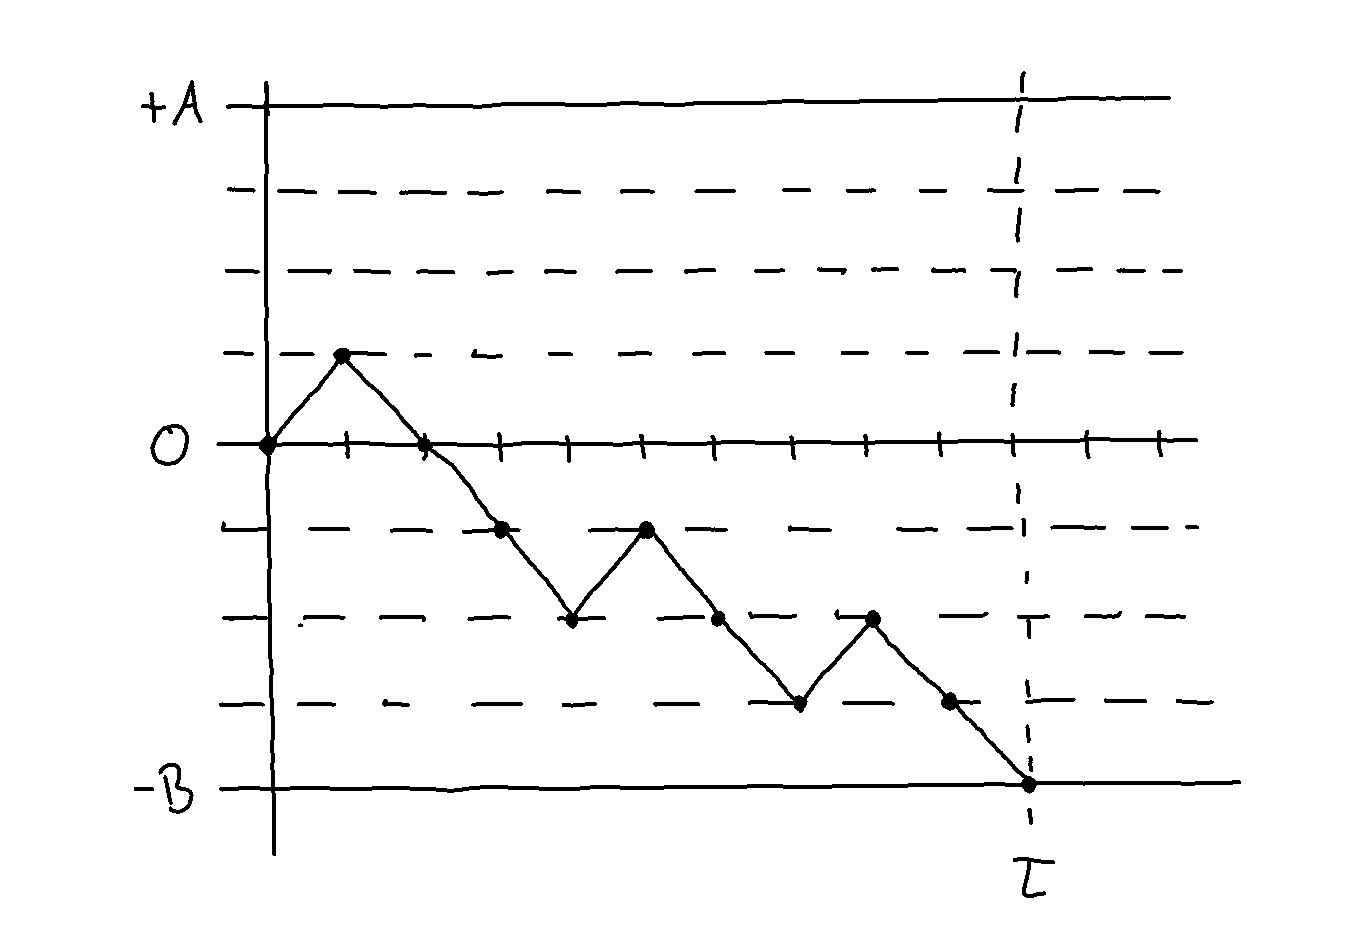
\includegraphics[width=0.75\textwidth]{pics/Sketch0.png}
			\caption{Beispiel für finite-Elemente-Funktionen in 1D}
			\label{AbbFiniteFunktionen}
		\end{center}
	\end{figure}
\end{definition}

\begin{bemerkung}\
	\begin{itemize}
		\item Für $m=k-1$ erhält man Splines.
		\item $\begin{aligned}
			S_h^{k,m}\subseteq H^{m+1}(\Omega)
		\end{aligned}$ wegen Satz \ref{satz1.4}
		\item $\begin{aligned}
			S_h^{0,m}
		\end{aligned}$ sind konstante Funktionen auf $(0,1)$ für $m\geq0$
		\item Die Räume haben folgende Dimensionen:
		\begin{align*}
			\dim\left(S_h^{k,-1}\right)&=(n+1)\cdot(k+1)\\
			\dim\left(S_h^{k,m}\right)&=\dim\left(S_h^{k,-1}\right)-n\cdot(m+1)\\
			\dim\left(S_{h,0}^{k,m}\right)&=\dim\left(S_h^{k,m}\right)-2
		\end{align*}
		Konkrete wichtige Beispiele:
		\begin{align*}
			\dim\left(S_h^{k,0}\right)&=(n+1)\cdot(k+1)-n\\
			\dim\left(S_{h,0}^{k,0}\right)&=(n+1)\cdot(k+1)-n-2=(n+1)\cdot(k-1)+n\\
			\dim\left(S_{h,0}^{1,0}\right)&=(n+1)\cdot 2-n-2=n\\
			\dim\left(S_{h,0}^{2,0}\right)&=(n+1)\cdot 3-n-2=2\cdot n+1
		\end{align*}
	\end{itemize}
\end{bemerkung}

Sei $\lbrace\varphi_j\rbrace_{j\in J}$ eine Basis von $S_h^{k,0}$
und Lösung $u_h\in S_{h,0}^{k,0}: u_h=\sum\limits_j u_j\cdot\varphi_j$\\
Diskretes Problem: Finde $u_h\in S_{h,0}^{k,0}$ so, dass
\begin{align*}
	&a(u_h,\varphi_h)=l(\varphi_h)&\qquad&\forall \varphi_h\in S_{h,0}^{k,0}\\
	\Longleftrightarrow &a(u_h,\varphi_i)=l(\varphi_i)&\qquad&\forall i
\end{align*}
In Matrix-Notation ergibt dies Folgendes:
\begin{align*}
	&A=(a_{i,j}),&&a_{i,j}:=a(\varphi_j,\varphi_i)\\
	&b=(b_i),&&b_i:=l(\varphi_i\nl
	&\qquad\Longleftrightarrow A\cdot U=b,\qquad U=(u_i)
\end{align*}
Hierbei heißt $A$ \textbf{Stiffness-Matrix}.

\begin{align*}
	S^{1,0}_{h,0}&=\text{span}\big\lbrace\varphi_i:1\leq i\leq n\big\rbrace,\qquad
	\varphi_i(t)=\left\lbrace\begin{array}{cl}
		\frac{t-t_{i-1}}{h_{i-1}}, &\falls t\in I_{i-1}\\
		\frac{t_{i+1}-t}{h_i}, &\falls t\in I_i\\
		0, &\sonst
	\end{array}\right.\\
	\big(\text{supp}(\varphi_i) &= [t_{i-1}, t_{i+1}]\big)\\
	\implies a_{i,j}&=0\text{ für }|i-j|>1\implies A\text{ ist Tridiagonalmatrix}
\end{align*}

\begin{figure}[!ht]
	\begin{center}
		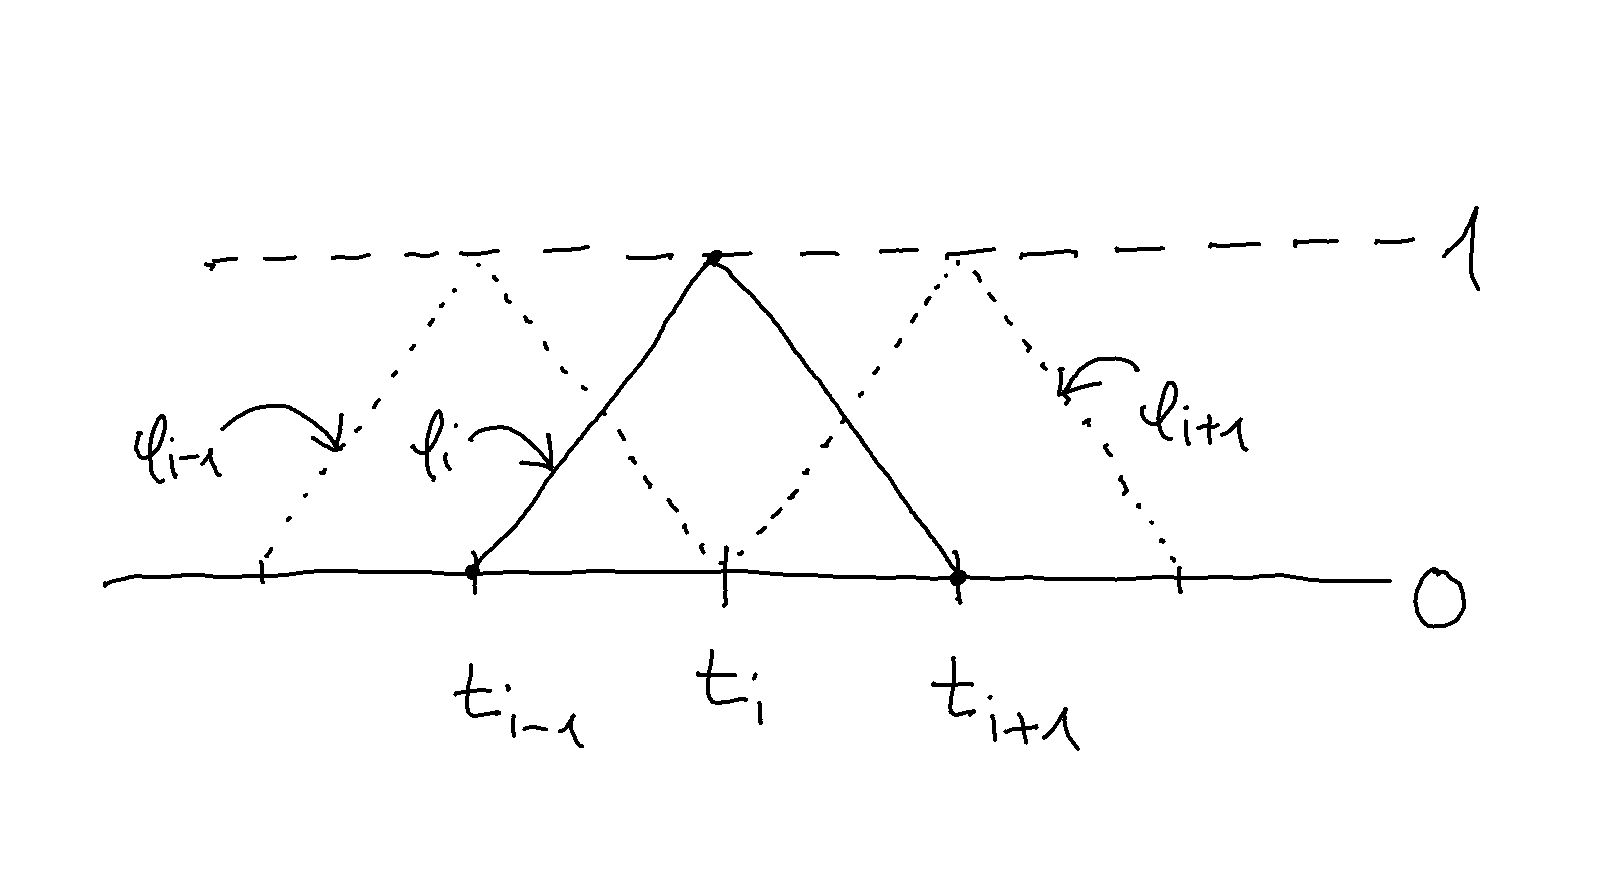
\includegraphics[width=0.75\textwidth]{pics/Sketch1.png}
		\caption{Hut-Funktionen}
		\label{AbbHutFunktionen}
	\end{center}
\end{figure}

\begin{figure}[!ht]
	\begin{center}
		\centering
\begin{tikzpicture}[scale=1]

% Achsen
\draw (0,0) -- ++(0,1.2);
\draw (0,0) -- ++(4,0);

% Funktion
\draw[red] (0,0) -- ++(2.5,0) -- ++(0.5,1) -- ++(0.5,-1) -- ++(0.5,0);
	
% Anstrich Y-Achse 
\draw (-0.1,1) -- ++(0.2,0);
	
% Anstriche X-Achse
\draw (0.5,-0.1) -- ++(0,0.2);
\draw (1  ,-0.1) -- ++(0,0.2);
\draw (1.5,-0.1) -- ++(0,0.2);
\draw (2  ,-0.1) -- ++(0,0.2);
\draw (2.5,-0.1) -- ++(0,0.2);
\draw (3  ,-0.1) -- ++(0,0.2);
\draw (3.5,-0.1) -- ++(0,0.2);
	
	
\filldraw[red] (0.5,0) circle (1.5pt);
\filldraw[red] (1  ,0) circle (1.5pt);
\filldraw[red] (1.5,0) circle (1.5pt);
\filldraw[red] (2  ,0) circle (1.5pt);
\filldraw[red] (2.5,0) circle (1.5pt);
\filldraw[red] (3  ,1) circle (1.5pt);
\filldraw[red] (3.5,0) circle (1.5pt);
	
	
\node at (-0.3,1) {1};
\node at (3.5,1) {$\varphi_j$};
\end{tikzpicture}

		\caption{einzelne Hut-Funktion}
		\label{AbbPhiHat}
	\end{center}
\end{figure}

\begin{align*}
	S_{h,0}^{2,0}&=\spann\big\lbrace\varphi_1,\ldots,\varphi_n,\psi_0,\ldots,\psi_n\big\rbrace,\qquad
	\psi_i(t)=\left\lbrace\begin{array}{cl}
		4\cdot\frac{(t-t_i)\cdot(t_{i+1}-t)}{h_i^2}, &\falls t\in I_i\\
		0 &\sonst
	\end{array}\right.
\end{align*}

\begin{figure}[!ht]
	\begin{center}
		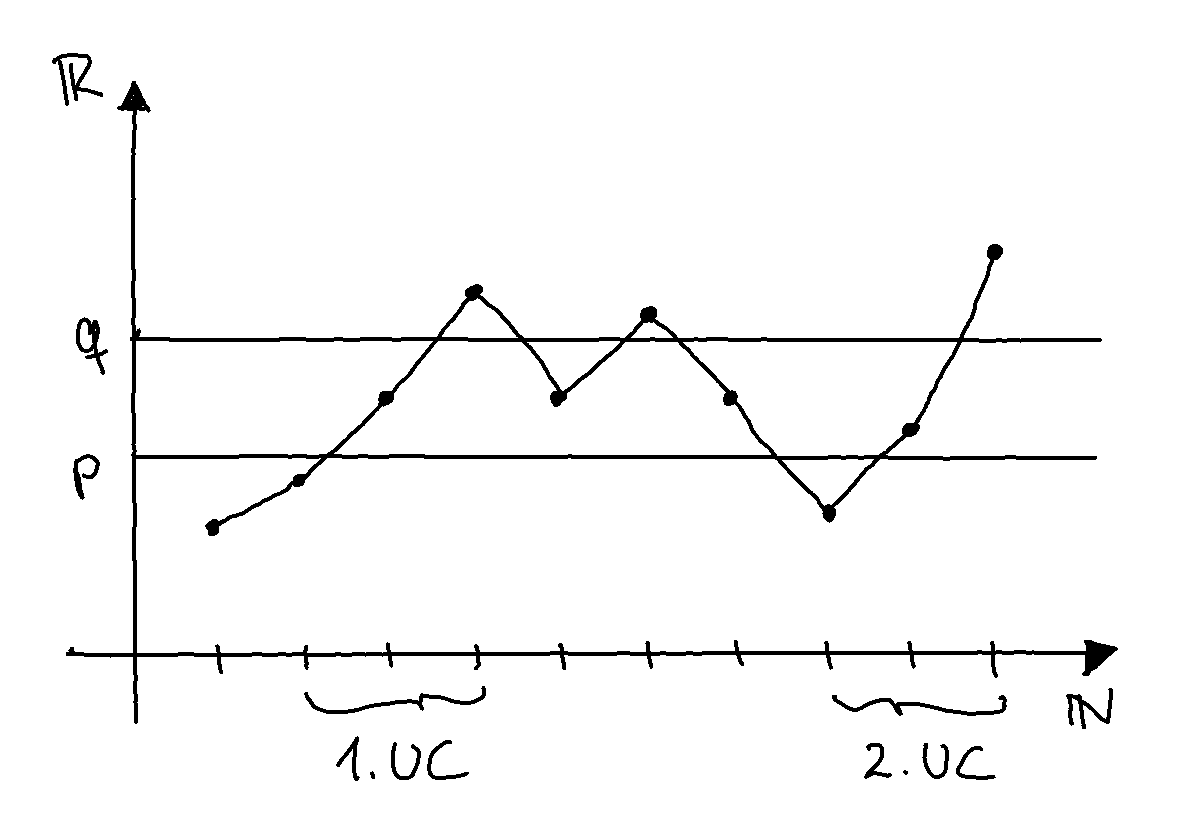
\includegraphics[width=0.5\textwidth]{./pics/Sketch2.png}
		\caption{einzelne zweifach diffbare finite-Elemente-Funktion}
		\label{AbbFiniteElementeFunktionZweifachDiffbar}
	\end{center}
\end{figure}

Die Stiffness-Matrix $A$ lässt sich als Blockmatrix schreiben:
\begin{align*}
	A=\begin{pmatrix}
		A_{LL} & A_{LQ}\\
		A_{QL} & A_{QQ}
	\end{pmatrix}
\end{align*}
wobei $A_{QQ}$ eine Diagonalmatrix ist. Somit:
\begin{align*}
	\begin{pmatrix}
		A_{LL} & A_{LQ}\\
		A_{QL} & A_{QQ}
	\end{pmatrix}\cdot\begin{pmatrix}
		U_L\\ U_Q
	\end{pmatrix}=
	\begin{pmatrix}
		b_L\\ b_Q
	\end{pmatrix}
\end{align*}
Dieses System von Gleichungen ist äquivalent zu:
\begin{align*}
	\big(A_{LL}-A_{LQ}\cdot A^{-1}_{QQ}\cdot A_{QL}\big)\cdot U_L&= b_L-A_{LQ}\cdot A^{-1}_{QQ}\cdot b_Q\\
	A_{QQ}\cdot U_Q&= b_Q-A_{QL}\cdot U_L
\end{align*}

\begin{theorem}[Approximationseigenschaft von 1D finiten Elementen]\label{theorem4.2}\enter
	Sei $u\in H^{k+1}(\Omega)\cap H^{1}_0(\Omega)$ für ein $k\geq1$. Dann gilt:
	\begin{align*}
		\inf\limits_{v_h\in S_{h,0}^{k,0}}\big|u-v_h\big|_{1,2}\leq h^k\cdot|u|_{k+1,2}
	\end{align*}
	(Hierbei ist $h$ wie oben der Maximalabstand.)
\end{theorem}

\begin{proof}
	Definiere Intervallweise die Funktion auf $I_i$ durch
	\begin{align*}
		v_h^\ast(t):=L_i(t)\qquad\forall t\in I_i,~\forall i\in\lbrace1,\ldots,n\rbrace
	\end{align*}
	wobei die $L_i$ die Lagrange-Interpolationen in $P_k$ bzgl. $t_i+\frac{s}{h}\cdot h_i,~0\leq j\leq h$ sind.\\
	Offenbar gilt $v_h^\ast\in S^{k,0}_{h,0}$. \\
	$u-v_n^\ast$ in $\overline{I_i}=[t_i,t_{i+1}]$ hat $(k+1)$ Nullen wegen der Interpolation. Somit hat $\big(u-v_h^\ast)^{(\mu)}$ $(k+1-\mu)$ Nullen.
	\begin{align*}
		\big|u-v_h^\ast\big|_{\mu,2,I_i}
		&=\left\Vert \big(u-v_h^\ast\big)^{(\mu)}\right\Vert_{0,2,I_i}\\
		&\stackrel{}{\leq}
		h_i\cdot\left|\big(u-v_h^\ast\big)^{(\mu)}\right|_{1,2,I_i}\\
		&=h_i\cdot\left|\big(u-v_h^\ast\big)^{(\mu+1)}\right|_{0,2,I_i}\\
		&\leq h_i\cdot\left|u-v_h^\ast\right|_{\mu+1,2,I_i}\\
		\implies
		\big|u-v_h^\ast\big|_{1,2,I_i}
		&\leq h_i^k\cdot\big|u-v_h^\ast\big|_{k+1,2,I_i} \\
		\overset{v_h^\ast|_{I_i}\in P_k}&=
		h_i^k\cdot |u|_{k+1,2,I_i}
	\end{align*}
	Somit folgt
	\begin{align*}
		\big| u-v_h^\ast\big|_{1,2,\Omega}
		&=\left(\sum\limits_{i=1}^n\big|u-v_h^\ast\big|^2_{1,2,I_i}\right)^{\frac{1}{2}}\\
		&\leq\left(\sum\limits_{i=1}^n \underbrace{h_i^{2\cdot k}}_{\leq h^{2\cdot k}} \big|u\big|^2_{k+1,2,I_i}\right)^{\frac{1}{2}}\\
		&\leq h^k\cdot |u|_{k+1,2,\Omega}
	\end{align*}
\end{proof}

\begin{lemma}\label{lemma4.3}
	Sei $u\in H^1((a,b))$ mit der Eigenschaft
	\begin{align*}
		\exists t^\ast\in[a,b]:u(t^\ast)=0.
	\end{align*}
	Dann gilt:
	\begin{align*}
		\Vert  u\Vert_{L^\infty}:=\max\limits_{t\in [a,b]}\big|u(t)\big|&\leq(b-a)^{\frac{1}{2}}\cdot |u|_{1,2}\\
		\Vert u\Vert_{0,2}&\leq(b-a)\cdot|u|_{1,2}
	\end{align*}
	Für alle $u\in H^1_0((a,b))$ gilt:
	\begin{align*}
		\left(1+(b-a)^2\right)^{\frac{1}{2}}\cdot\Vert u\Vert_{1,2}\leq|u|_{1,2}\leq\Vert u\Vert_{1,2}
	\end{align*}
\end{lemma}

\subsection*{Sturm-Liouville Problem}
\begin{align}\label{eqSturmLiouvillePDE}\tag{SturmLiouville}
	\left\lbrace\begin{array}{rll}
		-\big(p(x)\cdot u'(x)\big)'+q(x)\cdot u(x) &= f(x) &\text{ in } (0,1)\\
		u(0)=u(1)&=0 &
	\end{array}
	\right.
\end{align}
wobei
\begin{align*}
	&f\in L^2((0,1)),\\
	&q\in C\big([0,1]\big), &&q(x)\geq0\quad\forall x\in[0,1], \\
	&p\in C\big([0,1]\big), &&p(x)\geq p_0>0\quad\forall x\in [0,1]
\end{align*}
\begin{align*}
	a(v,w)=\int\limits_0^1 p(x)\cdot v'(x)\cdot w'(x)+q(x)\cdot v(x)\cdot w(x)\d x
\end{align*}

\begin{theorem}\label{theorem4.4}
	Sei $u\in H^1_0\big((0,1)\big)$ die eindeutige schwache Lösung von \eqref{eqSturmLiouvillePDE} und $u_h$ die zugehörige Lösung in $S_{h,0}^{k,0}$.
	Falls $u\in H^{k+1}\big((0,1)\big)$, dann gilt:
	\begin{align*}
		|u-u_h|_{1,2}&\leq c_1\cdot h^k\cdot |u|_{k+1,2}\\
		\Vert u-u_h\Vert_{0,2}&\leq c_1\cdot h^k\cdot |u|_{k+1,2}\\
		\mit c_1&=\frac{2}{p_0}\cdot\max\limits\big\lbrace \Vert p\Vert_{C^0},\Vert q\Vert_{C^0}\big\rbrace
	\end{align*}
	Falls zusätzlich die schwache Formulierung für alle $\varphi\in L^2\big((0,1)\big)$ eine eindeutige schwache Lösung
	\begin{align*}
		u_\varphi\in H^2\big((0,1)\big)\cap H^1_0\big((0,1)\big)\mit |u_\varphi|_{2,2}\leq c_2\cdot\Vert \varphi\Vert_{0,2}
	\end{align*}
	liefert, dann gilt
	\begin{align*}
		\big\Vert u-u_h\big\Vert_{0,2}\leq c_3\cdot h^{k+1}\cdot |u|_{k+1,2}
		\mit c_3=\frac{4\cdot c_2}{p_0}\cdot\max\limits\left\lbrace\Vert p\Vert^2_{C^0},\Vert q\Vert^2_{C^0}\right\rbrace
	\end{align*}
\end{theorem}

\subsection{FEM in 2D}

Nun der zweidimensionale Fall: Sei $\Omega\subseteq\R^2$ ein beschränktes Polygon. 
Nun zerlegen wir das Polygon in Dreiecke. 
Dieses Verfahren heißt \textbf{Dekomposition / Triangulation.} 
Dadurch erhalten wir eine Menge von \underline{offenen} (nach Konvention) Dreiecken $\lbrace K_i\rbrace_{i\in\lbrace1,\ldots,N\rbrace}$ mit den Eigenschaften:

\begin{enumerate}[label=(\roman*)]
	\item $\begin{aligned}
		\overline{\Omega}=\bigcup\limits_{i=1}^N \overline{K_i}
		\end{aligned}$
	\item $\begin{aligned}
		i\neq j\implies K_i\cap K_j=\emptyset
	\end{aligned}$
	\item Zulässigkeit: $\overline{K_i}\cap\overline{K_j}$ für $i\neq j$ ist
	\begin{itemize}
		\item leer oder
		\item ein einziger Punkt oder
		\item eine \ul{gemeinsame} Kante.
	\end{itemize}

	\begin{figure}[!ht]
		\begin{center}
			\begin{tikzpicture}[scale=1]

     
	
    % fill triangles
    \fill[red!40!white]   (0,0) -- ++(1,-0.5) -- ++(0.25,0.5) --cycle;
    \fill[blue!40!white]  (0,0) -- ++(1.25,0) --++(-0.75,0.25) --cycle;
    \fill[green!20!white]   (1.25,0) --++(-0.75,0.25) --++(1.75,0.25) --cycle;
    \fill[yellow!20!white]   (0.5,0.25) --++(1.75,0.25) --  ++(-2.75,0.5) --cycle;
	 
	% outline
	\draw (0,0) -- ++(1,-0.5) -- ++(0.25,0.5)-- ++(1,0.5) -- ++(-2.75,0.5)-- ++(1,-0.75)--cycle;

	% this is unrobust
	\draw (0,0) -- ++(1.25,0) --++(-0.75,0.25) --++(1.75,0.25);

\end{tikzpicture}
			\caption{beispielhafte Triangulation, $K_i$ disjunkt}
			\label{AbbTriangulierung}
		\end{center}
	\end{figure}

	\begin{figure}[!ht]
		\begin{center}
			\begin{tikzpicture}[scale=1]

	% outline
	\draw (0,0) -- ++(1.5,-1) -- ++(1.5,1)-- ++(-1.5,1) -- cycle;
	\draw (1.5,-1) -- ++(0,2);
	\draw (1.5,0) -- ++(1.5,0);
	
	% red cross
	\draw[thick,red] (0,-1) --++ (3,2);

	% dot middle
	\filldraw (1.5,0) circle (1.6pt);

\end{tikzpicture}
			\caption{Unzulässige Triangulation}
			\label{AbbUnzulaessigeTriangulierung}
		\end{center}
	\end{figure}
\end{enumerate}

Die Triangulation $\T$ ist formal definiert als Menge der Teildreiecke, also
\begin{align*}
	\T:=\lbrace K_1,\ldots,K_N\rbrace.
\end{align*} 

\subsection*{Raum der stetigen stückweise linearen Funktionen}
\begin{align*}
	V_h&:=\left\lbrace
	\begin{array}{rl}
		v\in C(\overline{\Omega}) : &v|_{K_i}\in P_1(K_i)~\forall i=1,\ldots,N,\\
		&v|_{\partial\Omega}=0
	\end{array}\right\rbrace
	\subseteq H^1_0(\Omega)\\
	P_1(K_i)&=\spann(\lbrace1,x,y\rbrace)\text{ (zwei-Dimensional, deshalb }x,y)\\
	P_2(K_i)&=\spann\big(\big\lbrace x^\alpha, |\alpha|\leq k\big\rbrace\big)\mit K\subseteq\R^d,~ x^{\alpha}:=x_1^{\alpha_1},\ldots,x_d^{\alpha_d}\\
	Q_k(K_i)&=\spann\big(\big\lbrace x^\alpha,\max\limits_i |\alpha_i|\leq k\big\rbrace\big)\\
	Q_1(K_i)&=\spann(\lbrace 1,x,y,xy\rbrace)\\
	\dim(V_h)&=\text{ Anzahl der inneren Knoten von der zulässigen Triangulierung}\\
\end{align*}

\begin{definition}[Finites Element]\enter %4.5
	Ein \textbf{finites Element} ist ein Tripel $(K,V,\Sigma)$ mit:
	\begin{enumerate}[label=(\roman*)]
		\item $K\subseteq\R^d$ ist nichtleer, offen, beschränkt und Lipschitz-berandet.
		\item $V=\big\lbrace f:K\to\R\big\rbrace$ ist endlich-dimensionaler Funktionenraum mit $m:=\dim(V)<\infty$. Sei $B_V:=\lbrace\varphi_1,\ldots,\varphi_m\rbrace$ eine Basis von $V$.
		Die Funktionen $v_i\in V$ heißen \textbf{lokale Basis / Shape-Funktionen / Form-Funktionen} genannt.
		\item Sei $\Sigma:=\lbrace N_1,\ldots,N_m\rbrace$ die eindeutige duale Basis zu $B_V$, d.h. es gilt (aus LAAG bekannt):
		\begin{align*}
			\forall i\in\lbrace 1,\ldots,m\rbrace:\exists! N_i\colon V\to\R:\forall j\in\lbrace1,\ldots,m\rbrace: N_i(\varphi_j)=\delta_{i,j}
		\end{align*}				
		Somit ist $\Sigma$ eine Basis von $V^\ast$ bestehend aus $m$ linearen Funktionalen $N_i$, den sogenannten \textbf{Nodal-Funktionalen / Freiheitsgrade / DOFs.}
	\end{enumerate}
\end{definition}

\begin{bemerkung} % war in VL anders
	Die Nodal-Funktional-Menge $\Sigma$ gilt: 
		\begin{align*}
			\Sigma\text{ ist Basis von }V^\ast\Longleftrightarrow\Sigma\text{ ist \textbf{$V$-unisolvent}, d. h.:}\\
			\forall (\alpha_1,\ldots,\alpha_m)\in\R^m:\exists! v\in V:\forall i\in\lbrace1,\ldots,m\rbrace:N_i(v)=\alpha_i
		\end{align*}
\end{bemerkung}

\begin{proof}
	\underline{Zeige Basis $\implies V$-unisolvenz:}\\
	Sei $i\in\lbrace1,\ldots,m\rbrace$ und $\alpha_i\in\R$ beliebig.\nl
	\underline{Existenz}:
	Da $B_V$ eine Basis von $V$ ist, gilt 
	\begin{align*}
		\forall v\in V:\exists v_1,\ldots,v_m\in\R:v=\sum\limits_{j=1}^m\varphi_j\cdot v_j
	\end{align*}
	und somit
	\begin{align*}
		N_i(v)
		=N_i\left(\sum\limits_{j=1}^m\varphi_j\cdot v_j\right)
		\overset{\text{Lin}}=
		\sum\limits_{j=1}^m v_j\cdot \underbrace{N_i(\varphi_j)}_{=\delta_{i,j}}=v_i\qquad\forall v\in V.
	\end{align*}
	Wähle als $v_i:=\alpha_i\in\R$.\nl
	\underline{Eindeutigkeit:}
	Seien $v,\tilde{v}\in V$ mit $N_i(v)=\alpha_i=N_i(\tilde{v})$.
	Dann gilt schon $v=\tilde{v}$, denn:
	\begin{align*}
		v_i=N_i(v)=\alpha_i=N_i(\tilde{v})=\tilde{v_i}\qquad\forall i\in\lbrace1,\ldots,m\rbrace	
	\end{align*}	
	\underline{Zeige $V$-unisolvenz $\implies$ Basis}:
	Nachrechnen. 
\end{proof}

Es ist sinnvoll und naheliegend für ein Finites-Element $(K,V,\Sigma)$ $\dim(V)=|\Sigma|=n$ zu wählen, mit $n$ Anzahl der Ecken des Polygons $K\subseteq\R^2$.
Nodal-Funktionale bilden Funktionen auf deren Werte an den "Ecken" ab.

\begin{definition}[affin äquivalente finite Elemente]\enter %4.6
	Zwei finite Elemente $(K,V,\Sigma)$ und $(\hat{K},\hat{V},\hat{\Sigma})$ heißen \textbf{affin äquivalent}
	\begin{align*}
		:\Longleftrightarrow\exists F:\R^d\to\R^d\text{ affin \& invertierbar v.d.F. }
		\hat{x}\mapsto B_k\cdot\hat{x}+b_k\mit B_k\in\R^{d\times d},b_k\in\R^d
	\end{align*}
	mit den Eigenschaften
	\begin{enumerate}[label=(\arabic*)]
		\item $\begin{aligned}
			K=F(\hat{K})
		\end{aligned}$
		\item $\begin{aligned}
			V=\Big\lbrace v: K\to\R~\Big|~\exists\hat{v}\in\hat{V}: v=\hat{v}\circ F^{-1}\Big\rbrace
		\end{aligned}$
		\item $\begin{aligned}
			\Sigma=\Big\lbrace N:V\to\R~\Big|~\exists\hat{N}\in\hat{\Sigma}: N(v)=\hat{N}(v\circ F)\Big\rbrace
		\end{aligned}$
	\end{enumerate}
\end{definition}

\begin{beisp}\
	\begin{figure}[H]
		\begin{center}
			\centering
\begin{tikzpicture}[scale=2]


\draw[thick] (0,0) -- ++(0,1) -- ++(1,-1)--cycle;
\filldraw (0,0)         circle (0.8pt);
\filldraw (0,0) ++(1,0) circle (0.8pt);
\filldraw (0,0) ++(0,1) circle (0.8pt);
\fill[black,font=\footnotesize] (0,0) node[below] {1 $(0,0)$}
								(0,0) ++(1,0) node[below] {2 $(1,0)$}
								(0,0) ++(0,1) node[above] {3 $(0,1)$};
								
\draw[thick] (2.2,0) -- ++(2,0) -- ++(-1,1)--cycle;
\filldraw (2.2,0)         circle (0.8pt);
\filldraw (2.2,0) ++(2,0) circle (0.8pt);
\filldraw (2.2,0) ++(1,1) circle (0.8pt);
\fill[black,font=\footnotesize] (2.2,0) node[below] {1 $(a_1,a_2)$}
								(2.2,0) ++(2,0) node[below] {2 $(b_1,b_2)$}
								(2.2,0) ++(1,1) node[above] {3 $(c_1,c_2)$};								
								
												
\node at (1.5,1) {$F$};				
\draw[thick,-to] (1.2,0.5) .. controls (1.4,0.8) and (1.9,0.9) .. (2.2, 0.8);
\draw[thick] (0,0) -- ++(0,1) -- ++(1,-1)--cycle;

\end{tikzpicture}

			\caption{affin äquivalente Triangulation}
			\label{AbbAffinEquivTriang}
		\end{center}
	\end{figure}

	\begin{align*}
		F:\left\lbrace\begin{array}{l}
			(0,0)\mapsto(a_1,a_2)\\
			(1,0)\mapsto(b_1,b_2)\\
			(0,1)\mapsto(c_1,c_2)
		\end{array}\right.
		\qquad\qquad
		\begin{matrix}
			\hat{N}_1(\hat{v})&=\hat{v}(0,0) &&N_1(v)=v(a_1,a_2)\\
			\hat{N}_2(\hat{v})&=\hat{v}(1,0) &&N_2(v)=v(b_1,b_2)\\
			\hat{N}_3(\hat{v})&=\hat{v}(0,1) &&N_3(v)=v(c_1,c_2)
		\end{matrix}
	\end{align*}
\end{beisp}

Sei $V$ ein Vektorraum mit Basis $\lbrace\varphi_1,\ldots,\varphi_m\rbrace$. Setze
\begin{align*}
	\Sigma&=\lbrace N_1,\ldots,N_m\rbrace\\
	M&=(m_{i,j}),\qquad m_{i,j}:=N_i(\varphi_j)\\
	M&\text{ invertierbar }\Longleftrightarrow \text{ unisolvent}
\end{align*}
Unisolvenz: Gegeben $\alpha_1,\ldots,\alpha_m\in\R$. Gibt es ein eindeutiges $v\in V$
\begin{align*}
	N_i(v)&=\alpha_i,\qquad i\in\lbrace1,\ldots,m\rbrace\\
	\stackrel{v=\sum\limits_{j=1}^m c_j\cdot\varphi_j}{\Longleftrightarrow}\quad
	\sum\limits_{j=1}^m N_i(\varphi_j)\cdot c_j&=\alpha_i\\
	\Longleftrightarrow
	M\cdot c&=\alpha
\end{align*}

\begin{beispiel} % war nicht in VL
	Dreiecke:
	\begin{itemize}
		\item $P_0$: stückweise konstante FEM,\\ $\dim(P_0(K))=1$
		\item $P_1$: konformes stückweises linearen FEM, $\dim(P_1(K))=d+1\overset{d=2}{=}3$
		\item $P_2$: konforme stückweise quadratische FEM, $\dim(P_2(K))=\frac{(d+1)\cdot(d+2)}{2}=\overset{d=2}{=}6$
		\item $P_3$: konforme stückweise kubische FEM, $\dim(P_3(K))=\frac{(d+1)\cdot(d+2)\cdot(d+3)}{6}\overset{d=2}{=}10$
	\end{itemize}
	
	\begin{figure}[H] % oder ht!
		\begin{center}
			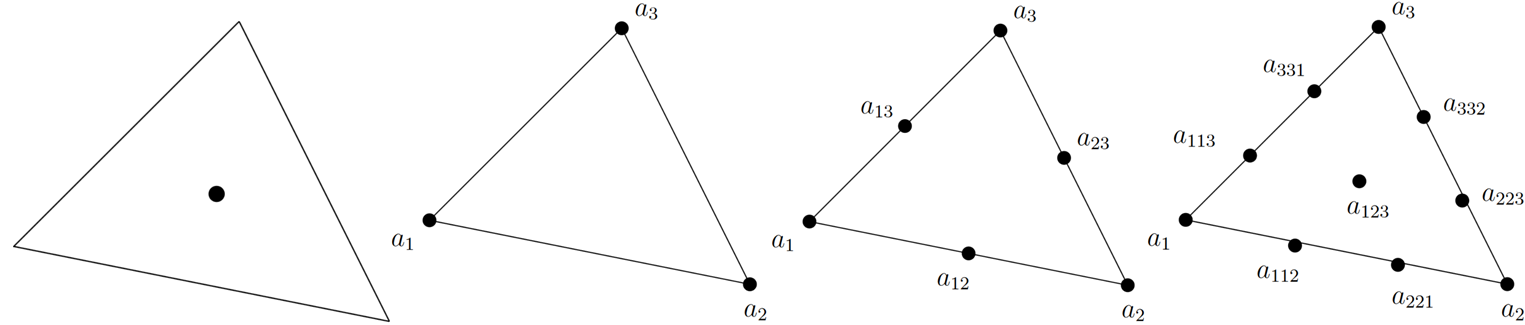
\includegraphics[width=1\textwidth]{./pics/FEM_Dreieck.png}
			\caption{Nodal Functionals für $P_0,P_1,P_2,P_3$}
			\label{AbbFEM-Dreieck}
		\end{center}
	\end{figure}

	Quadrate:
	\begin{itemize}
		\item $Q_0$: stückweise konstantes FEM: $\dim(Q_0(K))=1$
		\item $Q_1$: konforme stückweise $d$-lineare FEM, $\dim(Q_1(K))=2^d\overset{d=2}{=}4$
		\item $Q_2$: konforme stückweise $d$-dimensionalen FEM, $\dim(Q_2(K))=3^d\overset{d=2}{=}8$
		\item $Q_3$: konforme stückweise $d$-kubische FEM, $\dim(Q_3(K))=4^d\overset{d=2}{=}16$.
	\end{itemize}
	
	\begin{figure}[H] % oder ht!
		\begin{center}
			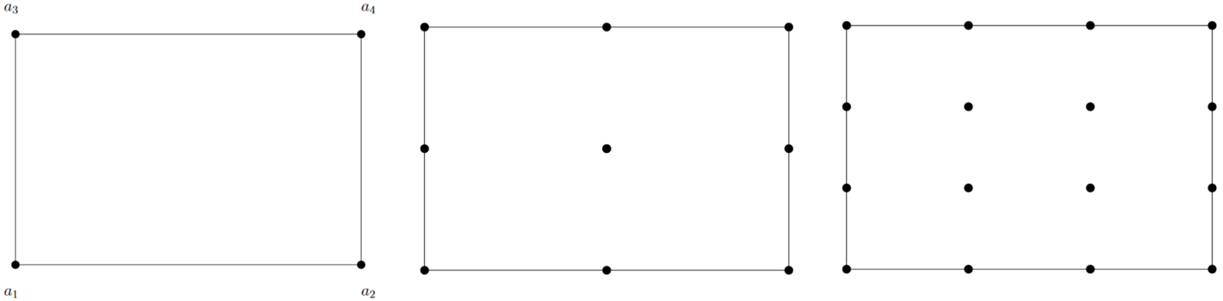
\includegraphics[width=1\textwidth]{./pics/FEM_Quadrat.png}
			\caption{Nodal Functionals für $Q_1,Q_2,Q_3$}
			\label{AbbFEM-Qudrat}
		\end{center}
	\end{figure}
\end{beispiel}

\begin{definition}[globales Nodal-Funktional / globale Freiheitsgrade (dof)]\enter
	Seien $(K,V,\Sigma)$ und $(K',V',\Sigma')$ Finite-Elemente.
	Zwei lokale Nodal-Funktionale $N_i^K\in\Sigma$ und $N_j^{K'}\in\Sigma'$ \textbf{gehören zum selben globalen Freiheitsgrad}, i.Z.
	\begin{align*}
		N_i^K\sim N_j^{K'}:\Longleftrightarrow N_i^K(\varphi|_K)=N_j^{K'}(\varphi|_{K'})\qquad\forall\varphi\in C^\infty(U)
	\end{align*}
	wobei $U\subseteq\Omega$ eine offene Menge mit der Eigenschaft $\overline{K\cup K'}\subseteq U$ ist.\\
	Anschaulich: Zwei Nodal-Funktionale sind $\sim$-äquivalent, wenn sie dieselbe Ecke beschreiben.
	$\sim$ ist eine Äquivalenzrelation.\\
	Die \textbf{Menge aller globalen Freiheitsgrade} einer Triangulation $\T=\lbrace K_1,\ldots,K_N\rbrace$ bezeichnen wir mit
	\begin{align*}
		\Sigma_h:=\left.\left(\bigcup\limits_{i=1}^N\bigcup\limits_{j=1}^m N_j^{K_i}\right)\right/\sim
	\end{align*}
	Für $[N]_\sim\in\Sigma_h$ bezeichne
	\begin{align*}
		\Lambda\big([N]_\sim\big):=\left\lbrace N\in[N]_\sim\right\rbrace
	\end{align*}		
	die Menge alle lokalen Freiheitsgrade $N$, die zu $[N]_\sim$ gehören.
\end{definition}

\begin{figure}[H] % oder ht!
	\begin{center}
		% This work is licensed under the Creative Commons
% Attribution-NonCommercial-ShareAlike 4.0 International License. To view a copy
% of this license, visit http://creativecommons.org/licenses/by-nc-sa/4.0/ or
% send a letter to Creative Commons, PO Box 1866, Mountain View, CA 94042, USA.
% vim: set noexpandtab:

% the following tikz picture was auto-generated by:
% https://www.mathcha.io/editor

\tikzset{every picture/.style={line width=0.75pt}} %set default line width to 0.75pt        

\begin{tikzpicture}[x=0.75pt,y=0.75pt,yscale=-1,xscale=1]
%uncomment if require: \path (0,300); %set diagram left start at 0, and has height of 300

%Shape: Rectangle [id:dp14549454055533384] 
\draw   (64,2.93) -- (345,2.93) -- (345,290.93) -- (64,290.93) -- cycle ;
%Straight Lines [id:da9627683453327494] 
\draw    (64,2.93) -- (345,290.93) ;


%Straight Lines [id:da9434997856090799] 
\draw    (345,2.93) -- (64,290.93) ;


%Straight Lines [id:da169571524037062] 
\draw    (100,130) ;


%Shape: Circle [id:dp7836721006446373] 
\draw   (186.18,146.69) .. controls (186.9,144.02) and (189.65,142.45) .. (192.31,143.18) .. controls (194.98,143.9) and (196.55,146.65) .. (195.82,149.31) .. controls (195.1,151.98) and (192.35,153.55) .. (189.69,152.82) .. controls (187.02,152.1) and (185.45,149.35) .. (186.18,146.69) -- cycle ;
%Shape: Circle [id:dp7887685534943322] 
\draw   (214.18,146.69) .. controls (214.9,144.02) and (217.65,142.45) .. (220.31,143.18) .. controls (222.98,143.9) and (224.55,146.65) .. (223.82,149.31) .. controls (223.1,151.98) and (220.35,153.55) .. (217.69,152.82) .. controls (215.02,152.1) and (213.45,149.35) .. (214.18,146.69) -- cycle ;
%Shape: Circle [id:dp792561043036806] 
\draw   (198.18,161.69) .. controls (198.9,159.02) and (201.65,157.45) .. (204.31,158.18) .. controls (206.98,158.9) and (208.55,161.65) .. (207.82,164.31) .. controls (207.1,166.98) and (204.35,168.55) .. (201.69,167.82) .. controls (199.02,167.1) and (197.45,164.35) .. (198.18,161.69) -- cycle ;
%Shape: Circle [id:dp5381851880499974] 
\draw   (200.18,131.69) .. controls (200.9,129.02) and (203.65,127.45) .. (206.31,128.18) .. controls (208.98,128.9) and (210.55,131.65) .. (209.82,134.31) .. controls (209.1,136.98) and (206.35,138.55) .. (203.69,137.82) .. controls (201.02,137.1) and (199.45,134.35) .. (200.18,131.69) -- cycle ;
%Shape: Circle [id:dp44002878595191575] 
\draw   (78.18,282.69) .. controls (78.9,280.02) and (81.65,278.45) .. (84.31,279.18) .. controls (86.98,279.9) and (88.55,282.65) .. (87.82,285.31) .. controls (87.1,287.98) and (84.35,289.55) .. (81.69,288.82) .. controls (79.02,288.1) and (77.45,285.35) .. (78.18,282.69) -- cycle ;
%Shape: Circle [id:dp42740284154555863] 
\draw   (67.18,267.69) .. controls (67.9,265.02) and (70.65,263.45) .. (73.31,264.18) .. controls (75.98,264.9) and (77.55,267.65) .. (76.82,270.31) .. controls (76.1,272.98) and (73.35,274.55) .. (70.69,273.82) .. controls (68.02,273.1) and (66.45,270.35) .. (67.18,267.69) -- cycle ;
%Shape: Circle [id:dp6205100758907591] 
\draw   (319.18,279.69) .. controls (319.9,277.02) and (322.65,275.45) .. (325.31,276.18) .. controls (327.98,276.9) and (329.55,279.65) .. (328.82,282.31) .. controls (328.1,284.98) and (325.35,286.55) .. (322.69,285.82) .. controls (320.02,285.1) and (318.45,282.35) .. (319.18,279.69) -- cycle ;
%Shape: Circle [id:dp12003747556472932] 
\draw   (331.18,265.69) .. controls (331.9,263.02) and (334.65,261.45) .. (337.31,262.18) .. controls (339.98,262.9) and (341.55,265.65) .. (340.82,268.31) .. controls (340.1,270.98) and (337.35,272.55) .. (334.69,271.82) .. controls (332.02,271.1) and (330.45,268.35) .. (331.18,265.69) -- cycle ;
%Shape: Circle [id:dp3476040811313178] 
\draw   (333.18,19.69) .. controls (333.9,17.02) and (336.65,15.45) .. (339.31,16.18) .. controls (341.98,16.9) and (343.55,19.65) .. (342.82,22.31) .. controls (342.1,24.98) and (339.35,26.55) .. (336.69,25.82) .. controls (334.02,25.1) and (332.45,22.35) .. (333.18,19.69) -- cycle ;
%Shape: Circle [id:dp21135819336466033] 
\draw   (323.18,9.69) .. controls (323.9,7.02) and (326.65,5.45) .. (329.31,6.18) .. controls (331.98,6.9) and (333.55,9.65) .. (332.82,12.31) .. controls (332.1,14.98) and (329.35,16.55) .. (326.69,15.82) .. controls (324.02,15.1) and (322.45,12.35) .. (323.18,9.69) -- cycle ;
%Shape: Circle [id:dp08585658948454522] 
\draw   (78.18,9.69) .. controls (78.9,7.02) and (81.65,5.45) .. (84.31,6.18) .. controls (86.98,6.9) and (88.55,9.65) .. (87.82,12.31) .. controls (87.1,14.98) and (84.35,16.55) .. (81.69,15.82) .. controls (79.02,15.1) and (77.45,12.35) .. (78.18,9.69) -- cycle ;
%Shape: Circle [id:dp07079948382140533] 
\draw   (65.18,21.69) .. controls (65.9,19.02) and (68.65,17.45) .. (71.31,18.18) .. controls (73.98,18.9) and (75.55,21.65) .. (74.82,24.31) .. controls (74.1,26.98) and (71.35,28.55) .. (68.69,27.82) .. controls (66.02,27.1) and (64.45,24.35) .. (65.18,21.69) -- cycle ;
%Shape: Circle [id:dp6214173079072771] 
\draw  [color={rgb, 255:red, 208; green, 2; blue, 27 }  ,draw opacity=1 ] (179.5,146.93) .. controls (179.5,133.13) and (190.69,121.93) .. (204.5,121.93) .. controls (218.31,121.93) and (229.5,133.13) .. (229.5,146.93) .. controls (229.5,160.74) and (218.31,171.93) .. (204.5,171.93) .. controls (190.69,171.93) and (179.5,160.74) .. (179.5,146.93) -- cycle ;
%Shape: Circle [id:dp8527921748422009] 
\draw  [color={rgb, 255:red, 208; green, 2; blue, 27 }  ,draw opacity=1 ] (314.69,274.39) .. controls (314.69,265.8) and (321.66,258.82) .. (330.26,258.82) .. controls (338.85,258.82) and (345.82,265.8) .. (345.82,274.39) .. controls (345.82,282.99) and (338.85,289.96) .. (330.26,289.96) .. controls (321.66,289.96) and (314.69,282.99) .. (314.69,274.39) -- cycle ;
%Shape: Circle [id:dp9683122242620462] 
\draw  [color={rgb, 255:red, 208; green, 2; blue, 27 }  ,draw opacity=1 ] (316.12,15.82) .. controls (316.12,7.23) and (323.09,0.26) .. (331.69,0.26) .. controls (340.29,0.26) and (347.26,7.23) .. (347.26,15.82) .. controls (347.26,24.42) and (340.29,31.39) .. (331.69,31.39) .. controls (323.09,31.39) and (316.12,24.42) .. (316.12,15.82) -- cycle ;
%Shape: Circle [id:dp7791705596437565] 
\draw  [color={rgb, 255:red, 208; green, 2; blue, 27 }  ,draw opacity=1 ] (61.74,17.18) .. controls (61.74,8.58) and (68.71,1.61) .. (77.31,1.61) .. controls (85.91,1.61) and (92.88,8.58) .. (92.88,17.18) .. controls (92.88,25.77) and (85.91,32.74) .. (77.31,32.74) .. controls (68.71,32.74) and (61.74,25.77) .. (61.74,17.18) -- cycle ;
%Shape: Circle [id:dp5325582065155569] 
\draw  [color={rgb, 255:red, 208; green, 2; blue, 27 }  ,draw opacity=1 ] (62.12,275.26) .. controls (62.12,266.66) and (69.09,259.69) .. (77.69,259.69) .. controls (86.29,259.69) and (93.26,266.66) .. (93.26,275.26) .. controls (93.26,283.85) and (86.29,290.82) .. (77.69,290.82) .. controls (69.09,290.82) and (62.12,283.85) .. (62.12,275.26) -- cycle ;

% Text Node
\draw (111,139) node  [align=left] {K1};
% Text Node
\draw (201,233) node  [align=left] {K2};
% Text Node
\draw (207,59) node  [align=left] {K3};
% Text Node
\draw (288,142) node  [align=left] {K4};


\end{tikzpicture}














		\caption{Hier werden die 12 DOFs der 4 FEMs per Äquivalenzrelation (rot) zu 5 globalen DOFs zusammengefasst.}
		\label{AbbGlobalDegreesOfFreedom}
	\end{center}
\end{figure}

\begin{definition}[Raum der finiten Elemente]\enter
	Sei $\T_h=\lbrace K_1,\ldots,K_N\rbrace$ eine Triangulation von $\Omega$ und seien\\ $\big((K_i,V_i(K_i),\Sigma_i(K_i)\big),i\in\lbrace1,\ldots,N\rbrace$ die zugehörigen Finite-Elemente.\\
	Ein \textbf{Finite-Elemente-Raum} $V_h$ ist gegeben durch
	\begin{align*}
		V_h:=\Bigg\lbrace v=(v_{K})_{K\in\T_h}\colon\bigcup\limits_{i=1}^N K_i\to\R\Bigg|
		\begin{array}{c}
			\forall [N]_\sim\in\Sigma_h:\forall N_i^{K},N_j^{K'}\in\Lambda([N]_\sim):\\
			N_i^{K}(v|_K)=N_j^{K'}(v|_{K'})
		\end{array}
		\Bigg\rbrace
	\end{align*}
	wobei $(K,V(K),\Sigma(K)),K\in\T_h$ finite Elemente sind.
	Im FEM-Raum liegen praktisch alle Funktionen $v:\Omega\to\R$ und es gibt eine Art globales Nodal-Funktional $N:(\Omega\to\R)\to\R$ (globales DOF), siehe Abbildung \ref{AbbGlobalDegreesOfFreedom}.
	Eine Funktion $v_h\in V_h$ ist eindeutig bestimmt durch die Werte des globalen DOFs $N(v_h)$.
\end{definition}

Familie aller affin äquivalenten Finiten-Elementen
\begin{align*}
	\big(K,V(K),\Sigma(K)\big)\sim\big(\hat{K},\hat{V},\hat{\Sigma}\big)
\end{align*}
Interpolation:
\begin{align*}
	I_h(v):=\sum\limits_{i=1}^n N_i(v)\cdot\varphi_i\in V_h
\end{align*}
wobei $\Sigma_h=\lbrace N_1,\ldots,N_n\rbrace\text{ und }\lbrace\varphi_1,\ldots,\varphi_n\rbrace$ eine Basis von $V_h$ ist mit der Eigenschaft $N_i(\varphi_j)=\delta_{i,j}$.\nl
\textbf{Wichtig:} Die Interpolationsfunktion erfüllt eine Lokalisierungseigenschaft:
\begin{align*}
	\big(I_h(v)\big)\big|_K&=I_h^K\big(v|_K\big)\quad\text{wobei}\\ I_h^K(v)&=\sum\limits_{i=1}^{m_K} N_i^{(K)}(v)\cdot\varphi_i^K,\qquad N_i^K(\varphi_j^K)=\delta_{i,j}\qquad\Sigma(K)=\left\lbrace N_1^K,\ldots,N_{m_K}^K\right\rbrace
\end{align*}

\begin{theorem}\label{theorem4.9}
	Seien $K,\hat{K}\subseteq\R^d$ zwei affin äquivalente offene  Teilmengen des $\R^d$, d. h. es existiert eine affine bijektive Abbildung
	\begin{align*}
		F:\hat{K}\to K,\qquad \hat{x}\mapsto B_K\cdot\hat{x}+ b_K\qquad\mit B_K\in\R^{d\times d}\text{ invertierbar und }b_K\in\R^d
	\end{align*}
	Falls $v\in W^{m,p}(K)$ für $m\geq0,p\in[1,\infty)$, dann gehört $\hat{v}:=v\circ F$ zu $W^{m,p}(\hat{K})$ und wir erhalten
	\begin{align*}
		\big|\hat{v}\big|_{m,p,\hat{K}}\leq c\cdot\Vert B_K\Vert^m\cdot\big|\det(B_K)\big|^{-\frac{1}{p}}\cdot|v|_{m,p,K}
	\end{align*}
	wobei $c=c(m,d)$ eine Konstante ist und $\Vert\cdot\Vert$ eine Matrixnorm, die durch die euklidische Vektornorm induziert wird.\\
	Zusätzlich gilt:
	\begin{align*}
		|v|_{m,p,K}&\leq c\cdot\Vert B_K^{-1}\Vert^m\cdot\big|\det(B_K)\big|^{\frac{1}{p}}\cdot|\hat{v}|_{m,p,\hat{K}}\\
		F^{-1}(x)&=B_K^{-1}\cdot x-B_K^{-1}\cdot b_K
	\end{align*}
\end{theorem}

\begin{lemma}\label{lemma4.10}
	Seien $K,\hat{K}$ affin äquivalent mit $F(\hat{x})=B_K\cdot\hat{x}+b_K$. Dann gilt:
	\begin{align*}
		\Vert B_K\Vert&\leq\frac{h_K}{\hat{\rho}},\qquad\Vert B_K^{-1}\Vert\leq\frac{\hat{h}}{\rho_K}\qquad\text{wobei}\\
		h_K&:=\diam(K):=\sup\limits_{x,y\in K}\Vert x-y\Vert\\
		\rho_K&:=\sup\big\lbrace\diam(S):S\subseteq K\text{ Sphäre}\big\rbrace
	\end{align*}
\end{lemma}

\begin{proof}
	\begin{align*}
		\Vert B_K\Vert&=\sup\limits_{z\neq0}\frac{\Vert B_K \cdot z\Vert}{\Vert z\Vert}=\frac{1}{\hat{\rho}}\cdot\sup\limits_{\Vert z\Vert=\hat{\rho}}\Vert B_K \cdot z\Vert
	\end{align*}
	Für alle $\eta$ mit $\Vert \eta\Vert=\hat{\rho}$ existieren zwei Punkte $\hat{x},\hat{y}\in\hat{K}$ so, dass $\eta=\hat{x}-\hat{y}$. Seien $x=F(\hat{x}),y=F(\hat{y})$. Dann gilt:
	\begin{align*}
		x-y&=B_K\cdot\hat{x}+b_K-\big(B_K\cdot\hat{y}+b_K\big)=B_K\cdot(\hat{x}-\hat{y})=B_K \cdot \eta\\
		\Vert B_K\cdot \eta\Vert&=\Vert x-y\Vert\leq h_K\\
		\implies \Vert h_K\Vert&\leq\frac{1}{\hat{\rho}}\cdot\sup\limits_{\Vert y\Vert=\hat{\rho}}\underbrace{\Vert B_K\cdot \eta\Vert}_{\leq h_K}\leq\frac{h_K}{\hat{\rho}}
	\end{align*}
\end{proof}

\begin{lemma}[Deny-Lions]\label{lemma4.11DenyLions}\enter
	Sei $P_r(K)$ der Raum aller Polynome mit höchstens Grad $r$. Dann gilt:
	\begin{align*}
		\exists c(K)>0:\inf\limits_{P\in P_r(K)}\Vert v\pm P\Vert_{r+1,p,K}\leq c(K)\cdot |v|_{r+1,p,K}\qquad\forall v\in W^{r+1,p}(K)
	\end{align*}
	(Hier $\pm$, da es egal ist, ob $-$ oder $+$, da $P\in P_r(K)\gdw -P\in P_r(K)$.)
\end{lemma}

\begin{proof}
	\begin{align*}
		n:=\dim \big(P_r(K)\big)=\begin{pmatrix}
			r+d\\ d
		\end{pmatrix}\text{ (Binomialkoeffizient)}
	\end{align*}
	Setze  für $\alpha\in\N_0^d\mit|\alpha|\leq r $:
	\begin{align*}
		N_\alpha:W^{r+1,p}(K)\to\R,\qquad v\mapsto\int\limits_K D^\alpha v\d x\\
		\alpha\longleftrightarrow x^\alpha =\prod\limits_{i=1}^d x_i^{\alpha_i}
	\end{align*}
	Also ist $\big\lbrace N_\alpha:|\alpha|\leq r\big\rbrace$ unisolvent auf $P_r(K)$.
	\begin{align*}
		\implies\left.
		\begin{array}{cl}
			N_\alpha(p)=0, &\forall |\alpha|\leq r \\
			p\in P_r(K)&
		\end{array}
		\right\rbrace
		\implies p\equiv 0
	\end{align*}
	Wir werden die Ungleichung
	\begin{align}\label{eqProof4.11Stern}\tag{$\ast$}
		\Vert v\Vert_{r+1,p,K}\leq c(K)\cdot\left(|v|_{r+1,p,K}+\sum\limits_{|\alpha|\leq r}\big|N_\alpha (r)\big|\right)\qquad\forall v\in W^{r+1,p}(K)
	\end{align}
	indirekt zeigen. Angenommen, diese Ungleichung gilt nicht. Dann gibt es eine Folge $(v_l)_{l\in\N}$ mit
	\begin{align}
		\Vert v_l\Vert_{r+1,p,K}=1\qquad\forall l\in\N\nonumber\\
		\lim\limits_{l\to\infty} \left(|v|_{r+1,p,K}+\sum\limits_{|\alpha|\leq r}\big|N_\alpha (r)\big|\right)=0\label{eqProof4.11SternStern}\tag{$\ast\ast$}
	\end{align}
	Mit der kompakten Einbettung $W^{r+1,p}(K)\stackrel{c}{\hookrightarrow} W^{r,p}(K)$ erhalten wir:\\
	Es gibt eine Teilfolge $(v_m)_{m\in\N}\subseteq(v_l)_{l\in\N}$, die in $W^{r,p}(K)$ gegen $v\in W^{r,p}(K)$ konvergiert.\\
	Aus \eqref{eqProof4.11SternStern} folgt
	\begin{align*}
		\lim\limits_{m\to\infty}|v_m|_{r+1,p,K}=0\\
	\end{align*}
	Folglich ist $(v_m)_{m\in\N}$ eine Cauchyfolge in $W^{r+1,p}(K)$.
	Da $W^{r+1,p}(K)$ ein Banachraum und damit vollständig ist, konvergiert diese Folge: $v_m\stackrel{m\to\infty}{\longrightarrow} v\in W^{r+1,p}(K)$ und somit $|v|_{r+1,p,K}=0$.
	Also $v\in P_r(K)$.
	\begin{align*}
		\stackrel{\eqref{eqProof4.11SternStern}}{\implies}
		\left.\begin{array}{ll}
			&N_\alpha(v)=0\qquad\forall |\alpha|\leq r\\
			& v\in P_r(K)
		\end{array}\right\rbrace\implies v \equiv 0
	\end{align*}
	Dies ist ein Widerspruch zu $\Vert v\Vert_{r+1,p,K}=1$. Also folgt \eqref{eqProof4.11Stern}.\\
	Für jedes $v\in W^{r+1,p}(K)$ gibt es ein $q\in P_r(K)$ so, dass
	\begin{align*}
		N_\alpha(v)=-N_\alpha(q)\qquad\forall|\alpha|\leq r
	\end{align*}
	Es folgt
	\begin{align*}
		\inf\limits_{p\in P_r(K)}\Vert v+p\Vert_{r+1,p,K}
		&\leq\Vert v+q\Vert_{r+1,p,K}\\
		&\overset{\eqref{eqProof4.11Stern}}{\leq}
		c(K)\cdot\Big(\underbrace{|v+p|_{r+1,p,K}}_{=|v|_{r+1,p,K}}+\sum\limits_{|\alpha|\leq r}\underbrace{|N_\alpha(\cdot v+q)|}_{=0}\Big)
	\end{align*}
\end{proof}

\begin{lemma}[Bramble-Hilbert]\label{lemma4.12BrambleHilbert}
	Sei $(Y,\Vert\cdot\Vert_Y)$ ein Banachraum und $F:W^{r+1,p}(K)\to Y$ linear mit den Eigenschaften
	\begin{enumerate}[label=(\roman*)]
		\item $\begin{aligned}
			\big\Vert F(u)\Vert_Y\leq c_1\cdot\Vert u\Vert_{r+1,p,K}\qquad\forall u\in W^{r+1,p}(K)
		\end{aligned}$ mit $c_1$ unabhängig von $u$.
		\item $\begin{aligned}
			F(p)=0\qquad\forall p\in P_r(K)
		\end{aligned}$
	\end{enumerate}
	Dann gibt es Konstanten $c,\tilde{c}>0$ so, dass
	\begin{align*}
		\big\Vert F(u)\big\Vert_Y
		\leq c\cdot\inf\limits_{p\in P_r(K)}\Vert u+p\Vert_{r+1,p,K}
		\leq
		\tilde{c}\cdot |u|_{r+1,p,K}\qquad\forall u\in W^{r+1,p}(K)
	\end{align*}
\end{lemma}

\begin{proof}
	\begin{align*}
		F(u)
		\overset{\text{(ii)}}&{=}
		F(u)+\underbrace{F(p)}_{\overset{\text{(ii)}}=0}
		\overset{\text{Lin}}=
		F(u+p)
		\qquad\forall p\in P_r(K)\\
		\implies
		\big\Vert F(u)\big\Vert_Y
		&=\inf\limits_{p\in P_r(K)}\Vert F(u+p)\big\Vert_Y\\
		\overset{\text{(i)}}&{\leq}
		c_1\cdot\inf\limits_{p\in P_r(K)}\Vert u+p\Vert_{r+1,p,K}\\
		\overset{\ref{lemma4.11DenyLions}}&{\leq}
		\tilde{c}\cdot |u|_{r+1,p,K} \qedhere
	\end{align*}
\end{proof}

\begin{lemma}\label{lemma4.13}
	Seien $(\hat{K},\hat{V},\hat{\Sigma})$ und $(K,V,\Sigma)$ zwei affin-äquivalente Finite-Elemente wobei
	\begin{align*}
		F_k:\hat{K}\to K,\qquad\hat{x}\mapsto B_K\hat{x}+b_K
	\end{align*}
	Dann gilt:
	\begin{align*}
		(I_K v)\circ F_k=\hat{I}(v\circ F_K)
	\end{align*}
	wobei $\hat{I}$ und $I_K$ die Interpolations-Operatoren auf $\hat{K}$ bzw. $K$.
\end{lemma}

\begin{proof}
	(Nur Beweisidee, da zu technisch.)
	Nutze:
	\begin{align*}
		\hat{I}\hat{v}&=\sum\limits_{i=1}^m\hat{N}_i(\hat{v})\cdot\hat{\varphi}_i\\
		I_K v&=\sum\limits_{i=1}^m N_i(v)\cdot\varphi\\
		\varphi_i\circ F_K&=\hat{\varphi}\\
		N(v)&=\hat{N}(v\circ F_K)
	\end{align*}
\end{proof}

\begin{theorem}\label{theorem4.14}
	Seien $(\hat{K},\hat{V},\hat{\Sigma})$ Finites-Element, $m,r\in\N_0$ und $p,q\in[1,\infty]$ so, dass
	\begin{enumerate}[label=(\roman*)]
		\item $\begin{aligned}
			W^{r+1,p}(\hat{K})\hookrightarrow W^{m,q}(\hat{K})
		\end{aligned}$
		\item $\begin{aligned}
			P_r(\hat{K})\subseteq\hat{V}\subseteq W^{m,q}(\hat{K})
		\end{aligned}$
		\item $\begin{aligned}
			\hat{N}_i
		\end{aligned}$ lineare stetige Funktionale auf
		\begin{align*}
			W^{r+1,p}(\hat{K})\qquad\forall\hat{N}_i\in\hat{\Sigma}
		\end{align*}
	\end{enumerate}
	Dann existiert eine Konstante $c(\hat{K},\hat{V},\hat{\Sigma})$ so, dass
	\begin{align*}
		\big| v-I_K v\big|_{m,q,K}\leq c(\hat{K},\hat{V},\hat{\Sigma})\cdot\big(\meas(K)\big)^{\frac{1}{q}-\frac{1}{p}}\cdot\frac{h_K^{r+1}}{\rho_K^m}|v|_{r+1,p,K}
	\end{align*}
	für alle $v\in W^{r+1,p}(K)$ wobei $(K,V,\Sigma	)$ ist affin-äquivalent zu $(\hat{K},\hat{V},\hat{\Sigma})$ und
	\begin{itemize}
		\item $\meas(K)$ ist das $d$-dimensionale Maß von $K$
		\item $h_K:=\diam(K)$
		\item $\rho_K$ ist der Durchmesser der größten Kugel in $K$
	\end{itemize}
	Im Fall $p=q=2,m=1,\rho_K\sim h_K$ erhält man
	\begin{align*}
		\big|v-I_K v\big|_{1,2,K}\leq \hat{c}\cdot h_K^r\cdot |v|_{r+1,2,K}
	\end{align*}
\end{theorem}

\begin{proof}
	\begin{align*}
		\big\Vert \hat{I} \hat{v} \big\Vert_{m,q,\hat{K}}
		&=\left\Vert \sum\limits_{i=1}^m \hat{N}_i(\hat{v}) \cdot \hat{\varphi}_i \right\Vert_{m,q,\hat{K}} \\
		&\leq \sum\limits_{i=1}^m \big| \hat{N}_i(\hat{v}) \big| \cdot \big\Vert \hat{\varphi}_i \big\Vert_{m,q,\hat{K}} \\
		&\leq \underbrace{\left( \sum\limits_{i=1}^m c\cdot \big\Vert \hat{\varphi}_i \big\Vert_{m,q,\hat{K}}\right)}_{=:c(\hat{K},\hat{V},\hat{\Sigma})}\cdot\Vert\hat{v}\Vert_{r+1,p,\hat{K}}
	\end{align*}
	\begin{align*}
		&\implies \hat{I}:W^{r+1,p}(\hat{K})\to W^{m,q}(\hat{K})\text{ ist stetig}
	\end{align*}
	Aus $P_r(\hat{K})\subseteq \hat{V}$ folgt $\hat{I}\hat{p}=\hat{p}$ für alle $\hat{p}\in P_r(\hat{K})$. Es folgt
	\begin{align*}
		\hat{v}-\hat{I}\hat{v}
		&=\big(\hat{v}+\hat{p}\big)-\hat{I}\big(\hat{v}+\hat{p}\big) \\
		&=\big(\id -\hat{I}\big)\big(\hat{v}+\hat{p}\big)
		\qquad\forall \hat{v}\in W^{r+1,p}(\hat{K}),\forall \hat{p}\in P_r(\hat{K})
	\end{align*}
	\begin{align*}
		\big| \hat{v}-\hat{I} \hat{v} \big|_{m,q,\hat{K}}
		&=\Big| \big( \id - \hat{I} \big) \big( \hat{v}+\hat{p} \big) \Big|_{m,q,\hat{K}} \qquad\forall\hat{p}\in P_r(\hat{K})\\
		&\leq \inf\limits_{\hat{p}\in P_r(\hat{K})} \Big| \big(\id-\hat{I}\big) \big(\hat{v}+\hat{p}\big) \Big|_{m,q,\hat{K}}\\
		\overset{\text{stetig}}&{\leq}
		c(\hat{K},\hat{V},\hat{\Sigma})\cdot\inf\limits_{\hat{p}\in P_r(\hat{K})}\big\Vert\hat{v}+\hat{p}\big\Vert_{r+1,p,\hat{K}} \\
		\overset{\ref{lemma4.11DenyLions}}&{\leq}
		c(\hat{K},\hat{V},\hat{\Sigma})\cdot\big|\hat{v}\big|_{r+1,p,\hat{K}}
	\end{align*}
	Aus dem vorherigen Lemma \ref{lemma4.13} folgt:
	\begin{align*}
		&\big(v-I_K  v\big)\circ F_K=\underbrace{v\circ F_K}_{=:\hat{v}}-\hat{I}(v\circ F_K)=\hat{v}-\hat{I}\hat{v}\\
		\big| v-I_K v\big|_{m,q,K}
		\overset{\ref{theorem4.9}}&{\leq}
		c\cdot\big\Vert B_K^{-1}\big\Vert^m\cdot\big|\det(B_K)\big|^{\frac{1}{q}}\cdot\big|\underbrace{(v-I_K v)\circ F_K}_{=\hat{v}-\hat{I}\hat{v}}\big|_{m,q,K}\\
		&\leq c\cdot\big\Vert B_K^{-1}\big\Vert^m\cdot|\det(B_K)|^{\frac{1}{p}}\cdot\big|\hat{v}\big|_{r+1,p,\hat{K}}\\
		\overset{\ref{theorem4.9}}&{\leq}
		c\cdot\big\Vert B_K^{-1}\big\Vert^m\cdot\Vert B_K\Vert^{r+1}\cdot|\det(B_K)|^{\frac{1}{q}-\frac{1}{p}}\cdot |v|_{r+1,p,K}\\
		\overset{\ref{lemma4.10}}&{\leq}
		c\cdot\frac{\hat{h}^m}{\hat{\rho}^{r+1}}\cdot\frac{h_K^{r+1}}{\rho^m_K}\cdot|\det(B_K)|^{\frac{1}{q}-\frac{1}{p}}\cdot|v|_{r+1,p,K}
	\end{align*}
	\begin{align*}
		\meas(K)=\int\limits_K 1\d x=\int\limits_{\hat{K}}\big|\det(B_K)\big|\d\hat{x}=\big|\det(B_K)\big|\cdot\underbrace{\meas(\hat{K})}_{\longrightarrow c(\hat{K},\hat{V},\hat{\Sigma})}
	\end{align*}
	\begin{align*}
		\implies \big| v-I_K v\big|_{m,q,K}
		\leq c\cdot\frac{h_K^{r+1}}{\rho_K^m}\cdot\big|\meas(K)\big|^{\frac{1}{q}-\frac{1}{p}}\cdot|v|_{r+1,p,K}
	\end{align*}
\end{proof}

\begin{definition}[Formreguläre Familie von Triangulationen]\enter %4.15
	Eine Familie $\lbrace\T_h\rbrace_{h}$ von geeigneten Triangulationen von $\Omega$ heißt \textbf{formregulär / quasi-uniform}
$:\Longleftrightarrow$
	\begin{enumerate}[label=(\roman*)]
		\item $\begin{aligned}
			\exists\sigma>0:\forall h:\forall K\in\T_h:h_K\leq\sigma\cdot \rho_K
		\end{aligned}$
		\item Der Familienparameter h geht nach 0 $\iff$ die Dreiecke werden verfeinert, siehe Abbildung \ref{AbbFamilienparameterKonvergenz}.
		\begin{figure}[H]
			\begin{center}
				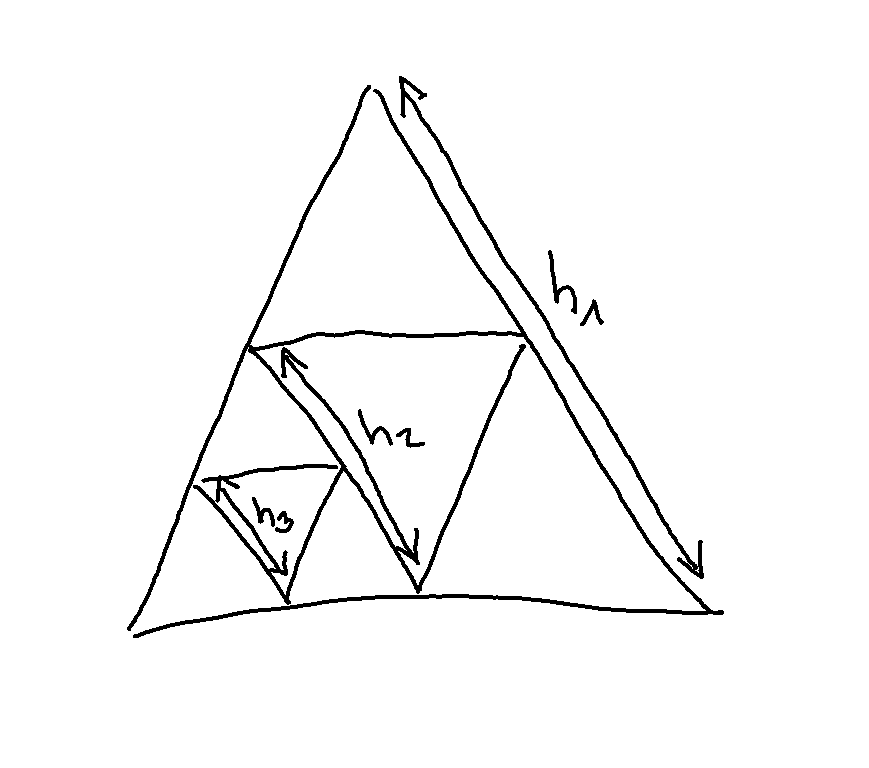
\includegraphics[width=0.75\textwidth]{pics/Sketch3.png}
				\caption{Beispielhafte Verfeinerung der Triangulierung mit einhergehender Konvergenz des Familienparameters}
				\label{AbbFamilienparameterKonvergenz}
			\end{center}
		\end{figure}
	\end{enumerate}
\end{definition}

\begin{theorem}\label{theorem4.16}
	Für eine formreguläre Familie von Finiten-Elementen $(K,V,\Sigma)$, alle affin-äquivalent zu $(\hat{K},\hat{V},\hat{\Sigma})$, ist die Abschätzung
	\begin{align*}
		\big| v-I_K v\big|\leq\tilde{c}\cdot\big(\meas(K)\big)^{\frac{1}{q}-\frac{1}{p}}\cdot h_K^{r+1-m}\cdot|v|_{r+1,p,K}
	\end{align*}
	erfüllt unter den Voraussetzungen von Theorem \ref{theorem4.14}. Außerdem gilt die Abschätzung dann für die Norm anstelle der Semi-Norm:
	\begin{align*}
		\big\Vert v-I_K v\big\Vert\leq\tilde{c}\cdot\big(\meas(K)\big)^{\frac{1}{q}-\frac{1}{p}}\cdot h_K^{r+1-m}\cdot|v|_{r+1,p,K}
	\end{align*}
\end{theorem}

\begin{theorem}\label{theorem4.17}
	Sei $V:=H_0^1(\Omega)$, $V_h\subseteq V$ ein Raum von Finiten Elementen auf $\T_h$ (gehörend zu einer formregulären Familie)  und seien $(K,V,\Sigma)$ affin-äquivalent zu $(\hat{K},\hat{V},\hat{\Sigma})$.\\
	Weiterhin sei $a$ eine koerzive, stetige Bilinearform auf $V$ und $l$ eine stetige Linearform auf $V$.
	Außerdem seien $u\in V$ und $u_h\in V_h$ die 	eindeutigen Lösungen des Variationsproblems auf $V$ bzw. $V_h$.
	Zusätzlich seien $\hat{N}_i\in\hat{\Sigma}$ stetig auf $H^{r+1}(\hat{K})$ und $P_r(\hat{K})\subseteq\hat{V}\subseteq H^1(\hat{K})$\\
	Dann gibt es eine Konstante $c$, unabhängig von $h$ so, dass
	\begin{align*}
		\Vert u-u_h\Vert_{1,2,\Omega}\leq c\cdot h^r\cdot|u|_{r+1,2,\Omega}
	\end{align*}
	unter der Voraussetzung, dass
	\begin{align*}
		u\in H^1_0(\Omega)\cap H^{r+1}(\Omega).
	\end{align*}
\end{theorem}

\begin{proof}
	Céa's Lemma \ref{theorem2.2CeasLemma} liefert
	\begin{align*}
		\Vert u-u_h\Vert_{1,2,\Omega}&\leq c\cdot \inf\limits_{v_h\in V_h}\Vert u-v_h\Vert_{1,2,\Omega}
		\leq c\cdot\Vert u-I_h u\Vert_{1,2,\Omega}
	\end{align*}
	Mit Theorem \ref{theorem4.16} folgt mit $m=1,p=q=2$ dann die Lokalisierungseigenschaft
	\begin{align*}
		\big(I_h v\big)\big|_K&=I_K\big(v|_K\big)\\
		\implies
		\big\Vert u-I_K u\big\Vert_{1,2,K}&\leq c\cdot h_K^r\cdot|u|_{r+1,2,K}\\
		\implies
		\big\Vert u-I_h u\big\Vert^2_{1,2,\Omega}
		&=\sum\limits_{K\in\T_h}\big\Vert u-I_h u\big\Vert^2_{1,2,K}\\
		&=\sum\limits_{K\in\T_h}\big\Vert u-I_K u\big\Vert^2_{1,2,K}\\
		&\leq
		c\cdot\sum\limits_{K\in\T_h}\underbrace{h_K^{2\cdot r}}_{\leq h^{2\cdot r}}\cdot|u|^2_{r+1,2,K}\\
		&\leq c\cdot h^{2\cdot r}\cdot\underbrace{\sum\limits_{K\in\T_h}|u|^2_{r+1,2,K}}_{=|u|^2_{r+1,2,\Omega}}\\
		&=c\cdot h^{2\cdot r}\cdot|u|^2_{r+1,2,\Omega}
	\end{align*}
\end{proof}

\begin{theorem}\label{theorem4.18}
	Zusätzlich zu den Voraussetzungen von Theorem \ref{theorem4.17} nehmen wir hier noch an, dass das Problem
	\begin{align*}
		\text{Finde }\varphi\in V\text{ so, dass }a(v,\varphi)=(g,v)~\forall v\in V.
	\end{align*}
	%provides?
	für alle $g\in L^2(\Omega)$ eine eindeutige Lösung $\varphi_g\in H^2(\Omega)$ hat, die
	\begin{align*}
		\Vert\varphi_g\Vert_{2,2,\Omega}\leq c\cdot\Vert g\Vert_{0,2,\Omega}
	\end{align*}
	erfüllt. Dann existiert eine Konstante $c$, unabhängig von $h$ so, dass
	\begin{align*}
		\Vert u-u_h\Vert_{0,2,\Omega}\leq c\cdot h^{r+1}\cdot|u|_{r+1,2,\Omega}
	\end{align*}
	falls $u\in H^{r+1}(\Omega)$.
\end{theorem}

\begin{proof}
	Nutze Theorem \ref{theorem2.3AubinNitscheDualitaetsargument} mit $H=L^2(\Omega),V=H_0^1(\Omega)$:
	\begin{align*}
		\Vert u-u_h\Vert_{0,2,\Omega}
		&\leq c\cdot\underbrace{\Vert u-u_h\Vert_{1,2,\Omega}}_{\leq c \cdot h^r\cdot|u|_{r+1,2,\Omega}}\cdot\sup\limits_{\begin{subarray}{c}g\in L^2(\Omega)\\\Vert g\Vert_{0,2,\Omega}=1\end{subarray}}\inf\limits_{v_h\in V_h}\Vert\varphi_g-v_h\Vert_{1,2,\Omega}
	\end{align*}
	\begin{align*}
		\implies
		\inf\limits_{v_h\in V_h}\Vert\varphi_g-v_h\Vert_{1,2,\Omega}
		&\leq\big\Vert\varphi_g -I_h\varphi_g\big\Vert_{1,2,\Omega}\\
		&\leq c\cdot h\cdot|\varphi_g|_{2,2,\Omega}\\
		&\leq c\cdot h\cdot\underbrace{\Vert g\Vert_{0,2,\Omega}}_{=1}
	\end{align*}
	\begin{align*}
		\implies
		\sup\limits_{\begin{subarray}{c}g\in L^2(\Omega)\\\Vert g\Vert_{0,2,\Omega}=1\end{subarray}}\inf\limits_{v_h\in V_h}\Vert\varphi_g-v_h\Vert_{1,2,\Omega}
		\leq c\cdot h
	\end{align*}
\end{proof}

Diese Abschätzungen ist eine \textbf{a priori Abschätzung}, d.h. man kann ohne Berechnungen Aussagen machen.

\begin{lemma}[Inverse Abschätzung]\label{lemma4.19InverseAbschaetzung}\enter
Sei $\lbrace V_h\rbrace$ eine Familie von affin-äquivalenten, formregulären Finiten-Elementen.\\
Dann gibt es eine konstante $c$, unabhängig von $h$, so, dass
	\begin{align*}
		|w_h|_{1,2,K}\leq c\cdot h^{-1}_K\cdot\Vert w_h\Vert_{0,2,K}\qquad\forall w\in V_h
	\end{align*}
	Global erhalten wir
	\begin{align*}
		|w_h|_{1,2,\Omega}\leq c\cdot h^{-1}_{\min}\cdot\Vert w_h\Vert_{0,2,\Omega}\qquad\forall w\in V_h
	\end{align*}
	wobei $h_{\min}:=\min\limits_{K\in\T_h} h_K$
\end{lemma}

\begin{proof}
	\begin{align*}
		|w_h|_{1,2,K}
		\overset{\ref{theorem4.9}}&{\leq}
		c\cdot\underbrace{\Vert B_K^{-1}\Vert^1}_{\leq h_K^{-1}}\cdot\big|\det(B_K)\big|^{\frac{1}{2}}\cdot\big|\underbrace{\hat{w}}_{=w_h\circ F_K}\big|_{1,2,\hat{K}}\\
		|\hat{w}_h|_{1,2,\hat{K}}
		&\leq \Vert\hat{w}\Vert_{1,2,\hat{K}}
		\stackrel{(\ast)}{\leq}
		c\cdot\Vert\hat{w}_h\Vert_{0,2,\hat{K}}\\
		\implies
		|w_h|_{1,2,K}
		&\leq c\cdot h_K^{-1}\cdot\big|\det(B_K)\big|^{\frac{1}{2}}\cdot\Vert\hat{w}_h\Vert_{0,2,\hat{K}}\\
		&\leq c\cdot h_K^{-1}\cdot\big|\det(B_K)\big|^{\frac{1}{2}}\cdot\underbrace{\Vert B_K\Vert^0}_{=1}\cdot\big|\det(B_K)\big|^{-\frac{1}{2}}\cdot\Vert w_h\Vert_{0,2,K}\\
		&= c\cdot h_K^{-1}\cdot\Vert w_h\Vert_{0,2,K}
	\end{align*}
	Bei ($\ast$) wird die Normäquivalenz auf endlichen-dimensionalen $\hat{V}$ benutzt.
\end{proof}
	% This work is licensed under the Creative Commons
% Attribution-NonCommercial-ShareAlike 4.0 International License. To view a copy
% of this license, visit http://creativecommons.org/licenses/by-nc-sa/4.0/ or
% send a letter to Creative Commons, PO Box 1866, Mountain View, CA 94042, USA.
% vim: set noexpandtab:

\section{Nichtkonforme Methoden} %5
\textbf{Nichtkonform} bedeutet: $V_h\not\subseteq V$\\
\textbf{Konform} bedeutet: $V_h\subseteq V$\\
Warum nichtkonforme Methoden?
\begin{enumerate}[label=(\roman*)]
	\item Probleme höherer Ordnung, z. B. von 4. Ordnung
	\begin{align*}
		V=H^2(\Omega)\qquad\qquad%\\
		\text{Konformität}\implies V_h\subseteq C^1
	\end{align*}
\item Skizze für Zerlegung des Gebietes in vier Teilgebiete, siehe Abbildung \ref{AbbNonconformingMethods}
	\begin{figure}[!ht]
		\begin{center}
			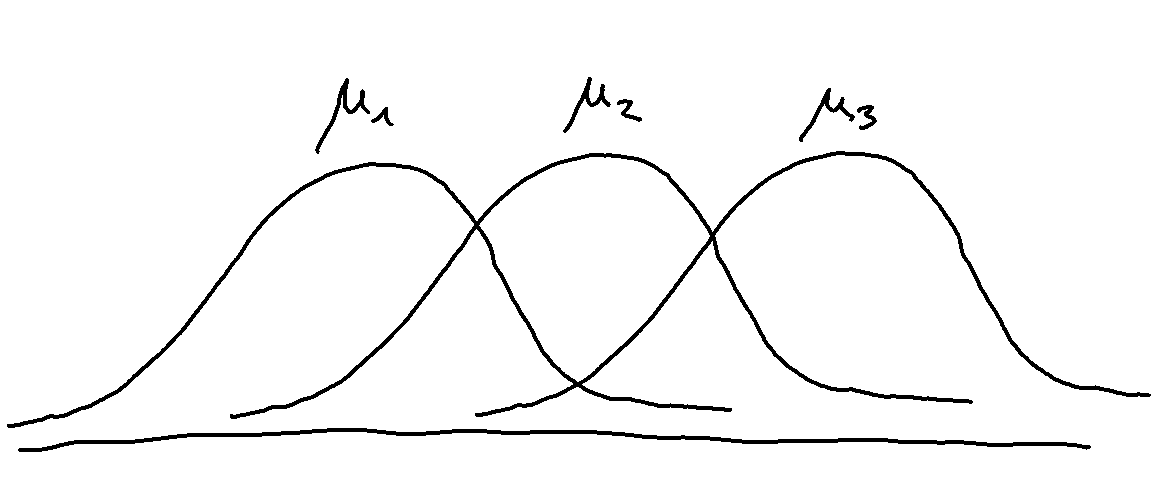
\includegraphics[width=0.75\textwidth]{pics/Sketch5.png}
			\caption{links: konformes $P_1$, rechts nichtkonformes $P_1$}
			\label{AbbNonconformingMethods}
		\end{center}
	\end{figure}
	\item Probleme mit Restriktionen/ Einschränkungen
\end{enumerate}

\subsection{Das nichtkonforme \texorpdfstring{$P_1$}{P\_1}-Element}
Alternative Bezeichnung: Crouzeix-Raviart, 1973\\
Definition lokaler Finite-Elemente $(K,V,\Sigma)$
\begin{align*}
	K&=\text{Dreieck oder Tetraeder}\\
	V&=P_1(K)=\spann\{1,x,y\}\text{ oder }\spann\{1,x,y,z\}\\
	\Sigma&=\big\{N_1,N_2,N_3\big\}\text{ oder }\big\lbrace N_1,N_2,N_3,N_4\big\rbrace\\
	N_i&:\text{ Integral-Mittelwert der Funktionen auf Kanten}\\
	&\text{(äquivalente Alternative: Funktionswerte auf den Mittelpunkten)}
\end{align*}

\begin{beisp}\enter
	\begin{figure}[!ht]
		\begin{center}
			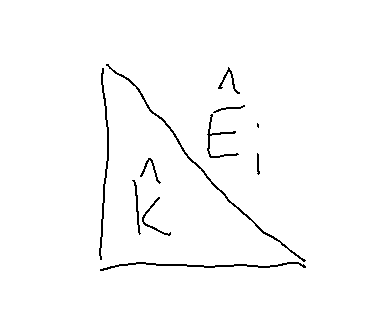
\includegraphics[width=0.25\textwidth]{pics/Sketch6.png}
			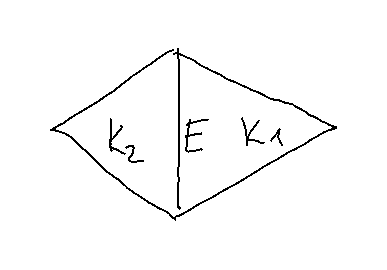
\includegraphics[width=0.25\textwidth]{pics/Sketch7.png}
			\caption{links Referenzdreieck mit Außenkante, rechts Dreiecke mit Innenkante}
			\label{AbbKantentypen}
		\end{center}
	\end{figure}
	\begin{align*}
		\hat{N}_i(\hat{v})=\frac{1}{|\hat{E}_i|}\cdot\int\limits_{\hat{E}_i}\hat{v}\d\gamma
	\end{align*}
\end{beisp}

Der Raum der Finiten-Elemente $V_h$ ist hierbei
\begin{align*}
	V_h=\left\lbrace v\in L^2(\Omega):
	\begin{array}{l}
		v|_K\in P_1(K), \\
		\int\limits_E [v]_E\d\gamma=0~\forall
		\text{ inneren Kanten $E$},\\
		\frac{1}{|E|}\cdot\int\limits_E v\d\gamma=0~\forall\text{ äußeren Kanten }E
	\end{array}
	\right\rbrace
\end{align*}
Hierbei ist $[v]_E$ der Sprung von $v$ über Kanten $E$.\\
\ul{Beobachtung}: Raum der stetigen, stückweise linearen Funktionen ist eine Teilmenge von $V_h$ mit Nullrandbedingungen (d.h. die Funktionen verschwinden auf dem Rand). Es folgt
\begin{align*}
	\inf\limits_{v_h\in V_h}\big\Vert u-v_h\big\Vert_{0,2,\Omega}
	\leq\inf\limits_{w_h\in S_{h,0}^{1,0}}\big\Vert u-w_h\big\Vert_{0,2,\Omega}
	\leq c\cdot h^2\cdot|u|_{2,2,\Omega}
\end{align*}
Wegen $V_h\not\subseteq V$ brauchen wir die Verallgemeinerung von $|\cdot|_{1,2,\Omega}$ für $v\in V=H^1_0(\Omega)$:
\begin{align*}
	|v|_{1,2,\Omega}^2
	&=\sum\limits_{K\in\T_h}|v|^2_{1,2,K}
	=\sum\limits_{K\in\T_h}\Big| v|_K\Big|^2_{1,2,K}
\end{align*}
Definiere
\begin{align*}
	|v|_{1,h}:=\left(\sum\limits_{K\in\T_h}|v|^2_{1,2,K}\right)^{\frac{1}{2}}
\end{align*}
Ist $|\cdot|_{1,h}$ eine Norm auf $V_h$? Es reicht die Null-Eigenschaft zu prüfen:
\begin{align*}
	|v_{1,h}|=0\implies v|_K=\text{konst.}
	\stackrel{\int\limits_E[v]_E\d\gamma=0}{\implies}
	v=\text{konst. auf }\Omega
	\stackrel{\int\limits_{E\in\Gamma} v\d\gamma=0}{\implies}
	v\equiv 0
\end{align*}
Folglich ist es wirklich eine Norm. Es gilt außerdem:
\begin{align*}
	\inf\limits_{v_h\in V_h}\big|u-v_h\big|_{1,h}
	\leq\inf\limits_{w_h\in S_{h,0}^{1,0}}\underbrace{\big|u-w_h\big|_{1,h}}_{|u-w_h|_{1,2}}
	\leq c\cdot h\cdot|u|_{2,2}
\end{align*}

\subsection{Abstraktes Framework}
Wir betrachten unser Modellproblem:
\begin{align*}
	\left\lbrace\begin{array}{rl}
		-\Delta u=f&\text{ in }\Omega\\
		u=0& \text{ auf }\Gamma=\partial\Omega
	\end{array}\right.
\end{align*}
Variationsformulierung: Finde $u\in V=H_0^1(\Omega)$ so, dass
\begin{align*}
	\underbrace{\int\limits_\Omega\nabla u\cdot\nabla v\d x}_{=:a(u,v)}=\underbrace{\int\limits_\Omega f\cdot v\d x}_{=:(f,v)}\qquad\forall v\in V
\end{align*}
Schwierigkeit: $a$ ist nicht definiert für alle Funktionen aus $V_h$. Setze
\begin{align*}
	a_h(v_h,w_h):=\sum\limits_{K\in\mathcal{T}_h}\int\limits_K\nabla v_h\cdot\underbrace{\nabla w_h}_{=\nabla(w_h|_K)}\d x
\end{align*}
Diskretes Problem: Finde $u_h\in V_h$ so, dass
\begin{align*}
	a_h(u_h,v_h)=(f,v_h)\qquad\forall v_h\in V_h
\end{align*}

\textbf{Annahmen:}
\begin{itemize}
	\item $V$ sei ein Hilbertraum
	\item $V_h$ sei ein diskreter Finite-Elemente-Raum mit Norm $\Vert\cdot\Vert_h$
	\item $a\colon V\times V\to\R$ sei ein stetige, $V$-elliptische Bilinearform
	\item $f\colon V\to\R$ sei linear und stetig
\end{itemize}
Dann sagt Lax-Milgram \ref{theorem2.1LaxMilgram}: Es existiert genau ein $u\in V$, welches das Problem löst.\nl
\textbf{Weitere Annahmen:}
\begin{itemize}
	\item $a_h$ sei eine Bilinearform auf $V+ V_h$ %kein Plan warum er hier $V+V_h$ schreibt. Ich ziehe das mal konsequent durch.
	\item $a_h$ sei \textbf{gleichmäßig stetig auf $V+ V_h$}, d. h.
	\begin{align*}
		\exists M>0\text{ unabhängig von }h:\big|a_h(u,v)\big|\leq M\cdot\Vert u\Vert_h\cdot\Vert v\Vert_h\qquad\forall u,v\in V+ V_h
	\end{align*}
	\item $f_h\colon V_h + V\to\R$ sei linear und stetig % orig: \cup, aber warum, wir haben doch überall + ?!
	\item $a_h$ ist \textbf{gleichmäßig $V_h$-elliptisch}, d.h.
	\begin{align*}
		\alpha\cdot\Vert v_h\Vert^2_h\leq a_h(v_h,v_h)\qquad\forall v_h\in V_h
	\end{align*}
	wobei $\alpha$ unabhängig von $v_h$ und $h$ ist.
\end{itemize}
Dann sagt Lax-Milgram \ref{theorem2.1LaxMilgram}: Es existiert genau ein $u_h\in V_h$, welches das Problem löst. Welcher Zusammenhang besteht nun zwischen $u$ und $u_h$?

\begin{theorem}[Zweites Lemma von Strang]\label{theorem5.1ZweitesLemmaStrang}\enter
	Sei $\lbrace V_h\rbrace$ eine Familie von (nichtkonformen) Finiten-Elementen-Räumen. Bezeichne $u$ und $u_h$ die schwache bzw. die diskrete Lösung. Dann gilt:
	\begin{align*}
		\big\Vert u-u_h\big\Vert_h\leq\left(1+\frac{M}{\alpha}\right)\cdot\inf\limits_{v_h\in V_h}\big\Vert u-v_h\big\Vert_h
		+\frac{1}{\alpha}\cdot\sup\limits_{z_h\in V_h}\frac{a_h(u,z_h)-f_h(z_h)}{\Vert z_h\Vert_h}
	\end{align*}
	Hierbei ist erste Summand auf der rechten Seite der Approximationsfehler und der zweite Term der Konsistenzfehler.
\end{theorem}

\begin{bemerkung}
	konforme Methode: $V_h\subseteq V,~a_h=a,f_h=f$ und damit:
	\begin{align*}
		a_h(u,z_h)-f_h(z_h)=a(u_h,z_h)-f(z_h)=0\text{ wegen } z_h\in V_h\subseteq V
	\end{align*}
	Folglich gibt es im Fall der konformen Methode keinen Konsistenzfehler.
\end{bemerkung}

\begin{proof}
	Sei $v_h\in V_h$ beliebig, $w_h\coloneqq v_h-u_h$. Dann gilt:
	\begin{align*}
		α \norm{v_h-u_h}_h^2
		&\leq a_h\big(v_h-u_h,v_h-u_h\big) = a_h\big(v_h-u_h, w_h\big)\\
		&=a_h\big(v_h,w_h\big)-\underbrace{a_h\big(u_h,w_h\big)}_{=f_h(w_h)}\\
		&=a_h\big(v_h-u,w_h\big)+a_h\big(u,w_h\big)-f_h\big(w_h\big)\cdot\frac{\Vert w_h\Vert_h}{\Vert w_h\Vert_h}\\
		&\leq M\cdot\big\Vert v_h-u\big\Vert_h\cdot\big\Vert w_h\big\Vert_h+\Vert w_h\Vert_h\cdot\sup\limits_{z_h\in V_h}\frac{a_h\big(u,z_h\big)-f_h\big(z_h\big)}{\Vert z_h\Vert_h}\\
		\implies
		\underbrace{\norm{w_h}_h}_{=\norm{v_h-u_h}_h}
		&\leq\frac M{α} · \norm{v_h-u}_h
		+ \frac1{α} · \sup_{z_h ∈ V_h} \frac{a_h\big(u,z_h\big)-f_h\big(z_h\big)}{\norm{z_h}_h}
	\end{align*}
	Mit der Dreicksungleichung folgt:
	\begin{align*}
		\norm{u-u_h}_h
		&\leq \norm{u-v_h}_h + \norm{v_h-u_h}_h\\
		&\leq\left(1+\frac{M}{\alpha}\right)\cdot\Vert u-v_h\Vert_h+\frac{1}{\alpha}\cdot\sup\limits_{z_h\in V_h}\frac{a_h\big(u,z_h\big)-f_h\big(z_h\big)}{\Vert z_h\Vert_h}
	\end{align*}
	Bilden des Infimums $\inf\limits_{v_h\in V_h}$ liefert die Behauptung.
\end{proof}

\subsection{Überprüfen der Voraussetzungen für das Poisson-Problem}
\begin{align*}
	a_h(v_h,w_h)&=\sum\limits_{K\in\T_h}\int\limits_K\nabla v_h\cdot\nabla w_h\d x\\
	f_h(v_h)&=\sum\limits_{K\in\T_h}\int\limits_K f\cdot v_h\d x\\
	\Vert v\Vert_h&=\left(\sum\limits_{K\in\T_h}|v|_{1,2,K}\right)^{\frac{1}{2}}
\end{align*}
$\Vert\cdot\Vert_h$ ist eine Norm auf $V+ V_h$.\\
Gleichmäßige Stetigkeit von $a_h$ auf $V+ V_h$: Seien $v,w\in V\cup V_h$. Dann gilt:
\begin{align*}
	\big|a_h(v,w)\big|
	&=\left|\sum\limits_{K\in\T_h}\int\limits_K\nabla v\cdot\nabla w\d x\right|\\
	\overset{\text{CS}}&\leq
	\sum\limits_{K\in\T_h}|v|_{1,2,K}\cdot |w|_{1,2,K}\\
	\overset{\text{CS}}&\leq
	\left(\sum\limits_{K\in\T_h} |v|_{1,2,K}^2\right)^{\frac{1}{2}}\cdot\left(\sum\limits_{K\in\T_h}|w|_{1,2,K}^2\right)^{\frac{1}{2}}\\
	&=\Vert v\Vert_h\cdot\Vert w\Vert_h \quad
	(\implies M=1)
\end{align*}
Gleichmäßige $V_h$-Elliptizität von $a_h$ auf $V_h$: Sei $v_h\in V_h$ beliebig. Dann gilt:
\begin{align*}
	a_h(v_h,v_h)
	&=\sum\limits_{K\in\T_h}\int\limits_K\nabla v_h\cdot\nabla v_h\d x
	=\sum\limits_{K\in\T_h}|v_h|^2_{1,2,K}
	=\Vert v_h\Vert^2_h \quad
	(\implies\alpha=1)
\end{align*}
Stetigkeit von $f_h$ auf $V_h$:
\begin{align*}
	\big|f_h(v_h)\big|
	&=\left|\sum\limits_{K\in\T_h}\int\limits_K f\cdot v_h\d x\right|
	\overset{\text{}}\leq
	\sum\limits_{K\in\T_h}\Vert f \Vert_{0,2,K}\cdot\Vert v_h\Vert_{0,2,K}
	\overset{\text{}}\leq
	\Vert f\Vert_{0,2,\Omega}\cdot\Vert v_h\Vert_{0,2,\Omega}
\end{align*}
Auf $V_h$ (endlich-dimensionaler Raum) sind die Normen $\Vert\cdot\Vert_h$ und $\Vert\cdot\Vert_{0,2,\Omega}$ äquivalent:
\begin{align*}
	\implies
	\big|f_h(v_h)\big|
	\leq
	c_h\cdot\Vert f\Vert_{0,2,\Omega}\cdot\Vert v_h\Vert_h
\end{align*}

\subsection{Fehlerabschätzung} %5.4
Bisher:
\begin{align*}
	\Vert u-u_h\Vert_h
	&\leq
	2\cdot\underbrace{\inf\limits_{v_h\in V_h}\Vert u-v_h\Vert_h}_{\leq c\cdot h\cdot |u|_{2,2}}+1\cdot\underbrace{\sup\limits_{z_h\in V_h}\frac{a_h(u,z_h)-f_h(z_h)}{\Vert z_h\Vert_h}}_{\leq?}
\end{align*}
Sei $f\in L^2(\Omega)$ und $u\in H^2(\Omega)$. Dann:
\begin{align*}
	-\laplace u=f \text{ im $L^2$-Sinn auf jedem } K ∈ \T_h
\end{align*}
Sei nun $z_h\in V_h$ beliebig. Dann gilt:
\begin{align*}
	Σ_{K∈\T_h}∫\limits_K-\laplace u · z_h\d x
	&=Σ_{K∈\T_h}∫\limits_K f · z_h\d x\\
	Σ_{K∈\T_h}∫\limits_K-\laplace u · z_h\d x
	\overset{\text{part. Int.}}&=
	Σ_{K∈\T_h}\left(∫\limits_K∇ u · ∇ z_h\d x-∫\limits_{\Rand K}\underbrace{\frac{∂ u}{∂ n_K}}_{=∇ u · n_K}z_h\d γ \right)\\
	\implies L_h(z_h)
	&\coloneqq a_h(u,z_h)-f_h(z_h)\\
	&=Σ_{K∈\T_h}∫\limits_{\Rand K}\frac{∂ u}{∂ n_K}z_h\d γ \\
	&=Σ_{E}∫\limits_E\underbrace{\left[\frac{∂ u}{∂ u_E}z_h\right]_E}_{=\frac{∂ u}{∂ u_E}[z_h]_E}\d γ \\
	&=Σ_E∫\limits_E\frac{∂ u}{∂ u_E}[z_h]_E\d γ \\
	\text{wobei } [v]_E &\coloneqq v|_{K_1}-v|_{K_2}
\end{align*}
\begin{figure}[!ht]
	\begin{center}
		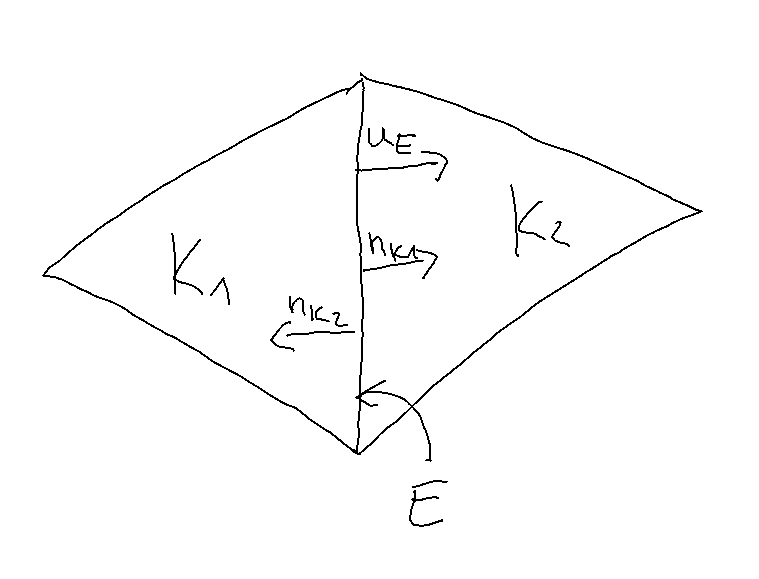
\includegraphics[width=0.75\textwidth]{pics/Sketch8.png}
		\caption{Skizze der Normalen an Kante zwischen zwei Dreiecken}
		\label{AbbNormalvectors}
	\end{center}
\end{figure}
Seien $\overline{z}_h$ und $\overline{\frac{\partial u}{\partial u_E}}$ die konstanten Integral-Mittelwerte von $z_h$ und $\frac{\partial u}{\partial u_E}$ auf jedem $E$, formal:
\begin{align*}
	\overline{z}_h|_E
	:&=\frac{1}{|E|}\cdot\int\limits_E z_h\d\gamma,\qquad\left.\overline{\frac{\partial u}{\partial u_E}}\right|_E \coloneqq \frac{1}{|E|}\cdot\int\limits_E \frac{\partial u}{\partial u_E}\d\gamma
\end{align*}
Mit
\begin{align*}
	\int\limits_E[z_h]_E\d\gamma=0\text{ wegen }z_h\in V_h
\end{align*}
und da $\overline{\frac{\partial u}{\partial u_E}}$ eine Konstante ist
folgt
\begin{align*}
	\int\limits_E\frac{\partial u}{\partial u_E}[z_h]_E\d\gamma
	&=\int\limits_E\left(\frac{\partial u}{\partial u_E}-\overline{\frac{\partial u}{\partial u_E}}\right)[z_h]_E\d\gamma
	=\int\limits_E\left(\frac{\partial u}{\partial u_E}-\overline{\frac{\partial u}{\partial u_E}}\right)[z_h-\overline{z}_h]_E\d\gamma\\
	\implies
	L_h(z_h)
	&=\sum\limits_{K\in\T_h}\sum\limits_{E\subseteq\partial K}\int\limits_E\left(\frac{\partial u}{\partial u_E}-\overline{\frac{\partial u}{\partial u_E}}\right)\big[z_h-\overline{z}_h\big]_E\d\gamma\\
	\overset{\text{CS}}&\leq
	\sum\limits_{K\in\T_h}\sum\limits_{E\subseteq\partial K}\left\Vert\frac{\partial u}{\partial u_E}-\overline{\frac{\partial u}{\partial u_E}}\right\Vert_{0,2,E}\cdot\Vert z_h-\overline{z}_h\Vert_{0,2,E}
\end{align*}
Berechne nun für die Differenz: $z_h-\overline{z}_h$:
\begin{align*}
	\big\Vert z_h-\overline{z}_h\big\Vert_{0,2,E}
	&\leq
	c\cdot\underbrace{\big\Vert B_E^{-1}\big\Vert^0}_{=1}\cdot{\underbrace{\big|\det(B_E)\big|}_{=h_E}}^{\frac{1}{2}}\cdot\big\Vert \underbrace{\hat{z}_h-		\hat{\overline{z}}_h}_{=\widehat{z_h-\overline{z}_h}}\big\Vert_{0,2,\hat{E}}\\
	&\leq
	c\cdot h_E^{\frac{1}{2}}\cdot\big\Vert\widehat{z_h-\overline{z}_h}\big\Vert_{0,2,\hat{E}}
\end{align*}
Der Operator
\begin{align*}
	L\colon H^1(\hat{K})\to L_2(\hat{E}),\qquad\hat{v}\mapsto\left(\hat{v}-\overline{\hat{v}}\right)|_{\hat{E}}
	\mit \overline{\hat{v}}=\frac{1}{|\hat{E}|}\cdot\int\limits_{\hat{E}}\hat{v}\d\gamma
\end{align*}
ist linear und stetig. Folglich gilt:
\begin{align*}
	\big\Vert L(\hat{v})\big\Vert_{0,2,\hat{E}}
	&=\big\Vert\hat{v}-\overline{\hat{v}}\big\Vert_{0,2,\hat{E}}
	\leq
	\underbrace{\Vert\hat{v}\Vert_{0,2,\hat{E}}}_{\stackrel{\text{Spursatz}}{\leq} c\cdot\Vert\hat{v}\Vert_{1,2,\hat{K}}}+\big\Vert\overline{\hat{v}}\big		\Vert_{0,2,\hat{E}}\\
	\big\Vert\overline{\hat{v}}\big\Vert^2_{0,2,\hat{E}}
	&=
	\int\limits_{\hat{E}}\big|\overline{\hat{v}}\big|^2\d\gamma \\
	&=
	\left(\frac{1}{|\hat{E}|}\cdot\int\limits_{\hat{E}}\hat{v}\d\gamma\right)^2\cdot|\hat{E}|\\
	&\leq
	\frac{1}{|\hat{E}|^2}\cdot\Big(\underbrace{\Vert1\Vert_{0,2,\hat{E}}}_{=|\hat{E}|^{\frac{1}{2}}}\cdot\Vert\hat{v}\Vert_{0,2,\hat{E}}\Big)^2\cdot|\hat{E}|\\
	&=\Vert\hat{v}\Vert^2_{0,2,\hat{E}}\\
	&\leq c\cdot\Vert\hat{v}\Vert_{1,2,\hat{K}}
\end{align*}
Somit:
\begin{align*}
	\implies
	\big\Vert L(\hat{v})\big\Vert_{0,2,\hat{E}}
	&\leq c\cdot\Vert\hat{v}\Vert_{1,2,\hat{K}}
\end{align*}
Außerdem
\begin{align*}
	%\implies
	L(\hat{w})&=0\qquad\forall\hat{w}\in P_0(\hat{K})\\
	\overset{\text{Bramble-Hilbert}}{\implies}
	\big\Vert L(\hat{v})\big\Vert_{0,2,\hat{E}}
	&\leq
	c\cdot|\hat{v}|_{1,2,\hat{K}}\\
	\implies
	\big\Vert z_h-\overline{z}_h\big\Vert_{0,2,E}
	&\leq c\cdot h_E^{\frac{1}{2}}\cdot\big|\hat{z}_h\big|_{1,2,\hat{K}}\\
	\overset{\text{transf. zurück}}&{\leq}
	c\cdot h_E^{\frac{1}{2}}\cdot\underbrace{\Vert B_K\Vert^1}_{\sim h_K}\cdot{\underbrace{\big|\det(B_K)\big|}_{\sim h_K^2}}^{-\frac{1}{2}}\cdot|z_h|_{1,2,K}\\
	&\leq
	c\cdot h_E^{\frac{1}{2}}\cdot|z_h|_{1,2,K}
\end{align*}
Auf ähnliche Art und Weise, aber mit wesentlich mehr Aufwand, erhält man auch:
\begin{align*}
	\left\Vert\frac{\partial u}{\partial u_K}-\overline{\frac{\partial u}{\partial u_K}}\right\Vert_{0,2,E}
	&\leq c\cdot h_E^{\frac{1}{2}}\cdot\Vert u\Vert_{2,2,K}
\end{align*}
Nun können wir endlich alle Abschätzungen zusammenbringen und erhalten
\begin{align*}
	\implies
	L_h(z_h)
	&\leq
	\sum\limits_{K\in\T_h}\sum\limits_{E\subseteq\partial K}\left\Vert\frac{\partial u}{\partial u_K}-\overline{\frac{\partial u}{\partial u_K}}\right\Vert_{0,2,E}\cdot\big\Vert z_h-\overline{z}_h\big\Vert_{0,2,E}\\
	&\leq
	c\cdot\sum\limits_{K\in\T_h} h^{\frac{1}{2}}\cdot\Vert u\Vert_{2,2,K}\cdot h^{\frac{1}{2}}\cdot|z_h|_{1,2,K}\\
	&\leq
	c\cdot h\cdot\left(\sum\limits_{K\in\T_h}\Vert u\Vert^2_{1,2,K}\right)^{\frac{1}{2}}\cdot\left(\sum\limits_{K\in\T_h}|z_h|_{1,2,K}^2\right)^{\frac{1}{2}}\\
	&=c\cdot h\cdot \Vert u\Vert_{2,2,\Omega}\cdot\Vert z_h\Vert_h\\
	\implies
	\sup\limits_{z_h\in V_h}\frac{a_h(u, z_h)-f_h(z_h)}{\Vert z_h\Vert_h}
	&\leq c\cdot h\cdot\Vert u\Vert_{2,2,\Omega}
\end{align*}

\begin{theorem}\label{theorem5.2}
	Sei $\lbrace V_h\rbrace$ eine Familie von $P_1$-nichtkonformen Finite-Elemente-Räume, wobei $u_h\in V_h$ das diskrete Problem löst und $u\in V\cap H^2(\Omega)$ die Lösung der schwachen Formulierung ist. Dann gilt:
	\begin{align*}
		\big\Vert u-u_h\big\Vert_h\leq c\cdot h\cdot\Vert u\Vert_{2,2,\Omega}
	\end{align*}
\end{theorem}

\begin{bemerkung}
	Das Dualitätsargument von Aubin und Nietsche kann erweitert werden auf den nichtkonformen Fall. Dabei tauchen zwei neue Terme in der Abschätzung auf.
	\begin{align*}
		\big\Vert u-u_h\big\Vert_{0,2,\Omega}\leq c\cdot h^2\cdot\Vert u\Vert_{2,2,\Omega}
	\end{align*}
\end{bemerkung}
	% This work is licensed under the Creative Commons
% Attribution-NonCommercial-ShareAlike 4.0 International License. To view a copy
% of this license, visit http://creativecommons.org/licenses/by-nc-sa/4.0/ or
% send a letter to Creative Commons, PO Box 1866, Mountain View, CA 94042, USA.
% vim: set noexpandtab:

\section{A posteriori Fehlerabschätzung} %6
Modellproblem: $\Omega\subseteq\R^2,f\in L^2(\Omega)$
\begin{align*}
	\left\lbrace\begin{array}{rl}
		-\Delta u=f &\text{ in }\Omega\\
		u=0 &\text{ auf }\Gamma=\partial\Omega
	\end{array}\right.
\end{align*}
Schwache Formulierung: Finde $u\in H_0^1(\Omega)$ so, dass
\begin{align*}\label{eqSection6P}\tag{$P$}
	\underbrace{\int\limits_\Omega\nabla u\cdot\nabla v\d x}_{=:a(u,v)}=\underbrace{\int\limits_\Omega f\cdot v\d x}_{=:l(v)}\qquad\forall v\in H_0^1(\Omega)
\end{align*}
Konforme Finite-Elemente-Diskretisierung:\\
Sei $\lbrace\T_h\rbrace$ eine Familie von Form-regulären Triangulierungen mit\\ Finiten-Elementen-Räumen $X_h$ von stetigen, stückweise $P_h$-polynomiellen Funktionen\nl
Diskretes Problem: Finde $u\in X_h$ so, dass
\begin{align}\label{eqSection6Ph}\tag{$P_h$}
	a(u_h,v_h)=l(v_h)\qquad\forall v_h\in X_h
\end{align}
Ziel: Finde berechenbare Schranken für den Fehler $u-u_h$ in irgendeiner Norm.

\subsection*{Informelle Definition}
\begin{itemize}
	\item Eine Menge $\eta$ heißt \textbf{(Posteriori-)Fehlerschätzer} $:\gdw\eta$ ist berechenbar aus den Problemdaten und der diskreten Lösung $u_h$.
	\item Ein Fehlerschätzer $\eta$ heißt \textbf{zuverlässig} $:\gdw$ es gibt eine obere Schranke für den globalen Fehler, d.h.
	\begin{align*}
		:\Longleftrightarrow\exists c\in\R:\big\Vert u-u_h\big\Vert_\Omega\leq c\cdot\eta
	\end{align*}
	Zuverlässige Fehlerschätzer sind nützlich um eine gewisse Genauigkeit sicherzustellen.
	\item Ein Fehlerschätzer $\eta$ heißt \textbf{effizient} $:\gdw$ es existiert eine lokale untere Schranke für den Fehler, d.h.
	\begin{align*}
		\eta_{\text{ lokal}}\leq c\cdot\big\Vert u-u_h\big\Vert_{\text{lokal}}+\text{Daten-Oszillation}
	\end{align*}
	Da wir später $f$ durch ein Approximationspolynom ersetzen, kommt ein Fehlerterm hinzu, welchen wir \textbf{Daten-Oszillation} nennen.\\
	Effiziente Fehlerschätzer soll eine Überschätzung der lokalen Verfeinerung verhindern.
\end{itemize}

\subsection*{Residuale Fehlerschätzer}
Aus der Friedrich-Ungleichung \ref{prop1.13FriedrichsUngleichung} folgt:
\begin{align*}
	a(v,v)&\geq\alpha\cdot\Vert v\Vert^2_{1,2,\Omega}\qquad\forall v\in H^1_0(\Omega)\\
	\implies
	\Vert u-u_h\Vert^2_{1,2,\Omega}
	&\leq
	\frac{1}{\alpha}\cdot a\big(u-u_h,u-u_h\big)\\
	\implies
	\Vert u-u_h\Vert_{1,2,\Omega}
	&\leq\frac{1}{\alpha}\cdot a\left(u-u_h,\frac{u-u_h}{\Vert u-u_h\Vert_{1,2,\Omega}}\right)\\
	\implies
	\Vert u-u_h\Vert_{1,2,\Omega}
	&\leq\frac{1}{\alpha}\cdot\sup\limits_{\begin{subarray}{c}v\in H^1_0(\Omega)\\\Vert v\Vert_{1,2,\Omega}=1\end{subarray}}\Big(\underbrace{a(u,v)}_{=l(v)}-a(u_h,v)\Big)
\end{align*}
Andererseits erhalten wir:
\begin{align*}
	\sup\limits_{\begin{subarray}{c}v\in H^1_0(\Omega)\\\Vert v\Vert_{1,2,\Omega}=1\end{subarray}} a(u-u_h,v)
	&\leq
	\sup\limits_{\begin{subarray}{c}v\in H^1_0(\Omega)\\\Vert v\Vert_{1,2,\Omega}=1\end{subarray}}
	\Vert u-u_h\Vert_{1,2,\Omega}\cdot\underbrace{\Vert v\Vert_{1,2,\Omega}}_{=1}
	=\Vert u-u_h\Vert_{1,2,\Omega}\\
\end{align*}
Also bekommen wir die Abschätzungen
\begin{align*}
	\sup\limits_{\begin{subarray}{c}v\in H^1_0(\Omega)\\\Vert v\Vert_{1,2,\Omega}=1\end{subarray}} a(u-u_h,v)
	&\leq
	\Vert u-u_h\Vert_{1,2,\Omega}
	\leq\frac{1}{\alpha}\cdot\sup\limits_{\begin{subarray}{c}v\in H^1_0(\Omega)\\\Vert v\Vert_{1,2,\Omega}=1\end{subarray}} a(u-u_h,v)
\end{align*}
Das bedeutet, dass die Norm $\Vert u_h-u\Vert_{1,2,\Omega}$ äquivalent zu der Operatornorm der linearen Abbildung
\begin{align*}
	R:H^1_0(\Omega)\to\R,\qquad v\mapsto l(v)-a(u_h,v)=a(u-u_h,v)
\end{align*}
ist. Beobachtung: Aus der Galerkin Orthogonalität folgt:
\begin{align*}
	R(v_h)=a(u-u_h,v_h)=0
\end{align*}
Für $v\in H^1_0(\Omega)\mit\Vert v\Vert_{1,2,\Omega}=1$ gilt:
\begin{align*}
	R(v)&=l(v)-a(u_h,v)\\
	&=\int\limits_\Omega f\cdot v\d x-\int\limits_\Omega\nabla u_h\cdot\nabla v\d x\\
	&=\sum\limits_{T\in\T_h}\left(\int\limits_T f\cdot v\d x-\int\limits_T \nabla u_h\cdot\nabla v\d x\right)\\
	&=\sum\limits_{T\in\T_h}\left(\int\limits_T f\cdot v\d x+\int\limits_T\Delta u_h\cdot v\d x-\int\limits_{\partial T}\nabla u_h\cdot u_T\cdot v\d\gamma\right)\\
	&=\sum\limits_{T\in\T_h}\int\limits_T\big(f+\Delta u_h\big)\cdot v\d x
	+\sum\limits_{E\in\mathcal{E}_h}\int\limits_E\big[\nabla u_h\cdot u_E\big]_E\cdot v\d\gamma\\
	\overset{\text{CS}}&\leq
	\sum\limits_{T\in\T_h}\big\Vert f+\Delta u_h\big\Vert_{0,2,T}\cdot\Vert v\Vert_{0,2,T}+\sum\limits_{E\in\mathcal{E}_h}\Big\Vert\big[\nabla u_h\cdot u_E\big]_E\Big\Vert_{0,2,E}\cdot\Vert v\Vert_{0,2,E}
\end{align*}
\begin{align*}
	R(v)
	&=R(v-v_h)\\
	&\leq
	\sum\limits_{T\in\T_h}\big\Vert f+\Delta u_h\big\Vert_{0,2,T}\cdot\Vert v-v_h\Vert_{0,2,T}
	&+\sum\limits_{E\in\mathcal{E}_h}\Big\Vert\big[\nabla u_h\cdot u_E\big]_E\Big\Vert_{0,2,E}\cdot\Vert v-v_h\Vert_{0,2,E}
\end{align*}
,wobei $\mathcal{E}_h$ die Menge aller Kanten ist.
\begin{align*}
	\text{Bester Weg}&: \text{Wähle $v_h$ als Interpolation von } v.\\
	\text{Aber}&: v\text{ ist nur in }H^1\text{ \& die gewöhnliche Interpolation wird nicht funktionieren.}\\
	\text{Lösung}&:\text{Quasi-Interpolation.}\\
	\text{Hier}&: \text{Quasi-Interpolation von Clément}
\end{align*}

\begin{notation}\
	\begin{itemize}
		\item $N_h$ ist die Menge Knoten.
		\item $N_{h,\Omega}$ ist die Menge aller Knoten in $\Omega$.
		\item $\varphi_z\in S^{1,0}_{h,0}$ sei stetig, stückweise lineare Hut-Funktion assoziiert zu $z\in N_h$
		\item $\overline{w}_z:=\inner\left(\bigcup\limits_{\begin{subarray}{c}T\in\T_h\\z\text{ ist Knoten von }T\end{subarray}}\overline{T}\right)$
		\item Für $v\in L^2(w_z)$ definiere die \textbf{$L^2$-Projektion auf Konstanten} durch
		\begin{align*}
			\pi_z (v):=\frac{1}{|w_z|}\cdot\int\limits_{w_z} v\d x
		\end{align*}
		\item Quasi-Interpolation von Clément:
		\begin{align*}
			R_h:H^1_0(\Omega)\to S^{1,0}_{h,0}\subseteq X_h,\qquad
			R_h(v):=\sum\limits_{z\in N_{h,\Omega}}\left(\pi_z(v)\right)\cdot\varphi_z
		\end{align*}
	\end{itemize}
\end{notation}

Als nächstes brauchen wir Abschätzungen für
\begin{align*}
	\big\Vert v-R_h(v)\big\Vert_{0,2,T}\qquad\text{und}\qquad\big\Vert v-R_h(v)\big\Vert_{0,2,E}
\end{align*}
gegen die $H^1$-Normen auf $v$.

\begin{theorem}[skalierter Spursatz]\label{theoremSkalierterSpursatz}\enter
	Sei $T\in\T_h$ und $E$ eine Kante von $T$.\\
	Dann existiert eine Konstante $c$, die nur von der Form-Regularitäts-Konstante abhängt, so dass
	\begin{align*}
		\Vert v\Vert_{0,2,E}\leq c\cdot\left(h_T^{-\frac{1}{2}}\cdot\Vert v\Vert_{0,2,T}+ h_T^{\frac{1}{2}}\cdot|v|_{1,2,T}\right)\qquad\forall v\in H^1(T)
	\end{align*}
\end{theorem}

Der Wert im Knoten $z$ ist
\begin{align*}
	\pi_z (v)=\frac{1}{|w_z|}\cdot\int\limits_{w_z}v\d x
\end{align*}
Es gilt
\begin{align*}
	\Vert v\Vert_{0,2,E}\leq c\cdot\left(h_T^{-\frac{1}{2}}\cdot\Vert v\Vert_{0,2,T}+h_T^{\frac{1}{2}}\cdot|v|_{1,2,T}\right)
\end{align*}

\begin{proof}
	Bezeichne $\hat{T}$ das Referenzdreieck mit Referenzkante $\hat{E}$. Außerdem sei $T$ ein beliebiges Dreieck mit Ecken $(a_1,b_1)$, $(a_2,b_2)$, $(a_3,b_3)$ und Kante $E$.
	Dann ist die Transformation zwischen beiden Dreiecken gegeben durch
	\begin{align*}
		F_T(\hat{x},\hat{y})=\begin{pmatrix}
			x\\y
		\end{pmatrix}
		&=\begin{pmatrix}
			a_1\\ b_1
		\end{pmatrix}
		+\hat{x}\cdot\begin{pmatrix}
			a_2-a_1\\ b_2-b_1
		\end{pmatrix}+
		\hat{y}\cdot\begin{pmatrix}
			a_3-a_1\\ b_3-b_1
		\end{pmatrix}\\
		&=\begin{pmatrix}
			a_1\\ b_1
		\end{pmatrix}
		+\underbrace{\begin{pmatrix}
			a_2-a_1 & a_3-a_1\\
			b_2-b_1 & b_3-b_1
		\end{pmatrix}}_{=:B_T}\cdot\begin{pmatrix}
			\hat{x}\\ \hat{y}
		\end{pmatrix}
	\end{align*}
	Mit
	\begin{align*}
		\varphi\colon[0,1]\to E,\quad\varphi(s):=\begin{pmatrix}
		a_1\\ b_1
		\end{pmatrix}+s\cdot\begin{pmatrix}
		a_2-a_1\\
		b_2-b_1
		\end{pmatrix},\quad
		\big\Vert\dot\varphi(s)\big\Vert=\left\Vert\begin{pmatrix}
		a_2-a_1\\
		b_2-b_1
		\end{pmatrix}\right\Vert=|E|=h_E
	\end{align*}
	folgt
	\begin{align*}
		&\Vert v\Vert_{0,2,E}^2
		=\int\limits_E|v|^2\d\gamma
		=\int\limits_0^1\Big|v\big(\varphi(s)\big)\Big|^2\cdot\big\Vert\dot{\varphi}(s)\big\Vert\d s
		=h_E\cdot\big\Vert\hat{v}\big\Vert_{0,2,\hat{E}}^2\\
	\end{align*}
	Demnach
	\begin{align*}
		&\big\Vert\hat{v}\big\Vert_{0,2,E}^2\\
		\overset{\ref{satz1.7Spursatz}}&\leq
		c\cdot h_E\cdot\Vert\hat{v}\Vert_{1,2,\hat{T}}^2
		=c\cdot h_E\cdot\left(\Vert\hat{v}\Vert_{0,2,\hat{T}}^2+\Vert\hat{v}\Vert_{1,2,\hat{T}}^2\right)\\
		\overset{\ref{theorem4.9}}&\leq
		c\cdot
		\underbrace{h_E}_{\leq h_T}\cdot\Bigg(c\cdot\underbrace{\Vert B_T\Vert^{0\cdot2}}_{=1}\cdot
		\underbrace{\big|\det(B_t)\big|^{-\frac{1}{2}\cdot2}}_{\leq c\cdot h_T^{-2}}\cdot\Vert v\Vert^2_{0,2,T}+c\cdot
		\underbrace{\Vert B_T\Vert^{1\cdot2}}_{\leq c\cdot h_T^2}\cdot
		\underbrace{\big|\det(B_T)\big|^{-\frac{1}{2}\cdot2}}_{c\cdot h^{-2}_T}\cdot|v|^2_{1,2,T}\Bigg)\\
		&\leq
		c\cdot\left(h_T^{-1}\cdot\Vert v\Vert_{0,2,T}^2+h_T\cdot|v|^2_{1,2,T}\right)
	\end{align*}
	% Das ist doch aber noch nicht die Aussage oder ??? Wurzelziehen auf beiden Seiten ergibt doch etwas anderes
\end{proof}

\begin{theorem} %no number?
	Sei $v\in H_0^1(\Omega)$. Dann gibt es zwei Konstanten $c_1,c_2$, die von $h$ und $v$ unabhängig sind, so, dass
	\begin{align*}
		\big\Vert v-R_h(v)\big\Vert_{0,2,T}&\leq c_1\cdot h_T\cdot|v|_{1,2,\tilde{\omega}_T}\\
		\big\Vert v-R_h(v)\big\Vert_{0,2,E}&\leq c_2\cdot h_E^{\frac{1}{2}}\cdot|v|_{1,2,\tilde{\omega}_E}
	\end{align*}
	Hierbei ist
	\begin{align*}
		\overline{\tilde{\omega}_T}:=\bigcup\limits_{\overline{T'}\cap\overline{T}\neq\emptyset}\overline{T'},\qquad
		\overline{\tilde{\omega}_E}:=\bigcup\limits_{\overline{T'}\cap\overline{E}\neq\emptyset}\overline{T'}
	\end{align*}
	\begin{figure}[!ht]
		\begin{center}
			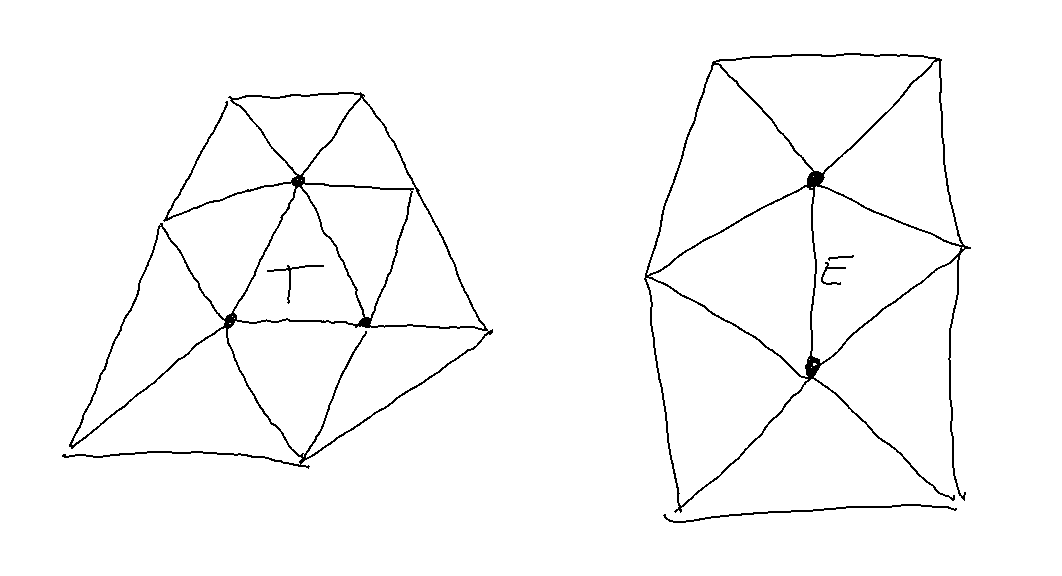
\includegraphics[width=0.75\textwidth]{pics/Sketch9.png}
			\caption{Skizze zur Definition von $\overline{\tilde{\omega}_T}$ (links) und $\overline{\tilde{\omega}_E}$ (rechts)}
			\label{AbbDefinitionUmgebung}
		\end{center}
	\end{figure}
\end{theorem}
% Prof Matthies, nachdem ihm etwas heruntergefallen ist: "Scheiß Schwerkfraft!"

\begin{proof}
	Sei $\mathcal{N}(T)$ die Menge aller Ecken von $T$.
	Sei $\mathcal{N}(E)$ die Menge aller Endpunkte der Kante E. Dann gilt:
	\begin{align*}
		\sum\limits_{z\in\mathcal{N}(T)}\varphi_z|_T=1 \\
		\sum\limits_{z\in\mathcal{N}(E)}\varphi_z|_E=1
	\end{align*}
	\begin{enumerate}[label=\roman*)]
		\item $\begin{aligned}
			\int\limits_{\omega_z}\big(v-\pi_z(v)\big)\d x=0
		\end{aligned}$
		\begin{align*}
			\big\Vert v-\pi_z(v)\big\Vert_{0,2,\omega_z}
			\overset{\ref{korollarPoincareUngleichung}}&\leq
			c_P\cdot\underbrace{\diam(\omega_z)}_{\leq c_3\cdot h_T}\cdot\underbrace{\big|v-\pi_z(v)\big|_{1,2,\omega_z}}_{=|v|_{1,2,\omega_z}}
			=c_4\cdot h_T\cdot|v|_{1,2,\omega_z}
		\end{align*}
		\item
		\begin{align*}
			\big\Vert v-R_h(v)\big\Vert_{0,2,T}=\Bigg\Vert\underbrace{\left(\sum\limits_{z\in\mathcal{N}(T)}\varphi_z\right)}_{=1}\cdot v-\sum\limits_{z\in\mathcal{N}(T)}\pi_z(v)\cdot\varphi_z\Bigg\Vert_{0,2,T}
		\end{align*}
		$T$ hat keine Ecke auf $\partial\Omega=\Gamma$. Also gilt:
		\begin{align*}
			\big\Vert v-R_h(v)\big\Vert_{0,2,T}
			&=\left\Vert\sum\limits_{z\in\mathcal{N}(T)}\big(v-\pi_z(v)\big)\cdot\varphi_z\right\Vert_{0,2,T}\\
			\overset{\text{DU}}&\leq
			\sum\limits_{z\in\mathcal{N}(T)}\Big\Vert\big(v-\pi_z(v)\big)\cdot\underbrace{\varphi_z}_{\in[0,1]}\Big\Vert_{0,2,T}\\
			&\leq
			\sum\limits_{z\in\mathcal{N}(T)}\Big\Vert\big(v-\pi_z(v)\big)\Big\Vert_{0,2,T}\\
			&\leq
			\sum\limits_{z\in\mathcal{N}(T)}\Big\Vert\big(v-\pi_z(v)\big)\Big\Vert_{0,2,\omega_z}\\
			&\leq
			c_4\cdot h_T\cdot\sum\limits_{z\in\mathcal{N}(T)}|v|_{1,2,\omega_z}\\
			&\leq
			3\cdot c_4\cdot h_T\cdot|v|_{1,2,\tilde{\omega}_T}\\
		\end{align*}
		\item $T$ hat mindestens einen Knoten auf $\Gamma$:
		\begin{align*}
			v-R_h(v)
			&=\underbrace{\left(\sum\limits_{z\in\mathcal{N}(T)}\varphi_z\right)}_{=1}\cdot v-\sum\limits_{z\in\mathcal{N}(T)\setminus\Gamma}\pi_z(v)\cdot\varphi_z\\
			&=\sum\limits_{z\in\mathcal{N}(T)}\varphi_z\cdot\big(v-\pi_z(v)\big)+\sum\limits_{z\in\mathcal{N}(T)\cap\Gamma}\big(\pi_z(v)\big)\cdot\varphi_z
		\end{align*}
		Wir berechnen:
		\begin{align*}
			\Big\Vert(\pi_z(v)\big)\cdot\varphi_z\Big\Vert_{0,2,T}
			&\leq
			\big\Vert\underbrace{\pi_z(v)}_{=\text{konst.}}\big\Vert_{0,2,T}
			=\big|\pi_z(v)\big|\cdot|T|^{\frac{1}{2}}
			\leq c_5\cdot h_T\cdot\big|\pi_z(v)\big|
		\end{align*}
		Wenn $z\in\Gamma$, dann ist $E'\subseteq\Gamma$ mit Knoten $z$ und somit:
		\begin{align*}
			\big|\pi_z(v)\big|^2
			&=|E'|^{-1}\cdot\int\limits_{E'}\big|\pi_z(v)\big|^2\d\gamma\\
			&=h_{E'}^{-1}\cdot\big\Vert\pi_z(v)\big\Vert^2_{0,2,E'}\\
			&=h_{E'}^{-1}\cdot\big\Vert\underbrace{v}_{\in H_0^1(\Omega)}-\pi_z(v)\big\Vert^2_{0,2,E'}\\
			&\stackrel{\ref{theoremSkalierterSpursatz}}{\leq}
			c_6^2\cdot h_{E'}^{-1}\cdot\Big(h_{T'}^{-1}\cdot
			\underbrace{\big\Vert v-\pi_z(v)\big\Vert_{0,2,T'}^2}
			_{
			\begin{array}{l}
				\leq\Vert v-\pi_z(v)\Vert^2_{0,2,\omega_z}\\
				\leq c_4^2\cdot h_T^2\cdot|v|^2_{1,2,\omega_z}
			\end{array}}+h_T^{+1}\cdot\underbrace{\big|v-\pi_z(v)\big|^2_{1,2,T'}}_{=|v|^2_{1,2,T'}}\Big)\\
			&\leq
			c_8^2\cdot|v|^2_{1,2,\omega_z} \\
			&\leq
			c_8^2\cdot|v|_{1,2,\tilde{\omega}_T}^2
		\end{align*}
		\begin{align*}
			\implies \Big\Vert\big(\pi_z(v)\big)\cdot\varphi_z\Big\Vert\leq c_9\cdot h_T\cdot|v|_{1,2,\tilde{\omega}_T}
		\end{align*}
		\item  Sei $E$ eine Kante, die keinen Knoten auf $\Gamma$ hat. Dann gilt:
		\begin{align*}
			% the following is not helpful, was just added at the blackboard without use:
			% (in my notes it's in big brackets)
			% \big\Vert v-R_h(v)\big\Vert_{0,2,E}
			% &\leq
			% c\cdot\Big(h_T^{-\frac{1}{2}}\cdot\underbrace{\big\Vert h-R_h(v)\big\Vert_{0,2,T}}_{\leq c\cdot h_T\cdot|v|_{1,2,\tilde{\omega}_T}}+h_T^{\frac{1}{2}}\cdot\underbrace{\big|v-R_h(v)\big|_{1,2,T}}_{=|v|_{1,2,T}}\Big)\\
			\big\Vert v-R_h(v)\big\Vert_{0,2,E}
			&=\Bigg\Vert\sum\limits_{z\in\mathcal{N}(E)}\big(v-\pi_z(v)\big)\cdot\varphi_z\Bigg\Vert_{0,2,E}\\
			&\leq
			\sum\limits_{z\in\mathcal{N}(E)}\big\Vert v-\pi_z(v)\big\Vert_{0,2,E}\\
			&\leq
			c_{10}\cdot\sum\limits_{z\in\mathcal{N}(E)}\Big(h_T^{-\frac{1}{2}}\cdot\underbrace{\big\Vert v-\pi_z(v)\big\Vert_{0,2,T}}_{\leq c\cdot h_T\cdot|v|_{1,2,\omega_z}}+h_T^{\frac{1}{2}}\cdot\underbrace{\big|v-\pi_z(v)\big|_{1,2,T}}_{\leq|v|_{1,2,\omega_z}}\Big)\\
			&\leq
			c\cdot h_E^{\frac{1}{2}}\cdot|v|_{1,2,\tilde{\omega}_E}
		\end{align*}
		\item $E$ hat hat einen Knoten auf dem Rand $Γ$. %Knotenbeschränkung
			Diesen Fall lassen wir hier aus.
			% ist das richtig? Auf jeden Fall sehe ich weder hier noch in meinen Notizen einen Hinweis auf diesen Fall.
		\begin{align*}
			R(v)&=l(v)-a(u_h,v)=l(v-v_h)-a(u_h,v-v_h)\qquad\forall v_h\in X_h\\
			&\leq\sum\limits_{T\in\T_h}\big\Vert f+\Delta u_h\big\Vert_{0,2,T}\cdot\Vert v-v_h\Vert_{0,2,T}\\
			&{}\quad+\sum\limits_{E\in\Sigma_h}\big\Vert[\nabla u_h\cdot n_E]_E\big\Vert_{0,2,E}\cdot\Vert v-v_h\Vert_{0,2,E}
		\end{align*}
		Idee: Nutze $v_h=R_h(v)$.
		\begin{align*}
			R(v)&\leq
			c\cdot\sum\limits_{T\in\T_h}\Big(\left\Vert f+ \Delta u_h\big\Vert_{0,2,T}\cdot h_T\right)\cdot |v|_{1,2,\tilde{\omega}_T}\\
			&\quad+c\cdot\sum\limits_{E\in\Sigma_h}\left(\Big\Vert[\nabla u_h\cdot n_E]_E\Big\Vert_{0,2,E}\cdot h_E^{\frac{1}{2}}\right)\cdot|v|_{1,2,\tilde{\omega}_E}\\
			&\leq
			c\cdot\left(\sum\limits_{T\in\T_h}\big\Vert f+\Delta u_h\big\Vert^2_{0,2,T}\cdot h_T^2\right)^{\frac{1}{2}}\cdot\left(\sum\limits_{T\in\T_h}|v|^2_{1,2,\tilde{\omega}_T}\right)^{\frac{1}{2}}\\
			&\quad+c\cdot\left(\sum\limits_{E\in\Sigma_h}\big\Vert[\nabla u_h\cdot n_E]_E\big\Vert^2_{0,2,E}\cdot h_E\right)\cdot\underbrace{\left(\sum\limits_{E\in\Sigma_h}|v|^2_{1,2,\tilde{\omega}_E}\right)^{\frac{1}{2}}}_{\leq c\cdot |v|_{1,2,\Omega}\text{, $c$ aus Formregulärität}}\\
			&\leq
			c\cdot\underbrace{\left(\sum\limits_{T\in\T_h} h^2_T\cdot\big\Vert f+\Delta u_h\big\Vert^2_{0,2,T}
			+\sum\limits_{E\in\Sigma_h}h_E\cdot\big\Vert[\nabla u_h\cdot n_E]_E\big\Vert^2_{0,2,E}\right)^{\frac{1}{2}}}_{:=\eta}\cdot\Vert v\Vert_{1,2,\Omega}\nl
			&\implies
			\Vert u-u_h\Vert_{1,2,\Omega}
			\leq
			c\cdot\sup\limits_{\begin{subarray}{c}v\in H_0^1(\Omega)\\\Vert v\Vert_{1,2,\Omega}=1\end{subarray}}R(v) \leq c \cdot \eta
		\end{align*}
		Setze
		\begin{align*}
			\eta_T^2&:=h_T^2\cdot\big\Vert f+\Delta u_h\big\Vert^2_{0,2,T}+\frac{1}{2}\cdot\sum\limits_{E\in\Sigma_k\cap\partial T}h_E\cdot\big\Vert[\nabla u_h\cdot n_E]_E\big\Vert^2_{0,2,E}\\
			\eta:&=\left(\sum\limits_{T\in\T_h}\eta^2_T\right)^{\frac{1}{	2}}
		\end{align*}
		$\eta$ ist eine zuverlässige a posteriori Fehler-Abschätzung. \qedhere
	\end{enumerate}
\end{proof}

\begin{definition}[Bubble-Funktion]\enter %no number, but i will give some
	Sei $T\in\T_h$ und $E\in\Sigma_h$. Wir setzen
	\begin{align*}
		\psi_T:=27\cdot\varphi_{z_1}\cdot\varphi_{z_2}\cdot\varphi_{z_3}
	\end{align*}
	wobei $z_1,z_2,z_3$ die Ecken von $T$ sind. Definiere weiterhin
	\begin{align*}
		\psi_E:=4\cdot\varphi_{z_1}\cdot\varphi_{z_2}
	\end{align*}
	wobei $z_1,z_2$ die Enden der Kante $E$ sind.
\end{definition}

\begin{lemma}[Eigenschaften]\ %no lemma in lecture
	\begin{enumerate}[label=\roman*)]
		\item $\begin{aligned}
			\psi_T\in P_3(T)
			\hspace{64pt}
			\psi_E\big|_T\in P_2(T)\qquad\forall\, T\in\omega_E
		\end{aligned}$
		\item $\begin{aligned}
			\psi_T\geq0\text{ in }\overline{T}
			\hspace{61pt}
			\psi_E\geq 0\text{ in }\overline{\omega}_E
		\end{aligned}$
		\item $\begin{aligned}
			\psi_T\equiv0\text{ auf }\partial T
			\hspace{50pt}
			\psi_E\equiv 0\text{ auf }\partial\omega_E
		\end{aligned}$
		\item $\begin{aligned}
			\max\limits_{x\in\overline{T}}\psi_T(x)=1
			\hspace{48pt}
			\max\limits_{x\in\overline{\omega}_E}\psi_E(x)=1
		\end{aligned}$
		\item $\begin{aligned}
			\hspace{120pt}
			\psi_E\in C(\omega_E)
		\end{aligned}$
	\end{enumerate}
\end{lemma}

\begin{theorem}
	Sei $T\in\T_h,E\in\Sigma_h, v\in P_k(T), \sigma\in P_k(E)$. Dann gilt:
	% todo: wäre es nicht sinnvoller align zu nutzen und damit die Nummerierung aus align zu nutzen und jede Zeile mit einem Label zu versehen? Sieht auf jeden Fall besser aus, da keine Leerzeigen dabei sind
	\begin{enumerate}[label=(\arabic*)]
		\item
		\begin{align*}
			c_1\cdot\Vert v\Vert_{0,2,T}
			\leq\left(\int\limits_T\psi_T\cdot v^2(x)\d x\right)^{\frac{1}{2}} \leq\Vert v\Vert_{0,2,T}
		\end{align*}
		\item
		\begin{align*}
			c_2\cdot h_T^{-1}\cdot\big\Vert\psi_T v\big\Vert_{0,2,T}\leq\big|\psi_T v\big|_{1,2,T}\leq c_3\cdot h_T^{-1}\cdot\big\Vert\psi_T v\big\Vert_{0,2,T}
		\end{align*}
		\item
		\begin{align*}
			c_4\cdot\Vert\sigma\Vert_{0,2,E} \leq\left(\int\limits_E\psi_E\cdot\sigma^2\d s\right)^{\frac{1}{2}}\leq \Vert\sigma\Vert_{0,2,E}
		\end{align*}
		\item
		\begin{align*}
			c_5\cdot h_E^{-1}\cdot\big\Vert\psi_E\sigma\big\Vert_{0,2,\omega_E}
			\leq\big|\psi_E\sigma\big|_{1,2,\omega_E}
			\leq c_6\cdot h_E^{-1}\cdot\big\Vert\psi_E\sigma\big\Vert_{0,2,\omega_E}
		\end{align*}
		\item
		\begin{align*}
			\big\Vert\psi_E\sigma\big\Vert_{0,2,\omega_E}
			\leq c_7\cdot h_E^{\frac{1}{2}}\cdot\Vert\sigma\Vert_{0,2,E}
		\end{align*}
	\end{enumerate}
\end{theorem}
\begin{proof}
	Beweisskizze: Es sollte sich alles durch Transformation zum Referenzelement ergeben. Dann Normäquivalenz auf dem endlich dimensionalem Raum.
\end{proof}

$f_h$ ist eine stückweise  polynomielle Approximation von $f$, z.B.
\begin{align*}
	f_h\big|_T:=L^2\text{-Projektion von $f$ auf }P_h(T)
\end{align*}

\begin{align*}
	c^2_1\cdot\big\Vert f_h+\Delta u_h\big\Vert^2_{0,2,T}
	&\leq\int\limits_T\big(f_h+\Delta u_h\big)\cdot\underbrace{\big(f_h+\Delta u_h\big)\cdot\psi_T}_{=:v_T\in H^1_0(\Omega)\mit v_T|_{\partial T}=0}\d x\\
	&=\int\limits_T\big(f+\Delta u_h\big)\cdot v_T\d x+\int\limits_T\big(f_h-f\big)\cdot v_T\d x\\
	&\quad+\int\limits_{\partial T}\nabla u_h\cdot n_T\cdot\underbrace{v_T}_{=0}\d\gamma\\
	\overset{\text{part Int}}&=
	\int\limits_T\big(\nabla u-\nabla u_h\big)\cdot\nabla v_T\d x+\int\limits_T\big(f_h-f\big)\cdot v_T\d x\\
	\overset{\text{CS}}&\leq
	\big\Vert u-u_h\big\Vert_{1,2,T}\cdot\halfnorm{v_T}_{1,2,T}+\big\Vert f-f_h\big\Vert_{0,2,T}\cdot\big\Vert v_T\big\Vert_{0,2,T}\\
	&\leq
	c_3\cdot h_T^{-1}\cdot\big\Vert u-u_h\big\Vert_{1,2,T}\cdot\big\Vert\overbrace{v_T}^{\mathclap{=\psi_T\big(f_h+\Delta u_h\big)}}\big\Vert_{0,2,T}\\
	&\quad+\big\Vert f-f_h\big\Vert_{0,2,T}\cdot\big\Vert v_T\big\Vert_{0,2,T}\\
	&\leq
	c\cdot h^{-1}_T\cdot\big\Vert u-u_h\big\Vert_{1,2,T}\cdot\big\Vert f_h+\Delta u_h\big\Vert_{0,2,T}\\
	&\quad+\big\Vert f-f_h\big\Vert_{0,2,T}\cdot\big\Vert f_h+\Delta u_h\big\Vert_{0,2,T}
\end{align*}
Hierbei wird auch benutzt:
\begin{align*}
	\int\limits_T f\cdot v_T\d x=\int\limits_\Omega f\cdot v_T\d x=\int\limits_\Omega \nabla u\cdot\nabla v_T\d x=\int\limits_T\nabla u\cdot\nabla v_T\d x
\end{align*}
Multiplikation mit $\frac{h_T}{\Vert f_h+\Delta u_h\Vert_{0,2,T}}$ liefert:
\begin{align*}
	c_1^2\cdot h^T\cdot\big\Vert f_h+\Delta u_h\big\Vert_{0,2,T}
	&\leq c\cdot\big\Vert u-u_h\big\Vert_{1,2,T}+h_T\cdot\big\Vert f-f_h\big\Vert_{0,2,T}\\
\end{align*}
Und so erhalten wir:
\begin{align*}
	h_T\cdot\big\Vert f+\Delta u_h\big\Vert_{0,2,T}
	&\leq h_T\cdot\big\Vert f_h+\Delta u_h\big\Vert_{0,2,T}+h_T\cdot\big\Vert f-f_h\big\Vert_{0,2,T}\\
	&\leq c\cdot\big\Vert u-u_h\big\Vert_{1,2,T}+c\cdot h_T\cdot\big\Vert f-f_h\big\Vert_{0,2,T}
\end{align*}
\begin{align*}
	c_4^2\cdot\big\Vert[\nabla u_h\cdot n_E]_E\big\Vert^2_{0,2,E}
	&=\int\limits_E\big[\nabla u_h\cdot n_E\big]_E\cdot\underbrace{\big[\nabla u_h\cdot n_E\big]_E\cdot\psi_E}_{=:v_E\in H^1_0(\omega_E)\subseteq H_0^1(\Omega)} \d γ\\
	&=\int\limits_E\big[\nabla u_h\cdot n_E\big]_E\cdot v_E\d\gamma+\int\limits_{\omega_E}\big(f+\Delta u_h\big)\cdot v_E\d x\\
	&\quad-\int\limits_{\omega_E}\big(f+\Delta u_h\big)\cdot v_E\d x\\
	\overset{\substack{\text{part Int +}\\\text{schwache Form.}}}&=
	a\big(u-u_h,v_E\big)-\sum\limits_{T\in\omega_E}\int\limits_T\big(f+\Delta u_h\big)\cdot v_E\d x\\
	&\leq
	\big\Vert u-u_h\big\Vert_{1,2,\omega_E}\cdot\big|v_E\big|_{1,2,\omega_E}\\
	&\quad+\left(\sum\limits_{T\in\omega_E}\big\Vert f+\Delta u_h\big\Vert^2_{0,2,T}\right)^{\frac{1}{2}}\cdot\big\Vert v_E\big\Vert_{0,2,\omega_E}\\
	&\leq
	\big\Vert u-u_h\big\Vert_{1,2,\omega_E}\cdot c_6\cdot c_7\cdot h_E^{-\frac{1}{2}}\cdot\big\Vert[\nabla u_h\cdot n_E]_E\big\Vert_{0,2,E}\\
	&\quad + c_7\cdot h_E^{\frac{1}{2}}\cdot\left(\sum\limits_{T\in\omega_E}\big\Vert f+\Delta u_h\big\Vert^2_{0,2,T}\right)^{\frac{1}{2}}\cdot\big\Vert[\nabla u_h\cdot n_E]_E\big\Vert_{0,2,E}
\end{align*}
\begin{align*}
	\implies &h_E^{\frac{1}{2}}\cdot\big\Vert[\nabla u_h\cdot n_E]_E\big\Vert_{0,2,E} \\
	\leq &c_8\cdot\Bigg(\big\Vert u-u_h\big\Vert_{1,2,\omega_E}+\bigg(\underbrace{\sum\limits_{T\in\omega_E} h^2_T\cdot\big\Vert f+\Delta u_h\big\Vert^2_{0,2,T}}_{\leq c\cdot\Vert u-u_h\Vert_{1,2,\omega_E}+h_E\cdot\Vert f-f_h\Vert_{0,2,\omega_E}}\bigg)^{\frac{1}{2}}\Bigg)
\end{align*}
Also
\begin{align*}
	\eta_T&\leq c\cdot\big\Vert u-u_h\big\Vert_{1,2,\omega_T}+c\cdot h_T\cdot\big\Vert f-f_h\big\Vert_{0,2,\omega_T}\\
	&\implies\eta_T\text{ ist effizient}
\end{align*}

\subsection{Algorithmus (adaptive Gitterverfeinerung)}
\texttt{
\begin{enumerate}[start=0]
	\item Wähle eine Start-Triangulierung $\mathcal{T}_0$, Setze $l:=0$
	\item Löse das diskrete Problem auf $\mathcal{T}_l$
	\item Berechne $\eta_T$, $T\in\T_l$
	\begin{align*}
		\eta_l:=\max\limits_{T\in\T_l}\eta_T,\qquad\eta:=\left(\sum\limits_{T\in\mathcal{T}_l}\eta_T^2\right)^{\frac{1}{2}}
	\end{align*}
	\item Falls $\eta_l\leq\varepsilon$ STOP
	\item Verfeinere alle Zellen $T$ mit $\eta_T\geq\gamma \cdot \eta_l$\\
	Verfeinere andere Dreiecke um die Regularität des Gitters\\ sicherzustellen
	\begin{align*}
		l:=l+1,\qquad\texttt{GOTO }1
	\end{align*}
\end{enumerate}}
Die Wahl von $\gamma\in[0,1]$:\\
$\gamma$ klein $\rightsquigarrow$ Verfeinerung von vielen Dreiecken\\
$\gamma$ groß $\rightsquigarrow$ Verfeinerung von wenigen Dreiecken

\subsection{Verfeinerungs-Pattern von Dreiecken} %noNumber
Wenn wir bei hängenden Knoten die benachbarten Dreiecke nach dem normalen Schema verfeinern, stoßen wir auf ungewollte Probleme.
Zwangsweise wird dadurch das komplette Gebiet verfeinert.

\begin{figure}[!ht]
	\begin{center}
		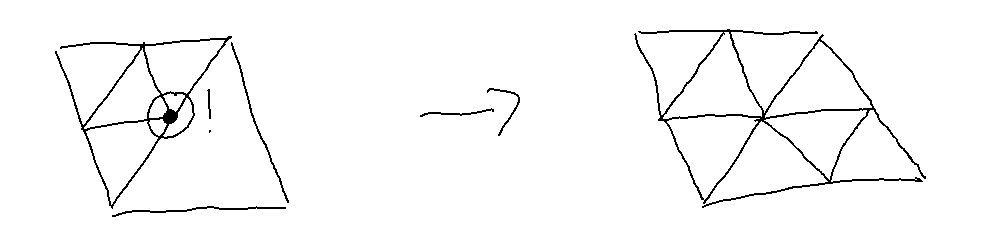
\includegraphics[width=\textwidth]{pics/Sketch10.png}
		\caption{Unnötig starke Verfeinerung um hängenden Knoten zu beheben}
		\label{AbbVerfeinerung}
	\end{center}
\end{figure}

Deshalb führen wir folgende Typen von Verfeinerungen ein:
\begin{itemize}
	\item \color{red}rote Verfeinerung\color{black}: normale Verfeinerung: Unterteile ein Dreick in 4 Teildreicke
	\item \color{green}grüne Verfeinerung\color{black}: verbinde den Mittelpunkt der \ul{längsten} Kante mit der entgegengesetzten Ecke
	\item \color{blue}blaue Verfeinerung\color{black}: Verbinde den Mittelpunkt der \underline{längsten} Kante mit der entgegengesetzten Ecke und mit einem Mittelpunkt einer anderen Kante
\end{itemize}

\begin{figure}[H]
	\center
	\begin{tikzpicture}[scale=1]
	\def \xone{0};
	\def \yone{0};
	\def \h{3};
	
	% first triangle   red
	\coordinate (A) at (\xone,\yone);
	\coordinate (B) at ($ (A) + (1.4*\h,0) $);
	\coordinate (C) at ($ (A) + (0.7*\h,0.7*\h) $);
	\coordinate (AB) at ($ (A) + (0.7*\h,0) $);
	\coordinate (AC) at ($ (A) + (0.35*\h,0.35*\h) $);
	\coordinate (BC) at ($ (A) + (1.05*\h,0.35*\h) $);

	%draw		
	\draw (A) -- (B) -- (C) --cycle;
	\draw[red] (AB) -- (AC) -- (BC) --cycle;
	\foreach \i in {A,B,C,AB,AC,BC}{
		\filldraw (\i) circle (1.5pt);
	}

	% second triangle   green
	\coordinate (A1) at (\xone + 1.6*\h,\yone);
	\coordinate (B1) at ($ (A1) + (1.4*\h,0) $);
	\coordinate (C1) at ($ (A1) + (0.7*\h,0.7*\h) $);
	\coordinate (AB1) at ($ (A1) + (0.7*\h,0) $);

	%draw			
	\draw (A1) -- (B1) -- (C1) --cycle;
	\draw[green] (AB1) -- (C1);
	\foreach \i in {A1,B1,C1,AB1}{
		\filldraw (\i) circle (1.5pt);
	}

	% third triangle   blue
	\coordinate (A2) at (\xone + 0.8*\h,\yone - \h);
	\coordinate (B2) at ($ (A2) + (1.4*\h,0) $);
	\coordinate (C2) at ($ (A2) + (0.7*\h,0.7*\h) $);
	\coordinate (AB2) at ($ (A2) + (0.7*\h,0) $);
	\coordinate (BC2) at ($ (A2) + (1.05*\h,0.35*\h) $);

	%draw			
	\draw (A2) -- (B2) -- (C2) --cycle;
	\draw[blue] (AB2) -- (C2);
	\draw[blue] (AB2) -- (BC2);
	\foreach \i in {A2,B2,C2,AB2}{
		\filldraw (\i) circle (1.5pt);
	}
\end{tikzpicture}
	\caption{Verfeinerung: rot,grün,blau}
	\label{AbbRefinement_types}
\end{figure}

\textbf{Schritt 4:}
\begin{enumerate}[label=\alph*)]
	\item $\eta_T\geq\gamma\cdot\eta_l\implies\text{ rote Verfeinerung}$
	\item drei hängende Knoten $\implies$ rote Verfeinerung
	\begin{figure}[!ht]
		\begin{center}
			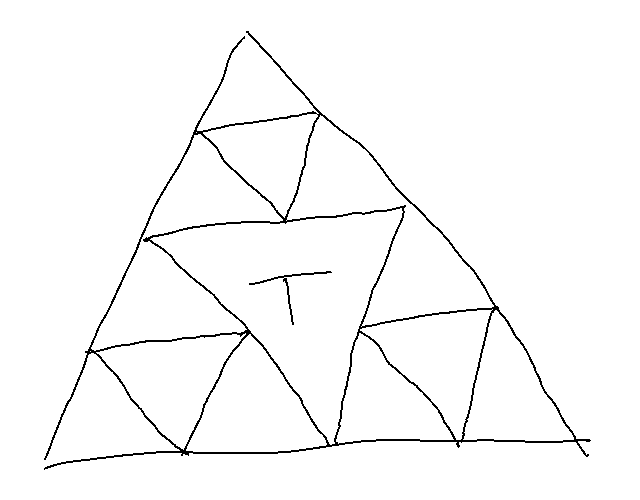
\includegraphics[width=0.4\textwidth]{pics/Sketch11.png}
			\caption{Fall b}
			\label{AbbVerfeinerungB}
		\end{center}
	\end{figure}
	\item zwei hängende Knoten, beide \underline{nicht} auf der längsten Kante $\implies$ rote Verfeinerung
	\begin{figure}[!ht]
		\begin{center}
			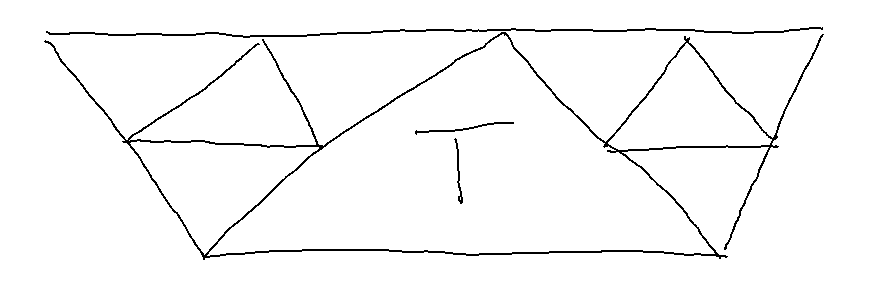
\includegraphics[width=0.4\textwidth]{pics/Sketch12.png}
			\caption{Fall c}
			\label{AbbVerfeinerungC}
		\end{center}
	\end{figure}
	\item zwei hängende Knoten, eine auf der längsten Kante $\implies$ blaue Verfeinerung
	\begin{figure}[!ht]
		\begin{center}
			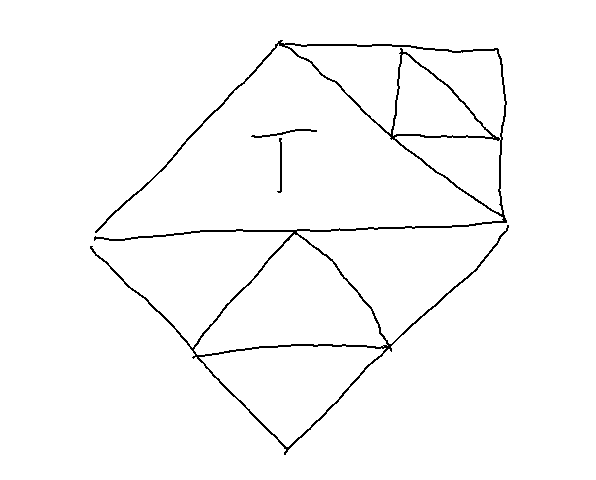
\includegraphics[width=0.4\textwidth]{pics/Sketch13.png}
			\caption{Fall d}
			\label{AbbVerfeinerungD}
		\end{center}
	\end{figure}
	\item ein hängender Knoten, \underline{nicht} auf der längsten Kante $\implies$ blaue Verfeinerung
	\begin{figure}[!ht]
		\begin{center}
			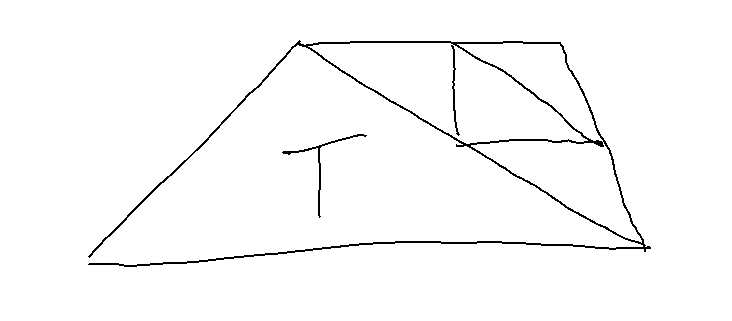
\includegraphics[width=0.4\textwidth]{pics/Sketch14.png}
			\caption{Fall e}
			\label{AbbVerfeinerungE}
		\end{center}
	\end{figure}
	\item ein hängender Knoten auf der längsten Kante $\implies$ grüne Verfeinerung
	\begin{figure}[!ht]
		\begin{center}
			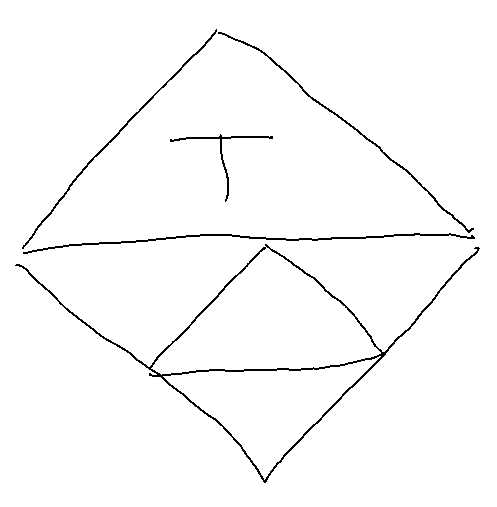
\includegraphics[width=0.3\textwidth]{pics/Sketch15.png}
			\caption{Fall f}
			\label{AbbVerfeinerungF}
		\end{center}
	\end{figure}
\end{enumerate}
	% This work is licensed under the Creative Commons
% Attribution-NonCommercial-ShareAlike 4.0 International License. To view a copy
% of this license, visit http://creativecommons.org/licenses/by-nc-sa/4.0/ or
% send a letter to Creative Commons, PO Box 1866, Mountain View, CA 94042, USA.
% vim: set noexpandtab:

\section{Stromlinien-Diffusions-Methode (SDFEM)} %7.
Hughes / Brooks 1979

\subsection{Motivation}
\begin{align*}
\left\lbrace
	\begin{array}{rl}
	-\varepsilon\cdot\Delta u+b\cdot \nabla u+c\cdot u=f&\text{ in }\Omega\\
	u=g&\text{ auf }\Gamma=\partial\Omega\\
	0<\varepsilon\ll 1&
	\end{array}
	\right.
\end{align*}

Für $\varepsilon=0$ ist dies eine PDE erster Ordnung, aber für $\varepsilon>0$ eine PDE zweiter Ordnung.
Beim Grenzübergang passieren "magische Dinge", die sich mit den bisher bekannten Verfahren nicht sinnvoll lösen lassen.
Es kommt zu Oszillationen.
Deshalb wurden die SDFEM-Verfahren erfunden.
Die Idee besteht darin aus das diskrete Problem noch $\delta_K$-mal das glatte Problem dazu zu addieren.\nl
\textbf{1D:}
\begin{align*}
	-\varepsilon\cdot u''+u'=0\text{ auf }(0,1),\qquad u(0)=0,\qquad u(1)=1
\end{align*}
\begin{figure}[!ht]
	\begin{center}
		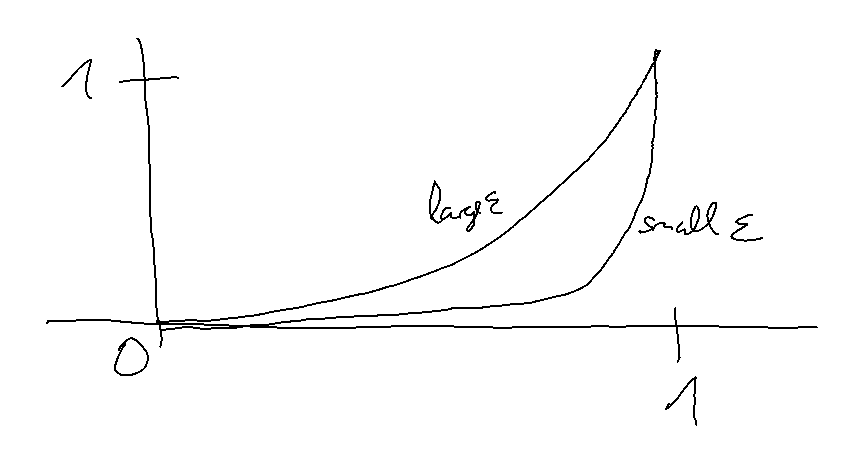
\includegraphics[width=0.7\textwidth]{pics/Sketch16.png}
		\caption{Skizze für kleines und großes $\epsilon$}
		\label{AbbEinfachesStromlinienProblem}
	\end{center}
\end{figure}

ersetze $\varepsilon$ durch Gitterparameter $h$.\\
$\implies$ keine Oszillation, aber "Verschmierung" %smearing

Verschmierung hauptsächlich in Seitenwindrichtung
$b$ und $b^\perp$ sind orthogonale Einheitsvektoren
\begin{align*}
	\Delta u&=\frac{\partial^2 u}{\partial x^2}+\frac{\partial^2 u}{\partial y^2}
	=\frac{\partial^2 u}{\partial b^2}+\frac{\partial^2 u}{\partial (b^T)^2}\\
	\varepsilon\cdot\Delta u&\to\varepsilon\cdot\frac{\partial^2 u}{\partial(b^T)^2}+h\cdot\frac{\partial^2 u}{\partial b^2}
\end{align*}
Hier nur Konvergenz erster Ordnung in $h$.

\subsection{SDFEM Diskretisierung}
\textbf{Modellproblem}
\begin{align}\label{eq7.2_1}\tag{1}
	\left\lbrace\begin{array}{rl}
		-\varepsilon\Delta u+b\cdot\nabla u+cu&=f\text{ in }\Omega\\
		u&=0\text{ auf }\Gamma=\partial\Omega
	\end{array}\right.
\end{align}
Diskretisierung: stetige $P_r$-Elemente $\to V_h\subseteq H_0^1(\Omega)$\\
$u\in H^2(\Omega)$, $b,c$ hinreichend glatt
\begin{align}\nonumber
	-\varepsilon\Delta u+b\cdot \nabla u+cu&= f&&\text{ im }L^2\text{- Sinn}\\
	\implies\Big(-\varepsilon\Delta u+b\cdot\nabla u+cu,b\cdot\nabla v_h\Big)_K&=\big(f,b\cdot\nabla v_h\big)_K
	&&\forall K\in\T_h,v_h\in V_h
	\label{eq7.2_2}\tag{2}
\end{align}

mit
\begin{align*}
	(\varphi,\psi):&=\int\limits_K\varphi(x)\cdot\psi(x)\d x
\end{align*}
Zusätzlich: (Einschränkung auf schwache Formulierung von $V_h$):
\begin{align*}\label{eq7.2_3}\tag{3}
	\varepsilon(\nabla u,\nabla v)+(b\cdot\nabla u+ cu,v_h)=(f,v_h)\qquad\forall v_h\in V_h
\end{align*}
$(\cdot,\cdot)=(\cdot,\cdot)_\Omega$\nl
$u$ erfüllt:
\begin{align}\label{eq7.2_4}\tag{4}
	a_h(u,v_h)&=f_h(v_h)\qquad\forall v_h\in V_h
\end{align}
wobei
\begin{align}\label{eq7.2_5}\tag{5}
	a_h(u,v)&:=\varepsilon(\nabla u,\nabla v)+(b\cdot\nabla u+cu, v)\\\nonumber
	&\qquad+\sum\limits_{K\in\T_h}\delta_K\Big(-\varepsilon\Delta u+b\cdot\nabla u+cu,b\cdot\nabla v\Big)_K\\
	\label{eq7.2_6}\tag{6}
	f_h(v_h)&:=(f,v_h)+\sum\limits_{K\in\T_h}\delta_K(f,b\cdot\nabla v)_K
\end{align}

\textbf{Idee:} Diskretes Problem:\\
Finde $u_h\in V_h$ so, dass
\begin{align}\label{eq7.2_7}\tag{7}
	a_h(u_h,v_h)&=f_h(v_h)\qquad\forall v_h\in V_h
\end{align}
Damit folgt aus \eqref{eq7.2_4} und \eqref{eq7.2_7}:
\begin{align}\label{eq7.2_8}\tag{8}
	a_h(u-u_h,v_h)=0\qquad\forall v_h\in V_h
\end{align}
Also die Galerkin Orthogonalität.\nl
\textbf{Wahl von $\delta_k$:}\\
Die \textbf{lokale Peclét-Zahl} ist
\begin{align*}
	p_{e_K}:=\frac{\Vert b\Vert_{0,\infty,K}}{2\cdot\varepsilon}\cdot h_K
\end{align*}
Hängt mit der Beziehung zwischen Konvention und Diffusion zusammen.
\begin{align}\label{eq7.2_9}\tag{9}
	\delta_K:=\left\lbrace\begin{array}{cl}
		\delta_0 h_K, &\falls p_{e_K}>1\\
		\frac{\delta_1 h_K^2}{\varepsilon}, &\falls p_{e_K}\leq 1
	\end{array}\right.
\end{align}
Hierbei sind $\delta_0,\delta_1$ Konstanten.\nl
\textbf{Spezialfall: 2D, stetige $P_1$-Elemente, $c\equiv0$, $b\equiv(b_1,b_2)=$ konstant}\\
Also erhält man
\begin{align*}
	a_h(u_h,v_h)&=\varepsilon\big(\nabla u_h,\nabla v_h\big)+(b\cdot\nabla u_h,v_h)
	+\underbrace{\sum\limits_{K\in\T_h}\delta_K\big(b\cdot\nabla u_h,b\cdot\nabla v_h\big)_K}_{\text{zusätzliche Diffsion in Richtung }b}
\end{align*}

\subsection{Konvergenzanalysis}
Annahmen:
\begin{itemize}
	\item $b,c,f$ seien hinreichend glatt
	\item für die eindeutige Lösbarkeit nehmen wir an
	\begin{align}\label{eq7.3_10}\tag{10}
		c-\frac{1}{2}\div(b)\geq0\text{ in }\Omega
	\end{align}
	\item $V_h$: stetige $P_r$-Elemente, $V_h\subseteq H_0^1(\Omega)$
	\item Lokalinversen-Ungleichung
	\begin{align}\label{eq7.3_11}\tag{11}
		\Vert\Delta v_h\Vert_{0,2,K}\leq\mu_{\text{inv}}\cdot h^{-1}_K\cdot|v_h|_{1,2,K}
		\qquad\forall v_h\in V_h,\forall K\in\T_h
	\end{align}
	$\mu_{\text{inv}}$ ist unabhängig von $K$
	\item SD-Norm
	\begin{align}\label{eq7.3_12}\tag{12}
		\Vert v\Vert_{\text{SD}}:=\left(\varepsilon|v|_{1,2,\Omega}^2+c_0\Vert v\Vert_{0,2,\Omega}^2+\sum\limits_{K\in\T_h}\delta_K\Vert b\cdot\nabla v\Vert^2_{0,2,K}\right)^{\frac{1}{2}}
	\end{align}
\end{itemize}

\begin{lemma}[Koerzivität]\label{lemma7.1Koerzivitaet}
	Sei
	\begin{align*}
		c_k:=\Vert c\Vert_{0,\infty,\Omega}=\max\limits_{x\in K}\big|c(x)\big|>0
	\end{align*}
	und
	\begin{align}\label{eq7.3_13}\tag{13}
		0<\delta_K\leq\frac{1}{2}\cdot\min\left\lbrace\frac{c_0}{c_K^2},\frac{h_K^2}{\varepsilon\cdot\mu_{\text{inv}}^2}\right\rbrace
	\end{align}
	Dann ist $a_h$ koerziv im folgenden Sinn:
	\begin{align}\label{eq7.3_14}\tag{14}
		a_h(v_h,v_h)\geq\frac{1}{2}\cdot\Vert v_h\Vert_{\text{SD}}^2\qquad\forall v_h\in V_h
	\end{align}
\end{lemma}

\begin{proof}
	Erinnerung:
	\begin{align*}
		\big(b\cdot\nabla v_h,v_h\big)&=\frac{1}{2}\cdot\big(\div(b)\cdot v_h^2\big)
	\end{align*}
	Damit also:
	\begin{align*}
		\implies a_h(v_h,v_h)
		&=\varepsilon(\nabla v_h,\nabla v_h)+(b\cdot\nabla v_h,v_h)+(c \cdot v_h,v_h)\\
		&~+\sum\limits_{K\in\T_h}\delta_K\Big(-\varepsilon\Delta v_h+b\cdot\nabla v_h+c \cdot v_h,b\cdot\nabla v_h\Big)_K\\
		&=\varepsilon|v_h|^2_{1,2,\Omega}+\Big(\underbrace{c-\frac{1}{2}\cdot\div(b)}_{\geq c_0>0},v_h^2\Big)+\sum\limits_{K\in\T_h}\delta_K\big(b\cdot\nabla v_h,b\cdot \nabla v_h\big)_K\\
		&~+\underbrace{\sum\limits_{K\in\T_h}\delta_K\big(-\varepsilon\Delta v_h,b\cdot\nabla v_h\big)_K}_{=:T_1}
		+\underbrace{\sum\limits_{K\in\T_h}\delta_K\big(c \cdot v_h,b\cdot\nabla v_h\big)_K}_{=:T_2}\\
		&\geq\underbrace{\varepsilon|v_h|^2_{1,2,\Omega}+c_0\Vert v_h\Vert^2_{0,2,\Omega}+\sum\limits_{K\in\T_h}\delta_K\Vert b\cdot\nabla v_h\Vert^2_{0,2,K}}_{=\Vert v\Vert^2_{\text{SD}}}-|T_1|-|T_2|
	\end{align*}
	Jetzt müssen wir noch $T_1$ und $T_2$ abschätzen.
	\begin{align*}
		|T_1|
		&\leq\sum\limits_{K\in\T_h}\delta_K\varepsilon\Big|(\Delta v_h,b\cdot\nabla v_h)_K\Big| \\
		&\overset{\text{CS}}{\leq}
		\sum\limits_{K\in\T_h}\delta_K\varepsilon\Vert\Delta v_h\Vert_{0,2,K}\cdot\Vert b\cdot\nabla v_h\Vert_{0,2,K}\\
	\end{align*}
	Mit
	\begin{align*}
		\alpha\beta
		&\leq\alpha^2+\frac{1}{4}\beta^2\\
		\alpha&=\varepsilon\delta_K^{\frac{1}{2}}\Vert\Delta v_h\Vert_{0,2,K}\\
		\beta&=\delta_K^{\frac{1}{2}}\Vert b\cdot\nabla v_h\Vert_{0,2,K}
	\end{align*}
	gilt
	\begin{align*}
		&\sum\limits_{K\in\T_h}\delta_K\varepsilon\Vert\Delta v_h\Vert_{0,2,K}\cdot\Vert b\cdot\nabla v_h\Vert_{0,2,K} \\
		&\leq
		\sum\limits_{K\in\T_h}\underbrace{\varepsilon^2\delta_K\underbrace{\Vert\Delta v_h\Vert^2_{0,2,K}}_{\overset{\eqref{eq7.3_11}}{\leq}\mu^2_{\text{inv}} h_K^{-1}|v_h|^2_{1,2,K}}}_{\leq\underbrace{\varepsilon^2\delta_K\mu^2_{\text{inv}} h_K^{-2}}_{\overset{\eqref{eq7.3_13}}{\leq}\frac{\varepsilon}{2}}|v_h|^2_{1,2,K}}\\
		&\leq\frac{1}{2}\varepsilon|v_h|^2_{1,2,\Omega}+\frac{1}{4}\sum\limits_{K\in\T_h}\delta_K\Vert b\cdot\nabla v_h\Vert^2_{0,2,K}
	\end{align*}
	Für $T_2$ erhalten wir die Abschätzung
	\begin{align*}
		|T_2|
		&\leq\sum\limits_{K\in\T_h}\delta_K\Big|(c \cdot v_h,b\cdot\nabla v_h)_K\Big|\\
		&\leq\sum\limits_{K\in\T_h}\delta_K c_K\Vert v_h\Vert_{0,2,K}\Vert b\cdot\nabla v_h\Vert_{0,2,K}
	\end{align*}
	Mit
	\begin{align*}
		\alpha&=\delta_K^{\frac{1}{2}}c_K\Vert v_h\Vert_{0,2,K}\\
		\beta&=\delta_K^{\frac{1}{2}}\Vert b\cdot\nabla v_h\Vert_{0,2,K}
	\end{align*}
	gilt
	\begin{align*}
		&\sum\limits_{K\in\T_h}\delta_K c_K\Vert v_h\Vert_{0,2,K}\Vert b\cdot\nabla v_h\Vert_{0,2,K} \\
		&\leq\sum\limits_{K\in\T_h}\underbrace{\delta_K c_K^2}_{\overset{\eqref{eq7.3_13}}{\leq}\frac{c_0}{2}}\Vert v_h\Vert^2_{0,2,K}+\frac{1}{4}\sum\limits_{K\in\T_h}\delta_K\Vert b\cdot\nabla v_h\Vert^2_{0,2,K}\\
		&\leq\frac{1}{2}c_0\Vert v_h\Vert^2_{0,2,\Omega}+\frac{1}{4}\sum\limits_{K\in\T_h}\delta_K\Vert b\cdot\nabla v_h\Vert^2_{0,2,K}
	\end{align*}
	Folglich gilt insgesamt

	\begin{align*}
		a_h(v_h,v_h)
		&\geq\Vert v_h\Vert^2_{\text{SD}}-|T_1| -|T_2| \\
		&\geq\Vert v_h\Vert^2_{\text{SD}}\underbrace{
			\begin{array}{l}
				-\frac{1}{2}\varepsilon\vert v_h\vert_{1,2,\Omega}
			-\frac{1}{4}\sum\limits_{K\in\T_h}\delta_K\Vert b\cdot\nabla v_h\Vert^2_{0,2,K}\\
			-\frac{1}{2}c_0\Vert v_h\Vert_{0,2,\Omega}
			-\frac{1}{4}\sum\limits_{K\in\T_h}\delta_K\Vert b\cdot\nabla v_h\Vert^2_{0,2,K}
			\end{array}
			}_{=-\frac{1}{2}\Vert v_h\Vert_{\text{SD}}^2}\\
		&=\frac{1}{2}\Vert v_h\Vert^2_{\text{SD}}
	\end{align*}
\end{proof}

\begin{bemerkung}\
	\begin{itemize}
		\item $P_1$-Elemente: \eqref{eq7.3_13} kann ersetzt werden durch
		\begin{align*}
			0<\delta_K\leq\frac{1}{2}\frac{c_0}{c_K^2}\qquad\forall K\in\T_h
		\end{align*}
		\item Die Bedingung $\delta_K\leq\frac{1}{2}\frac{c_0}{c_K^2}$ kann ersetzt werden durch $\delta_K c_K^2\leq\frac{1}{2}c_0$. Dies erlaubt $c_K=0$.
		\item Eine geeignete Wahl von $\delta_0, \delta_1$ (klein genug) in \eqref{eq7.2_9} erhält die Gültigkeit von \eqref{eq7.3_13}
	\end{itemize}
\end{bemerkung}

\begin{align*}
	\frac{1}{2}\Vert u_h\Vert^2_{\text{SD}}
	&\leq a_h(u_h,u_h)\\
	&=f_h(u_h)\\
	&=f(u_h)+\sum\limits_{K\in\T_h}\delta_K(f,b\cdot\nabla u_h)_K\\
	\overset{\text{CS}}&{\leq}
	\Vert f\Vert_{0,2,\Omega}\frac{1}{c_0}\sqrt{c_0}\Vert u_h\Vert_{0,2,\Omega}+\sum\limits_{K\in\T_h}\delta_K^{\frac{1}{2}}\Vert f\Vert_{0,2,K}\delta_K^{\frac{1}{2}}\Vert b\cdot\nabla u_h\Vert_{0,2,K}\\
	&\leq\frac{1}{\sqrt{c_0}}\Vert f\Vert_{0,2,\Omega}\Vert u_h\Vert_{\text{SD}}+\left(\sum\limits_{K\in\T_h}\delta_K\Vert f\Vert^2_{0,2,K}\right)^{\frac{1}{2}}\Vert u_h\Vert_{\text{SD}}\\
\end{align*}
Teilen durch $\frac{\Vert u_h \Vert_{SD}}{2}$ auf beiden Seiten ergibt
\begin{align*}
	\Vert u_h\Vert_{\text{SD}} \leq C(f)
\end{align*}

Wir habe zusätzliche Kontrolle über die Ableitungen in Streamline-Richtung
\begin{align*}
	\left(\sum\limits_{K\in\T_h}\delta_K\Vert b\cdot\nabla u_h\Vert^2_{0,2,K}\right)^{\frac{1}{2}} \leq C(f)
\end{align*}
wobei $\delta_K \sim h_K \text{, wenn } p_{e_K} > 1$.

\begin{theorem}\label{theorem7.2}
	Sei $\delta_k$ gemäß \eqref{eq7.2_9} und \eqref{eq7.3_13} gewählt.
	Wenn wir stetige $P_r$-Elemente nutzen, dann gilt
	\begin{align*}
		\Vert u-u_h\Vert_{\text{SD}}&\leq C\cdot\left(\varepsilon^{\frac{1}{2}}+h^{\frac{1}{2}}\right)\cdot h^r\cdot |u|_{r+1,2,\Omega}\mit\\
		\Vert v\Vert_{\text{SD}}^2\overset{\text{Def}}&=\varepsilon\cdot|v|^2_{1,2,\Omega}+c_0\Vert v\Vert^2_{0,2,\Omega}+\sum\limits_{K\in\T_h}\delta_K\Vert b\cdot\nabla v\Vert^2_{0,2,K}
	\end{align*}
\end{theorem}

\begin{proof}
	Sei $I_h u\in V_h$ die Interpolierende der exakten Lösung $u$. Setze
	\begin{align*}
		w_h:=I_h u-u_h\in V_h.
	\end{align*}
	Dann folgt aus Lemma \ref{lemma7.1Koerzivitaet}:
	\begin{align*}
		\frac{1}{2}\Vert w_h\Vert^2_{\text{SD}}
		&\leq a_h(w_h,w_h)
		=a_h(I_h u-u, w_h)+\underbrace{a_h(u-u_h,w_h)}_{=0}
	\end{align*}
	Abschätzung für $a_h$ termweise:
	\begin{align*}
		\Big|\varepsilon\big(\nabla(I_h u-u),\nabla w_h\big)\Big|
		\overset{\text{CS}}&\leq
		\varepsilon^{\frac{1}{2}}\underbrace{|I_h u-u|_{1,2,\Omega}}_{\leq C h^r|u|_{r+1,2,\Omega}}\underbrace{\varepsilon^{\frac{1}{2}}|w_h|_{1,2,\Omega}}_{\leq\Vert w_h\Vert_{\text{SD}}}\\
		&\leq C\varepsilon^{\frac{1}{2}} h^r|u|_{r+1,2,\Omega}\Vert w_h\Vert_{\text{SD}}
	\end{align*}
	Die Idee
	\begin{align*}
		\Big|\big(b\cdot\nabla(I_h u-u),w_h\big)\Big|
		&\leq
		\big\Vert b\cdot\nabla(I_h u-u)\big\Vert_{0,2,\Omega}\Vert w_h\Vert_{0,2,\Omega}\\
		&\leq\frac{C}{\sqrt{c_0}}h^r|u|_{r+1,2,\Omega}\Vert w_h\Vert_{\text{SD}}
	\end{align*}
	ist \underline{nicht} optimal!
	Stattdessen probieren wir partielle Integration:
	\begin{align*}
		\big(b\cdot\nabla(I_h u-u),w_h\big)
		&=-\big(b\cdot\nabla w_h,I_h u-u\big)-\big(\div(b)w_h,I_h u-u\big)\\
		%\implies
		\Big|\big(b\cdot\nabla(I_h u-u)+c (I_h u-u),w_h\big)\Big|
		&\leq\Big|\big((c-\div(b))(I_h u-u),w_h\big)\Big|+\Big|\big(I_h u-u,b\cdot\nabla w_h\big)\Big|\\
		\implies
		\Big|\big((c-\div(b))(I_h u-u),w_h\big)\Big|
		\overset{\text{CS}}&\leq
		\underbrace{\big\Vert c-\div(b)\big\Vert_{0,\infty,\Omega}}_{\leq C}\underbrace{\Vert I_h u-u\Vert_{0,2,\Omega}}_{\leq C h^{r+1}|u|_{r+1,2,\Omega}}\underbrace{\Vert w_h\Vert_{0,2,\Omega}}_{\leq\frac{1}{\sqrt{c_0}}\Vert w_h\Vert_{\text{SD}}}\\
		&\leq\frac{C}{\sqrt{c_0}}h^{r+1}|u|_{r+1,2,\Omega}\Vert w_h\Vert_{\text{SD}}
	\end{align*}
	Zum Schluss noch
	\begin{align*}
		\Big|\big(I_h u-u,b\cdot\nabla w_h\big)\Big|
		\overset{\text{CS}}&\leq
		\sum\limits_{K\in\T_h}\Vert I_h u-u\Vert_{0,2,K}\Vert b\cdot\nabla w_h\Vert_{0,2,K}\\
		&=\sum\limits_{K\in\T_h}\delta_K^{-\frac{1}{2}}\underbrace{\Vert I_h u-u\Vert_{0,2,K}}_{\leq C h^{r+1}_K|u|_{r+1,2,K}}\delta_K^{\frac{1}{2}}\Vert b\cdot\nabla w_h\Vert_{0,2,K}\\
		&\leq C\underbrace{\left(\sum\limits_{K\in\T_h}\delta_K^{-1} h_K^{2r+2}|u|^2_{r+1,2,K}\right)^{\frac{1}{2}}}_{
			\leq h^r\left(\sum\limits_{K\in\T_h}\delta_K^{-1} h_K^2|u|^2_{r+1,2,K}\right)^{\frac{1}{2}}
		}\Vert w_h\Vert_{\text{SD}}
	\end{align*}
	Setzen wir dies alles zusammen, so erhalten wir
	\begin{align*}
		&\left|\sum\limits_{K\in\T_h}\delta_K\Big(-\varepsilon\Delta(I_h u-u)+b\cdot\nabla(I_h u-u)+c(I_h u-u),b\cdot\nabla w_h\Big)_K\right|\\
		&\leq\sum\limits_{K\in\T_h}\delta_K^{\frac{1}{2}}\Big(\varepsilon\underbrace{\Vert\Delta(I_h u-u)\Vert_{0,2,K}}_{\leq C h^{r-1}|u|_{r+1,2,K}}+\Vert b\Vert_{0,\infty,K}\underbrace{|I_h u-u|_{1,2,K}}_{\leq C h^r|u|_{r+1,2,K}}+\Vert c\Vert_{0,\infty,K}\underbrace{\Vert I_h u-u\Vert_{0,2,K}}_{\leq C h^{r+1}|u|_{r+1,2,K}}\Big)\\
		&\qquad\cdot\delta_K^{\frac{1}{2}}\Vert b\cdot\nabla w_h\Vert_{0,2,K}\\
		&\leq C h^r\left(\sum\limits_{K\in\T_h}\Big(\delta_k\varepsilon^2 h^{-2}_K+\delta_K+\delta_K h^2_K\Big)|u|^2_{r+1,2,K}\right)^{\frac{1}{2}}\Vert w_h\Vert_{\text{SD}}
	\end{align*}
	Kurzer Einschub/Zwischenrechnung:
	\begin{align*}
		&\delta_K^{-1} h_K=\left\lbrace\begin{array}{cl}
			\frac{h^2_K}{\delta_0 h_K}=\frac{1}{\delta_0}h_K, & \falls p_{e_k}>1\\
			\frac{h_K}{\frac{\delta_1 h_K^2}{\varepsilon}}=\frac{\varepsilon}{\delta_1}, &\falls p_{e_k}\leq1
		\end{array}\right.
		\leq C(\varepsilon+h)\\
		&\delta_K\varepsilon^2 h_K^{-2}+\delta_K+\delta_K\underbrace{h_K^2}_{\leq1}
		\leq\underbrace{\delta_K\varepsilon^2 h_K^{-2}}_{
			\overset{\eqref{eq7.3_13}}{\leq}\varepsilon^2 h_K^{-2}\frac{1}{2}\frac{h_K^2}{\varepsilon \mu^2_{\text{inv}}}\leq C\varepsilon
		}+\delta_K
	\end{align*}
	Fall $p_{e_k}>1$: $\delta_k=\delta_0 h_K$\nl
	Fall $p_{e_k}\leq1$:
	\begin{align*}
		p_{e_k}\leq1\Longleftrightarrow\frac{\Vert b\Vert_{0,\infty,K}}{2\varepsilon}h_K&\leq 1\\
		h_K&\leq C\varepsilon\\
		\delta_K=\delta_1\frac{h_K^2}{\varepsilon}&\leq C\varepsilon
	\end{align*}
	Die Abschätzung funktioniert also immer. Nutzen wir sie, so erhalten wir:
	\begin{align*}
		\frac{1}{2}\Vert w_h\Vert^2_{\text{SD}}&\leq C h^r\left(\varepsilon^{\frac{1}{2}}+h^{\frac{1}{2}}\right)|u|_{r+1,2,\Omega}\Vert w_h\Vert_{\text{SD}}\\
		\Vert w_h\Vert_{\text{SD}}&\leq C h^r\left(\varepsilon^{\frac{1}{2}}+h^{\frac{1}{2}}\right)|u|_{r+1,2,\Omega}
	\end{align*}
	Damit können wir die eigentliche Abschätzung beginnen
	\begin{align*}
		\Vert u-u_h\Vert_{\text{SD}}
		&\leq\Vert u-I_h u\Vert_{\text{SD}}+\Vert\underbrace{I_h u-u_h}_{=w_h}\Vert_{\text{SD}}
		\leq Ch^r\left(\varepsilon^{\frac{1}{2}}+h^{\frac{1}{2}}\right)|u|_{r+1,2,\Omega}\\
		\Vert u-I_h u\Vert^2_{\text{SD}}
		&=\varepsilon|I_h u-u|^2_{1,2,\Omega}+c_0\Vert I_h u-u\Vert^2_{0,2,\Omega}+\sum\limits_{K\in\T_h}\delta_K\Vert b\cdot\nabla(I_h u-u)\Vert^2_{0,2,K}\\
		&\leq C\varepsilon h^{2r}|u|^2_{r+1,2,\Omega}+C h^{2r+2}|u|^2_{r+1,2,\Omega}+C h^{2r+2}|u|^2_{r+1,2,\Omega}\\
		&~+Ch^{2r}\sum\limits_{K\in\T_h}\underbrace{\delta_K}_{\leq C(\varepsilon+h)}|u|^2_{r+1,2,K}\\
		&\leq C(\varepsilon+h) h^{2r}|u|^2_{r+1,2,\Omega}
	\end{align*}
\end{proof}

\begin{align*}
	&\varepsilon<<h\implies \delta_K\approx h_K\\
	\implies&\Vert u-u_h\Vert_{\text{SD}}\leq C\cdot h^{r+\frac{1}{2}}\cdot|u|_{r+1,2,\Omega}\\
	\implies& \Vert u-u_h\Vert_{0,2,\Omega}\leq C\cdot h^{r+\frac{1}{2}}\cdot|u|_{r+1,2,\Omega}\\
	&\Bigg(\sum\limits_{K\in\T_h}\approx h_K\big\Vert b\cdot\nabla(u+h_K)\big\Vert_{0,2,K}\Bigg)^{\frac{1}{2}}
	\leq C\cdot h^{r+\frac{1}{2}}\cdot|u|_{r+1,2,\Omega}\\
	\implies&\text{nicht-optimal hinsichtlich Interpolationsfehler}\\
	\implies& \big\Vert b\cdot\nabla(u-u_h)\big\Vert_{0,2,\Omega}\leq C\cdot h^r\cdot|u|_{r+1,2,\Omega}\\
	\implies&\text{optimale Konvergenz in Streamline-Richtung}
\end{align*}
	% This work is licensed under the Creative Commons
% Attribution-NonCommercial-ShareAlike 4.0 International License. To view a copy
% of this license, visit http://creativecommons.org/licenses/by-nc-sa/4.0/ or
% send a letter to Creative Commons, PO Box 1866, Mountain View, CA 94042, USA.

\section{Argmin-Theoreme in \texorpdfstring{$C(\R)$}{C(R)}} %8
Erinnere an folgende Probleme, vergleiche  1.2 und 1.5 (Median)\\ %TODO
Wann überträgt sich die Konvergenz (f.s. oder in Verteilung) von stetigen stochastischen Prozessen auf deren Minimalstellen?

\begin{definition}\label{definition8.1}
	Sei $f\in C(\R)$.
	\begin{enumerate}[label=(\arabic*)]
		\item $\begin{aligned}
			A(f)=\argmin(f):=\left\lbrace t\in\R:f(t)=\inf\limits_{s\in\R} f(s)\right\rbrace
		\end{aligned}$ = Menge aller Minimalstellen
		\item $\tau\in A(f)$ heißt \textbf{wohl-separiert} 
		\begin{align*}
			:\Longleftrightarrow\inf\Big\lbrace f(t):|t-\tau|\geq\varepsilon\Big\rbrace>f(\tau)\qquad\forall 0<\varepsilon\in\Q
		\end{align*}
	\end{enumerate}
\end{definition}

\begin{bemerkungnr}\label{bemerkung8.2}\
	\begin{enumerate}[label=(\arabic*)]
		\item $A(f)\neq\emptyset$ ist natürlich nicht ausgeschlossen, aber in jedem Fall ist $A(f)$\\ \underline{abgeschlossen} in $\R$, denn:\\
		Sei $(t_n)_{n\in\N}\subseteq A(f)$ mit $t_n\stackrel{n\to\infty}{\longrightarrow}t.$ Dann gilt:
		\begin{align*}
			f(t)&=\limn\underbrace{f(t_n)}_{=\inf\limits_{s\in\R}f(s)}=\inf\limits_{s\in\R}f(s)
			\implies t\in A(f)
		\end{align*}
		\item $\tau$ wohl-separariert $\implies\tau$ eindeutig, denn:\\
		Sei $\tilde{\tau}\in A(f)$ und $\tilde{\tau}\neq\tau$. Also:
		\begin{align}\label{eqBemerkung8.2Stern}\tag{$\ast$}
			\exists 0&<\varepsilon\in\Q:\big|\tau-\tau|>\varepsilon\\\nonumber
			\inf\limits_{s\in\R}f(s)
			\overset{\tilde{\tau}\in A(f)}&=
			f(\tau)
			\overset{\eqref{eqBemerkung8.2Stern}}{\geq}
			\inf\Big\lbrace f(t):|t-\tau|\geq\varepsilon\Big\rbrace
			\overset{\tau\text{ wohl-sep}}{\geq}
			f(\tau)
			\overset{\tau\in A(f)}{=}
			\inf\limits_{s\in\R} f(s)
		\end{align}
		Dies ist ein Widerspruch!
	\end{enumerate}
\end{bemerkungnr}

\begin{beisp}
	Wann ist eine Minimalstelle eindeutig, aber nicht wohlsepariert?
	\begin{figure}[H]
		\begin{center}
			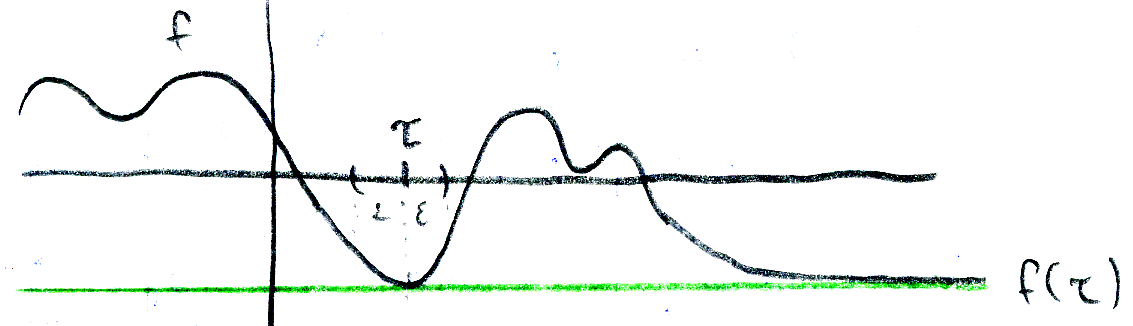
\includegraphics[width=1\textwidth]{./pics/MSTAT003.png}
			\caption{$\tau$ eindeutig, aber Infimum von $(\tau-\varepsilon,\tau+\varepsilon)$ ist auch $f(\tau)$!}
			\label{AbbMinimalstelleEindeutigNichtWohlsepariert}
		\end{center}
	\end{figure}
\end{beisp}

\begin{satz}\label{satz8.3}
	Seien $f,f_n,n\in\N$ aus $C(\R)$, $\tau_n\in A(f_n)\neq\emptyset~\forall n\geq N_0\in\N$ 
	(also $\tau_n$ ist eine Minimalstelle, ab einem gewissen Zeitpunkt $N_0$.)
	und $\tau\in A(f)$ sei wohl-separiert.
	Falls
	\begin{align}\label{eqSatz8.3_1}\tag{1}
		\big\Vert f_n-f\big\Vert\overset{\text{Def}}{=}\sup\limits_{t\in\R}\big|f_n(t)-f(t)\big|\overset{n\to\infty}{\longrightarrow}0
	\end{align}
	so folgt
	\begin{align*}
		\tau_n\overset{n\to\infty}{\longrightarrow}\tau
	\end{align*}
\end{satz}

\begin{proof}
	Sei $0<\varepsilon\overset{\text{oBdA}}{\in}\Q$. Es folgt:
	\begin{align*}
		s(\varepsilon)&:=\inf\limits\big\lbrace f(t):|t-\tau|\geq\varepsilon\big\rbrace
		\overset{\text{Def wohl-sep}}{>}
		f(\tau)\\
		\implies
		\delta&:=\delta(\varepsilon):=\frac{1}{3}\cdot\big(s(\varepsilon)-f(\tau)\big)>0\\
		\overset{\eqref{eqSatz8.3_1}}{\implies}
		\exists n_0&=n_0(\delta)\in\N:\forall n\geq n_0:
		\Vert f_n-f\Vert\leq\delta
	\end{align*}
	Für alle $n\geq\max\limits(N_0,n_0)$ gilt:\\
	Falls $t\in\R$ mit $|t-\tau|\geq\varepsilon$, so folgt:
	\begin{align*}
		f_n(t)-f_n(\tau)
		&=\underbrace{f_n(t)-f(t)}_{\geq\underbrace{-\underbrace{\Vert f_n-f\Vert}_{\leq\delta}}_{\geq-\delta}}+\underbrace{\underbrace{f(t)}_{\geq s(\varepsilon)}-f(\tau)}_{\geq s(\varepsilon)-f(\tau)=3\delta}+\underbrace{f(\tau)-f_n(\tau)}_{\geq-\delta}\\
		&\geq-\delta+3\cdot\delta-\delta\\
		&=\delta>0
	\end{align*}
	Es folgt
	\begin{align}\label{eqProofSatz8.3Stern}\tag{$\ast$}
		f_n(t)>f_n(\tau)\qquad\forall t\in\R\mit|t-\tau|\geq\varepsilon
	\end{align}
	Folglich gilt $|\tau_n-\tau|<\varepsilon$, denn sonst folgte aus \eqref{eqProofSatz8.3Stern}, dass
	$f_n(\tau_n)>f_n(\tau)$ im Widerspruch zu $\tau_n$ ist Minimalstelle von $f_n$.\\
	Somit gezeigt:
	\begin{align*}
		\forall\varepsilon\in\Q\cap(0,\infty):\exists m_0=m_0(\varepsilon):=\max\limits(N_0,n_0):\forall n\geq m_0:|t_n-\tau|<\varepsilon
	\end{align*}
\end{proof}

Satz \ref{satz8.3} lässt sich problemlos von $\R$ auf offene Intervalle $I=(a,b)$ übertragen.\nl
Für kompakte Intervalle $I=[a,b]$, $a<b\in\R$ muss $\tau$ nur eindeutig sein.
Es gilt:

\begin{satz}\label{satz8.4}
	Sei also $I=[a,b]$ kompaktes Intervall und seien $f,f_n,n\in\N$ aus $C(I)$. 
	Dann gilt:
	\begin{enumerate}[label=(\arabic*)]
		\item $\begin{aligned}
			A(f_n)\neq\emptyset\qquad\forall n\in\N
		\end{aligned}$
		\item Falls $\tau$ \underline{eindeutige} Minimalstelle von $f$ ist und falls
		\begin{align*}
			\Vert f_n-f\Vert_I:=\sup\limits_{t\in I}\big|f_n(t)-f(t)\big|\overset{n\to\infty}{\longrightarrow}0
		\end{align*}
		so gilt für \underline{jede} Auswahl $\tau_n\in A(f)$:
		$\tau_n\overset{n\to\infty}{\longrightarrow}\tau$
	\end{enumerate}
\end{satz}

%Ferger: "In irgendeinem der Seminarräumen ist mal eine Tafel von der Wand gefallen. Und ich möchte jetzt nicht unter so einer Tafel begraben liegen.
% Vielleicht ist das für einen Professor ein schöner Tod. Aber bitte jetzt noch nicht."
% "Ich bin ja von Natur aus etwas ängstlich. Es gab da mal so ein lustiges Lied und da singt der Sänger: "Leute seid nicht feige, lasst mich ...""

\begin{proof}
	\underline{Zeige (1):}\\
	Folgt, da jede stetige Funktion auf einem Kompaktum das Infimum annimmt.\nl
	\underline{Zeige (2):}\\
	$\tau$ ist wohl-separiert auf $I$, denn: 
	Angenommen, es wäre nicht so, also angenommen
	\begin{align*}
		\exists0<\varepsilon\in\Q:\inf\limits\big\lbrace f(t):t\in I:|t-\tau|\geq\varepsilon\big\rbrace=f(\tau)
	\end{align*}
	Die Menge $K_\varepsilon:=\lbrace t\in I:|t-\tau|\geq\varepsilon\rbrace$ ist kompakt.  
	Weil $f$ stetig ist, nimmt $f$ auf $K_\varepsilon$ ihr Infimum an, d.h.
	\begin{align*}
		\exists\sigma\in I:|\sigma-\tau|\geq\varepsilon\mit f(\sigma)=\inf\limits
		\big\lbrace f(t):t\in I:|t-\tau|\geq\varepsilon\big\rbrace
		=f(\tau)
	\end{align*}
	Also ist $\sigma$ eine \underline{weitere} Minimalstelle von $f$ (denn $\sigma$ und $\tau$ haben positiven Abstand zueinander) im Widerspruch zur Eindeutigkeit von $\tau$.\\
	Jetzt weiter wie im Beweis von Satz \ref{satz8.3}.
\end{proof}

Es ergeben sich nun mühelos Argmin-Theoreme für fast sichere Konvergenz:

\begin{satz}\label{satz8.5}
	Seien $M,M_n,n\in\N$ stochastische Prozesse über $(\Omega,\A,\P)$ mit Pfaden in $C(\R)$.
	Es gelte:
	\begin{enumerate}[label=(\arabic*)]
		\item $\begin{aligned}
			\tau\in A(M)
		\end{aligned}$ f.s. für eine Zufallsvariable $\tau$
		\item $\begin{aligned}
			\inf\limits\big\lbrace M(t):|t-\tau|\geq\varepsilon\big\rbrace>M(\tau)\text{ f.s.}\qquad\forall 0<\varepsilon\in\Q
		\end{aligned}$
		\item $\begin{aligned}
			\big\Vert M_n-M\big\Vert\overset{n\to\infty}{\longrightarrow}0\text{ f.s.}
		\end{aligned}$
	\end{enumerate}
	Dann gilt für jede Folge $(\tau_n)_{n\in\N}$ von Zufallsvariablen mit $\tau_n\in A(M_n)$ f.s.:
	$\tau_n\overset{n\to\infty}{\longrightarrow}\tau$ f.s.
\end{satz}

\begin{proof}
	Setze
	\begin{align*}
		\Omega_0:=\underbrace{\Big\lbrace\omega\in\Omega:\tau(\omega)\in A\big(M(\cdot,\omega)\big)\Big\rbrace}_{=:\big\lbrace\tau\in A(M)\big\rbrace\text{ Einsmenge wg (1)}}
		&\cap\bigcap\limits_{0<\varepsilon\in\Q}
		\underbrace{\Big\lbrace\inf\limits\big\lbrace M(t):|t-\tau|\geq\varepsilon\big\rbrace>M(\tau)\Big\rbrace}_{\text{Einsmenge wg. (2)}}\\
		&\cap\underbrace{\Big\lbrace\Vert M_n-M\Vert\overset{n\to\infty}{\longrightarrow}0\Big\rbrace}_{\text{Einsmenge wg (3)}}
		\cap\bigcap\limits_{n\geq1}\underbrace{\Big\lbrace\tau_n\in A(M_n)\Big\rbrace}_{\text{Einsmenge nach Vor.}}
	\end{align*}
	Erinnerung: Abzählbare Schnitte von Einsmengen sind Einsmengen.\\
	Dann gilt $\P(\Omega_0)=1$. 
	Da $\Omega_0\overset{\ref{satz8.3}}{\subseteq}\big\lbrace\tau_n\overset{n\to\infty}{\longrightarrow}\tau\big\rbrace$, folgt die Behauptung.
\end{proof}

Analog erhält man mit Satz \ref{satz8.4}:

\begin{satz}\label{satz8.6}
	Seien $M,M_n,n\in\N$ stochastische Prozesse über $(\Omega,\A,\P)$ mit Pfaden in $C(I)$,
	wobei $I$ kompaktes Intervall ist.
	Es gelte:
	\begin{enumerate}[label=(\arabic*)]
		\item Es gibt eine Zufallsvariable $\tau$, die f.s. eindeutige Minimalstelle von $M$ ist.
		\item $\begin{aligned}
			\Vert M_n-M\Vert_I\overset{n\to\infty}{\longrightarrow}0
		\end{aligned}$ f.s.
	\end{enumerate}
	Dann gilt für jede Folge $(\tau_n)_{n\in\N}$ von Zufallsvariablen mit $\tau_n\in A(M_n)$ f.s.:
	$\tau_n\overset{n\to\infty}{\longrightarrow}\tau$ f.s.
\end{satz}

\begin{proof}
	Setze
	\begin{align*}
		 \Omega_0&:=\lbrace\tau\text{ ist eindeutige Minimalst. v. }M\rbrace
		 \cap\Big\lbrace\Vert M_n-M\Vert_I\overset{n\to\infty}{\longrightarrow}0\Big\rbrace
		 \cap\bigcap\limits_{n\geq1}\Big\lbrace\tau_n\in A(M_n)\Big\rbrace\\
		 &\implies\P(\Omega_0)=1
	\end{align*}		
	Da $\Omega_0\overset{\ref{satz8.4}}{\subseteq}\Big\lbrace\tau_n\overset{n\to\infty}{\longrightarrow}\tau\Big\rbrace$, folgt die Behauptung.
\end{proof}

\subsection{Anwendung in der Statistik} %nonumber
Maximum-Likelihood-Schätzung in 1-parametrigen Exponentialfamilien
Seien $(X_n)_{n\geq1}$ i.i.d. Kopien von Zufallsvariablen $X$, (d.h. $X_i\sim X$ bzw. $X_i\overset{\L}{=}X$)
mit Werten im Messraum $(\X,\F)$ und mit $\mu$-Dichte 
\begin{align*}
	f_\theta(x)&=c(\theta)\cdot h(x)\cdot\exp\big(q(\theta)\cdot T(\theta)\big)
	\qquad\forall x\in\X,\theta\in\Theta\subseteq\R
\end{align*}

% Ferger:
% In der Statistik werden Beobachtungen als Realisierungen von Zufallsvariablen aufgefasst, also X(\omega)=Beobachtung für ein \omega\in\Omega
% X_i kann das Befragungsergebnis des $i$-ten Probanden sein
% Kann man die $X_i$ in der Theorie als Unabhhängigkeit annehmen? -> siehe Zeitreihenanalyse
% Natürlich ist es nicht immer gegeben, unabhängige Daten zu betrachten. Mann muss sich in jeder Situation fragen, ob diese Modellierung sinnvoll ist.

% Ferger zu mir: "Schreiben Sie auch meine Späße mit?"
% Ich: "Ja, natürlich!"
% Ferger: "Das ist bedenklich..."

Erinnere an Maximum-Likelihood-Schätzer (MLS /MLE):
\begin{align*}
	\ul{X}_n:=\big(X_1,\ldots,X_n\big)
\end{align*}
hat \textbf{Likelihood-Funktion}
\begin{align*}
	L_n(\theta,\ul{X}_n)&:=\prod\limits_{i=1}^n L\big(\theta,X_i\big)
	\qquad\mit\qquad
	L(\theta,x):=f_\theta(x)
\end{align*}
Zugehörige \textbf{$\log$-Likelihood-Funktion} ist
\begin{align*}
	l_n\big(\theta,\ul{X}_n\big)&:=\log\Big(L_n\big(\theta,\ul{X}_n\big)\Big)
	=\sum\limits_{i=1}^n\log\big(\theta,X_i\big)
	=\sum\limits_{i=1}^n l\big(\theta,X_i\big)\qquad\mit
\\
l(\theta,x)&:=\log\big(L(\theta,x)\big)=\log\big(f_\theta(x)\big)
\end{align*}
Der MLS für $\theta$ ist definiert durch
\begin{align*}
	\hat{\theta}_n
	:=\argmax\limits_{\theta\in\Theta}L_n\big(\theta,\ul{X}_n\big)
	%\overset{x\mapsto\log(x)\text{ streng monoton wachsend}}{=}
	\overset{(\ast)}{=}
	\argmax\limits_{\theta\in\Theta} l_n\big(\theta,\ul{X}_n\big)
	=\argmin\limits_{\theta\in\Theta}\underbrace{-\frac{1}{n}\cdot  l_n\big(\theta,\ul{X}_n\big)}_{=:S_n(\theta)}
\end{align*}
Die $(\ast)$-Gleichheit gilt, weil $x\mapsto\log(x)$ streng monoton wachsend und stetig ist.
\begin{align*}
	l(\theta,x)&=\log\big(c(\theta)\big)+\log\big(h(x)\big)+q(\theta)\cdot T(x)\\
	\implies S_n(\theta)&=-\log\big(c(\theta)\big)\underbrace{-\frac{1}{n}\cdot\sum\limits_{i=1}^n\log\big(h(X_i)\big)}_{\text{hängt \ul{nicht} von $\theta$ ab}}-q(\theta)\cdot\underbrace{\frac{1}{n}\cdot\sum\limits_{i=1}^n T(X_i)}_{=:\overline{T}_n}\\
	&=\underbrace{-\Big(\log\big(c(\theta)\big)+q(\theta)\cdot\overline{T}_n\Big)}_{=:M_n(\theta)}-\frac{1}{n}\cdot\sum\limits_{i=1}^n\log\big(h(X_i)\big)\\
	\implies\hat{\theta}_n
	&=\argmin\limits_{\theta\in\Theta} M_n(\theta)
\end{align*}

% Ferger zu den Schülern von Uni-Live: "Ich mach' auch sonst keine Späße. Und die Studenten sind auch immer leise."
%Ferger: "Ich komme aus einem 400-Einwohner Dorf."

\textbf{Annahme:}
\begin{enumerate}[label=(\arabic*)]
	\item $\Theta\subseteq\R$ ist kompaktes Intervall
	\item $q$ ist stetig auf $\Theta$ ($\implies c$ stetig, $c>0$).
	\item Sei $\theta_0$ der \textbf{wahre} Parameter, d.h. $X_i\sim f_{\theta_0}$
\end{enumerate}

Ziel: Zeige
\begin{align*}
	\hat{\theta}_n\overset{n\to\infty}{\longrightarrow}\theta_0
	\quad\P\text{-fast sicher}
	\qquad\forall \theta_0\in\Theta
\end{align*}
Das ist die sogenannte \textbf{starke Konsistenz} der Schätzerfolge $(\hat{\theta}_n)_{n\in\N}$.

% Ferger zu den Schülern: "Liebe Kinder, bitte nicht rauchen! Rauchen ist ungesund."
%Ferger: "Ich rauche in meinem Zimmer. Das ist verboten. Da ist ziviler ungehorsam. Ich warte immer noch, dass jemand zu mir kommt und sagt, dass das verboten. Und jetzt? Werfen Sie mich jetzt raus?
% Ich habe auch einen Hund in meinem Zimmer. Ist auch verboten."

Gemäß SGGZ gilt:
\begin{align}\label{eqUnderStarkeKonsistenz}
	\overline{T}_n\overset{n\to\infty}{\longrightarrow}&\E_{\theta_0}\big[T(X)\big]\quad\P\text{-fast sicher}\\
	\E_{\theta_0}\big[T(X)\big]
	&=\int\limits_\Omega T(X)\d\P_{\theta_0}
	\overset{\eqref{eqTrafo}}{=}
	\int\limits_{\X}T(x)\underbrace{\P_{\theta0}\circ X^{-1}}_{\text{hat $\mu$-Dichte}}(\d x)	
	\int\limits_{\X}T(x)\cdot f_{\theta_0}(x)~\mu(\d x)\nonumber
\end{align}

Erinnerung: 
\begin{align*}
	X_i:\big(\Omega,\A,\P_\theta)\to\big(\X,\F)
	\qquad
	X_i(\omega)\in\X\overset{\text{z.B.}}{=}\R
	\qquad
	\underline{X}_n:=\big(X_1,\ldots,X_n\big):\Omega\to\X^n
\end{align*}

Aus \eqref{eqUnderStarkeKonsistenz} folgt:
\begin{align*}
	M_n(\theta)\overset{n\to\infty}&{\longrightarrow}
	\underbrace{-\Big(\log\big(c(\theta)\big)+q(\theta)\cdot\E_{\theta_0}\big[T(X)\big]\Big)}_{=:M(\theta)=:M_{\theta_0}(\theta)}
	\quad\P\text{-f.s.}
	\qquad\forall\theta_0\in\Theta\\
	\Big|M_n(\theta)-M_{\theta_0}(\theta)\Big|
	&=\bigg|q(\theta)\cdot\Big(\overline{T}_n-\E_{\theta_0}\big[T(X)\big]\Big)\bigg|\\
	\implies
	\sup\limits_{\theta\in\Theta}\Big|M_n(\theta)-M_{\theta_0}(\theta)\Big|
	&=\underbrace{\left(\sup\limits_{\theta\in\Theta}\big|q(\theta)\big|\right)}_{=:c<\infty}
	\cdot\underbrace{\bigg|\Big(\overline{T}_n-\E_{\theta_0}\big[T(X)\big]\Big)\bigg|}_{\overset{n\to\infty}{\longrightarrow}0\text{ f.s.}}
\end{align*}
Die Bedingung (2) in Satz \ref{satz8.6} ist also erfüllt.

% Ferger hat am 18.01. Geburtstag

Falls $\theta_0$ eindeutige Minimalstelle von $M_{\theta_0}$ ist, so liefert Satz \ref{satz8.6} die starke Konsistenz von $(\hat{\theta}_n)_{n\in\N}$.
Zusammenfassung in:

\begin{satz}\label{satz8.7}
	 Im Modell (Exponential-Familie) sei $\Theta\subseteq\R$ kompaktes Intervall,
	 $q$ sei stetig und der wahre Parameter $\theta_0$ sei eindeutige Minimalstelle der Funktion
	 \begin{align*}
	 	M_{\theta_0}(\theta)
	 	&=-\log\big(c(\theta)\big)-q(\theta)\cdot c(\theta)\cdot\int\limits T(x)\cdot h(x)\cdot\exp\big(q(\theta_0)\cdot T(x)\big)~\mu(\d x)
	 	\qquad\forall\theta\in\Theta
	 \end{align*}
	 (Das ist eine implizite Forderung an die Verteilungsannahmen (VA).)
	 Und sei 
	 \begin{align*}
	 	\hat{\theta}_n=\argmin\limits_{\theta\in\Theta} M_n(\theta)
	 	\qquad\mit\qquad
	 	M_n(\theta)=-\log\big(c(\theta)\big)-q(\theta)\cdot\frac{1}{n}\cdot\sum\limits_{i=1}^n T(X_i)
	 \end{align*}
	 Dann gilt:
	 \begin{align*}
	 	\hat{\theta}_n\overset{n\to\infty}{\longrightarrow}
	 	\theta_0\quad\P\text{-f.s.}\qquad\forall\theta_0\in\Theta
	 \end{align*}
\end{satz}

\begin{proof}
	Folgt aus Satz \ref{satz8.6}.
\end{proof}

%Ferger: "Stellen wir uns mal konkret einen Hilbertraum vor."

Vom theoretischen Standpunkt aus ist die Kompaktheitsannahme an $\Theta$ sehr stark.
Allerdings ist dies für den Anwender keine signifikante Einschränkung.
Dafür aber neben der Stetigkeit von $q$ \underline{keine} weitere "Glattheitsannahmen".
Sind solche Glattheitsannahmen aber gegeben, so lässt sich zeigen, dass $\theta_0$ tatsächlich eindeutiger (und im Fall $\Theta=\R$ wohl-separierte) Minimalstelle von $M_{\theta_0}$ ist. 

\subsection{Anwendung in der Change-Point-Analyse} %8.2
Betrachten des Change-Point-Modell aus Kapitel 7.1:
$X_{1,n},\ldots,X_{n,n},n\in\N$ seien unabhängige reelle Zufallsvariablen mit 
\begin{align*}
	\left\lbrace\begin{array}{ll}
		X_{i,n}\text{ i.i.d }\sim(\mu,\sigma^2), &\falls 1\leq i\leq\tau_n\\
		X_{i,n}\text{ i.i.d }\sim(\nu,\tau^2), &\falls \tau_n< i\leq\tau_n\\
	\end{array}\right.,\qquad\mu\neq\nu
\end{align*}
Mit $\tau_n\in\big\lbrace1,\ldots,n-1\big\rbrace$ unbekannter \textbf{Wechselzeitpunkt}.
\begin{align*}
	\underbrace{X_1,\ldots,X_{\tau_n}}_{\text{pre-change variables}},\underbrace{X_{\tau_n+1},\ldots,X_n}_{\text{post-change variables}}
\end{align*}

\underline{Ziel:} Schätzung von $\tau$\\
Schreibe im Folgenden: $X_i\equiv X_{i,n}$
\begin{align*}
	S_k&:=\sum\limits_{i=1}^k\big(X_i-\overline{X}_n\big) &\forall& 0\leq k\leq n\\
	\overline{X}_n&:=\frac{1}{n}\cdot\sum\limits_{i=1}^n X_i &\forall& n\in\N\\
	\theta_n&:=\frac{\tau_n}{n} &\forall& n\in\N
\end{align*}

Eine elementare Rechnung zeigt (zur Übung):
\begin{align}\label{eqUnder8.2_1}\tag{1}
	\E[S_k]
	&=\left\lbrace\begin{array}{cll}
		k\cdot(1-\theta_n)\cdot(\mu-\nu), &\falls 0\leq k\leq\tau_n &\text{monoton wachsend}\\
		(n-k)\cdot\theta_n\cdot(\mu-\nu), &\falls\tau_n<k\leq n &\text{monoton fallend}
	\end{array}\right.\\\nonumber
	\big|\E[S_k]\big|
	&=\left\lbrace\begin{array}{cll}
		k\cdot(1-\theta_n)\cdot|\mu-\nu|, &\falls 0\leq k\leq\tau_n &\text{monoton wachsend}\\
		(n-k)\cdot\theta_n\cdot|\mu-\nu|, &\falls\tau_n<k\leq n &\text{monoton fallend}
	\end{array}\right.\\
	&\implies\tau_n=\argmax\limits_{0\leq k\leq n}\big|\E[S_k]\big|\nonumber
\end{align}

Daraus folgt, dass $\E[S_k]$ (in Abhängigkeit von $k$) erst monoton wachsend und ab $k=\tau_n$ monoton fallend ist.

\begin{figure}[H] % oder ht!
	\begin{center}
		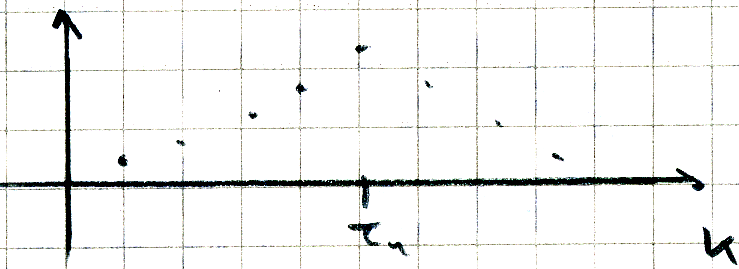
\includegraphics[width=1\textwidth]{./pics/MSTAT004.png}
		\caption{Plot von $\E[S_k]$}
		%\label{Abb}
	\end{center}
\end{figure}

Dies motiviert folgenden Schätzer (ersetze unbekannte $\big|\E[S_k)\big]$ durch bekannte $|S_k|$):
\begin{align*}
	\hat{\tau}_n:=\argmax\limits_{0\leq k\leq n}\big|S_k\big|
\end{align*}
Im Folgenden sei $\tau_n=\lfloor n\cdot\theta\rfloor,\theta\in(0,1)$.
Wir zeigen:
\begin{align*}
	\hat{\theta}_n:=\frac{\hat{\tau}_n}{n}\overset{n\to\infty}{\longrightarrow}\theta\qquad\P\text{-f.s.}
\end{align*}

\textbf{Annahme:} Wir nehmen die sogenannte \textbf{Momentenbedingung an}, d.h.
\begin{align*}
	\mu_p:=\E\Big[\big|X_{\tau_n}\big|^p\Big]<\infty,
	\qquad
	\nu_p:=\E\Big[\big|X_{\tau_n+1}\big|^p\Big]<\infty
\end{align*}

Sei $M_n:=$ Polygonzug durch $\left(\frac{k}{n},\frac{1}{n}\cdot S_k\right)$, $0\leq k\leq n$.
Dann folgt aus Lemma \ref{lemma7.17}:
\begin{align*}
	\hat{\theta}_n&:=\argmax\limits_{0\leq t\leq 1}\big|M_n(t)\big|\\
	M_n(t)&~=\frac{1}{n}\cdot S_{\lfloor n\cdot t\rfloor}+\big(n\cdot t-\lfloor w\cdot t\rfloor\big)\cdot\Big(S_{\lfloor n\cdot t\rfloor+1}-S_{\lfloor n\cdot t\rfloor+1}\Big) &\forall 0\leq t\leq 1\\
	\E\big[M_n(t)\big]&~=\frac{1}{n}\cdot\E\Big[ S_{\lfloor n\cdot t\rfloor}\Big]+\big(n\cdot t-\lfloor w\cdot t\rfloor\big)\cdot
	\Big(\E\Big[S_{\lfloor n\cdot t\rfloor+1}\Big]-\E\Big[S_{\lfloor n\cdot t\rfloor+1}\Big]\Big) &\forall 0\leq t\leq 1\\
\end{align*}

Sei $\overline{M}_n(t):=\E\big[M_n(t)\big),0\leq t\leq 1$. 
Dann ist $\overline{M}_n$ ein Polygonzug durch die Punkte $\left(\frac{k}{n},\frac{1}{n}\cdot\E[S_k]\right)$ $0\leq k\leq n$.
Da wegen \eqref{eqUnder8.2_1} 
\begin{align*}
	\overline{M}_n\left(\frac{k}{n}\right)
	&=\frac{1}{n}\cdot\E\big[S_k\big]
	\overset{\eqref{eqUnder8.2_1}}
	=
	\left\lbrace\begin{array}{cl}
		\frac{k}{n}\cdot(1-\theta_n)\cdot(\mu-\nu) &\falls \frac{k}{n}\leq\frac{\tau_n}{n}=\theta_n\\
		\left(1-\frac{k}{n}\right)\cdot\theta_n\cdot(\mu-\nu), & \falls \frac{k}{n}>\theta_n
	\end{array}\right.
\end{align*}
folgt
\begin{align*}
	\overline{M}_n\left(t\right)
	&=\left\lbrace\begin{array}{cl}
		t\cdot(1-\theta_n)\cdot(\mu-\nu) &\falls t\leq\theta_n\\
		\left(1-t\right)\cdot\theta_n\cdot(\mu-\nu), & \falls \frac{k}{n}>\theta_n
	\end{array}\right.
\end{align*}
Beachte $\theta-\frac{1}{n}<\theta_n=\frac{\lfloor n\cdot\theta\rfloor}{n}=\theta$.
Eine Fallunterscheidung ($t\leq\theta_n$; $\theta_n<t\leq\theta$; $t>\theta$) liefert
\begin{align}\label{eqUnder8.2_2}\tag{2}
	\big\Vert\overline{M}_n-M\big\Vert
	&=\sup\limits_{0\leq t\leq 1}\Big|\overline{M}_n(t)-M(t)\Big|
	\leq 2\cdot|\mu-\nu|\cdot n^{-1}\overset{n\to\infty}{\longrightarrow}0\text{ wobei}\\\nonumber
	M(t)&=\left\lbrace\begin{array}{cl}
		t\cdot(1-\theta)\cdot(\mu-\nu) ,&\falls 0\leq t\leq\theta\\
		(1-t)\cdot\theta\cdot(\mu-\nu), &\falls \theta<t\leq 1
	\end{array}\right.\\\nonumber
	|M(t)|&=\left\lbrace\begin{array}{cl}
		t\cdot(1-\theta)\cdot|\mu-\nu| ,&\falls 0\leq t\leq\theta\\
		(1-t)\cdot\theta\cdot|\mu-\nu|, &\falls \theta<t\leq 1
	\end{array}\right.
\end{align}

\begin{figure}[H]
	\begin{center}
		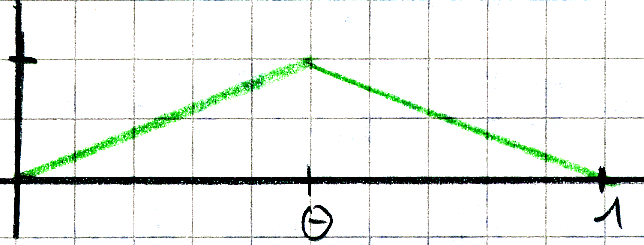
\includegraphics[width=1\textwidth]{./pics/MSTAT005.png}
		\caption{Plot von $M(t)$}
		%\label{AbbTitel}
	\end{center}
\end{figure}

Somit ist dieses $\theta$ charakterisierbar als Maximalstelle:
\begin{align*}
	\theta=\argmax\limits_{0\leq t\leq 1}\big|M(t)\big|
\end{align*}

Zeige:
\begin{align*}
	\big\Vert M_n-M\big\Vert
	&=\sup\limits_{0\leq t\leq 1}\big|M_n(t)-M(t)\big|\overset{n\to\infty}{\longrightarrow}0\quad\P\text{-f.s.}
\end{align*}
Da
\begin{align}\label{eqUnder8.2_3}\tag{3}
	0\leq\big\Vert M_n-M\big\Vert\leq\big\Vert M_n-\overline{M}_n\big\Vert+\underbrace{\big\Vert\overline{M}_n-M\big\Vert}_{
		\stackrelnew{\eqref{eqUnder8.2_2}}{n\to\infty}{\longrightarrow}0
	}
\end{align}

Betrachte den ersten Summanden
\begin{align}\label{eqUnder8.2_4}\tag{4}
	\big\Vert M_n-\overline{M}_n\big\Vert
	=\sup\limits_{0\leq t\leq 1}&\big|M_n(t)-\overline{M}_n(t)\big|
	\overset{\ref{lemma7.17}}{=}
	\max\limits_{0\leq k\leq n}\bigg|\underbrace{M_n\left(\frac{k}{n}\right)}_{=\frac{1}{n}\cdot S_k}-\underbrace{\overline{M}_n\left(\frac{k}{n}\right)}_{=\frac{1}{n}\cdot\E[S_k]}\bigg|\\\nonumber
	\frac{1}{n}\cdot S_k
	&=\frac{1}{n}\cdot\sum\limits_{i=1}^k\big(X_i-\overline{X}_n\big)
	=\frac{1}{n}\cdot\sum\limits_{i=1}^k X_i-\frac{k}{n^2}\cdot\sum\limits_{i=1}^n X_i\\\nonumber
	\implies
	M_n\left(\frac{k}{n}\right)-\overline{M}_n\left(\frac{k}{n}\right)
	\overset{\text{Lin}}&=
	\frac{1}{n}\cdot\sum\limits_{i=1}^n\underbrace{\Big(X_i-\E\big[X_i\big]\Big)}_{=:Z_i}-\frac{k}{n^2}\cdot\sum\limits_{i=1}^n\underbrace{\Big(X_i-\E\big[X_i\big]\Big)}_{=Z_i}\\\nonumber
	\implies
	\left|M_n\left(\frac{k}{n}\right)-\overline{M}_n\left(\frac{k}{n}\right)\right|
	\overset{\text{DU}}&\leq
	\frac{1}{n}\cdot\underbrace{\bigg|\sum\limits_{i=1}^n\underbrace{\Big(X_i-\E\big[X_i\big]\Big)}_{=:Z_i}\bigg|}_{
		\leq\max\limits_{0\leq k\leq n}\left|\sum\limits_{i=1}^k Z_i\right|
	}+\underbrace{\frac{k}{n^2}}_{\leq\frac{1}{n}}\underbrace{\cdot\bigg|\sum\limits_{i=1}^n\underbrace{\Big(X_i-\E\big[X_i\big]\Big)}_{=Z_i}\bigg|}_{
		\leq\max\limits_{0\leq k\leq n}\left|\sum\limits_{i=1}^k Z_i\right|
	}\\\nonumber
	&\leq2\cdot\frac{1}{n}\cdot\max\limits_{0\leq k\leq n}\left|\sum\limits_{i=1}^k Z_i\right|\\
	\implies\label{eqUnder8.2_5}\tag{5}
	&\max\limits_{0\leq k\leq n}\left|M_n\left(\frac{k}{n}\right)-\overline{M}_n\left(\frac{k}{n}\right)\right|
	\leq 2\cdot\frac{1}{n}\cdot\max\limits_{0\leq k\leq n}\left|\sum\limits_{i=1}^k Z_i\right|
\end{align}

Es ist
\begin{align*}
	T_k=\sum\limits_{i=1}^k Z_i\qquad 0\leq k\leq n
\end{align*}
ein Martingal bzgl. Filtration 
\begin{align*}
	\F_k:=\sigma\big(Z_1,\ldots,Z_k\big) &\qquad\forall 1\leq k\leq n,\qquad \F_0:=\lbrace\emptyset,\Omega\rbrace
\end{align*}
Ist Martingal, weil
\begin{align*}
	\E\Big[T_{k+1}~\Big|~\F_k\Big]
	&=\E\left.\left[\sum\limits_{i=1}^k Z_i+Z_{k+1}~\right|~\F_k\right]
	=\underbrace{\E\bigg[\overbrace{\sum\limits_{i=1}^k Z_i}^{\text{ist $\F_K$-messbar}}~\bigg|~\F_k\bigg]}_{=T_k}+\underbrace{\E\Big[ Z_{k+1}~\Big|~\F_k\Big]}_{=\E[Z_{k+1}]=0}
\end{align*}

Es folgt aus der bedingten Jensenungleichung, dass $\left(|T_k|^p,\F_k\right)_{0\leq k\leq n}$ ein nicht-negatives Submartingal ist.
\begin{align}\nonumber
	\P\Big(\big\Vert M_n-\overline{M}_n\big\Vert\geq\varepsilon\Big)
	\overset{\eqref{eqUnder8.2_4}+\eqref{eqUnder8.2_5}}&{\leq}
	2\cdot\frac{1}{n}\cdot\max\limits_{0\leq k\leq n}\big|T_k\big|\\\nonumber
	&\leq\P\left(\max\limits_{0\leq k\leq n}\big|T_k\big|\geq\frac{1}{2}\cdot n\cdot\varepsilon\right)\\\nonumber
	\overset{u\mapsto u^p\uparrow}&\leq
	\P\left(\left(\max\limits_{0\leq k\leq n}\big|T_k\big|\right)^p\geq\left(\frac{1}{2}\cdot n\cdot\varepsilon\right)^p\right)\\\nonumber
	&=\P\left(\max\limits_{0\leq k\leq n}\big|T_k\big|^p\geq\left(\frac{1}{2}\cdot n\cdot\varepsilon\right)^p\right)\\\nonumber
	\implies
	\P\Big(\big\Vert M_n-\overline{M}_n\big\Vert\geq\varepsilon\Big)
	&\leq\P\bigg(\max\limits_{0\leq k\leq n}\underbrace{\big|T_k\big|^p}_{\text{Submartingal}}\geq\underbrace{2^{-p}\cdot n^p\cdot\varepsilon^p}_{=:y>0}\bigg)\\\nonumber
	\overset{\text{Doob-Ungl}}&\leq
	y^{-1}\cdot\E\left[\big|T_n\big|^p\right]\\
	&=2^p\cdot n^{-p}\cdot\varepsilon^{-p}\cdot\E\left[\left|\sum\limits_{i=1}^n Z_i\right|^p\right]\label{eqUnder8.2_6}\tag{6}
\end{align}

Es gilt folgende \textbf{Momenten-Ungleichung} (vergleiche (1.6) in Ferger (2014), \textit{Optimal constants in the Marcinkiewicz-Zygmund-inequalities, statistics and propability letters} Ausgabe 84, Seiten 96 bis 101)

\begin{align*}
	\E\left[\left|\sum\limits_{i=1}^n Z_i\right|^p\right]
	\overset{(1.6)}{\leq}
	C_p\cdot n^{\frac{p}{2}}\cdot\sum\limits_{i=1}^n\E\Big[|Z_i|^p\Big]
\end{align*}

Erinnerung:
\begin{align*}
	Z_i&=X_i-\E[X_i]\\
	\implies
	|Z_i|^p&=\big|X_i-\E[X_i]\big|^p\\
	\implies
	\big|X_i-\E[X_i]\big|^p
	\overset{C_r\text{ Ungl}}&\leq
	c_p\cdot\Big(|X_i|^p+\underbrace{\big|\E[X_i]\big|^p}_{\overset{\text{Jensen}}{\leq}\E\big[|X_i|^p\big]}\Big)\\
	\implies
	\E\Big[|Z_i|^p\Big]
	&\leq c_p\cdot\left(\E\big[|X_i|^p\big]+\E\big[|X_i|^p\big]\right)\\
	&\leq 2\cdot c_p\cdot\underbrace{\E\Big[|X_i|^p\Big]}_{\leq\max\lbrace\mu_p,\nu_p\rbrace}
\end{align*}
Somit gibt es eine Konstante $D_p$ so, dass
\begin{align*}
	\E\left[\left|\sum\limits_{i=1}^n Z_i\right|^p\right]
	\overset{(1.6)}&{\leq}
	C_p\cdot n^{-\frac{p}{2}}\cdot\sum\limits_{i=1}^n\underbrace{\E\Big[|Z_i|^p\Big]}_{\leq D_p}\\
	\implies
	\E\left[\left|\sum\limits_{i=1}^n Z_i\right|\right]
	&\leq\tilde{c}_p\cdot n^{\frac{p}{2}}\\
	\overset{\eqref{eqUnder8.2_6}}{\implies}
	\P\Big(\big\Vert M_m-\overline{M}_n\big\Vert\geq\varepsilon\Big)
	&\leq\overline{c}_p\cdot\varepsilon^{-p}\qquad\forall\varepsilon>0
\end{align*}

Nun bilden wir die Reihe dieser Wahrscheinlichkeiten und erhalten Konvergenz für $p>2$:
\begin{align*}
	\overset{p>2}{\implies}
	\sum\limits_{n=1}^\infty\P\Big(\big\Vert M_m-\overline{M}_n\big\Vert\geq\varepsilon\Big)<\infty\qquad\forall\varepsilon>0
\end{align*}

Es gilt ganz allgemein für eine Folge $(\xi_n)_{n\in\N}$ von Zufallsvariablen (folgt aus dem Borel-Cantelli-Lemma):
\begin{align*}
	\left(\forall\varepsilon>0:\sum\limits_{n=1}^\infty\P\Big(|\xi_n|\geq\varepsilon\Big)<\infty\right)\implies\xi_n\overset{n\to\infty}{\longrightarrow}0\text{ f.s.}
\end{align*}

Also erhalten wir
\begin{align*}
	\big\Vert M_n-\overline{M}_n\big\Vert\overset{n\to\infty}{\longrightarrow}0\text{ f.s.}\\
	\overset{\eqref{eqUnder8.2_2}+\eqref{eqUnder8.2_3}}{\implies}
	\big\Vert M_n-M\big\Vert\overset{n\to\infty}{\longrightarrow}0\text{ f.s.}
\end{align*}

Da
\begin{align*}
	\Big\Vert\big|M_n\big|-\big|M\big|\Big\Vert\leq\big\Vert M_n-M\big\Vert
\end{align*}
folgt
\begin{align*}
	\Big\Vert\big|M_n\big|-\big|M\big|\Big\Vert\overset{n\to\infty}&{\longrightarrow}0\text{ f.s.}\\
	\implies	
	\Big\Vert-\big|M_n\big|-\big(-\big|M\big|)\Big\Vert\overset{n\to\infty}&{\longrightarrow}0\text{ f.s.}\\
	\implies
	\hat{\theta}_n
	&=\argmax\limits_{0\leq t\leq 1}\big|M_n(t)\big|
	=\argmin\limits_{0\leq t\leq 1}-\big|M_n(t)\big|
\end{align*}
Also hat $-|M|$ eindeutige Minimalstelle $\theta$.
Aus Satz \ref{satz8.6} folgt nun $\hat{\theta}\overset{n\to\infty}{\longrightarrow}\theta$ f.s.\\
(In Satz \ref{satz8.6} verwende: $M_n\hat{=}-|M_n|$, $M\hat{=}|M|$, $\tau\hat{=}\theta$)

\begin{bemerkung}
	Betrachte eine endliche Beobachtungsfolge:\\
	$X_1,X_2,\ldots,X_\tau,X_{\tau+1},X_{\tau+},\ldots,X_n\qquad n>\tau$\\
	Hier braucht man keinen doppelten Index.
	Vergrößert man aber nun $n$, dann geht der Anteil an der Gesamtstichprobe gegen 0, also $\frac{\tau}{n}\longrightarrow0$.
\end{bemerkung}

Zusammenfassung unserer Überlegungen in
\begin{satz}\label{satz8.8}
	Sei $\theta\in(0,1),\mu\neq\nu,\mu_p<\infty,\nu_p<\infty$ für ein $p>2$.
	Dann gilt:
	\begin{align*}
		\hat{\theta}_n
		&=\frac{1}{n}\cdot\underbrace{\argmax\limits_{0\leq k\leq n}\left|\sum\limits_{i=1}^k\big(X_i-\overline{X}_n\big)\right|}_{=\hat{\tau}_n}\overset{n\to\infty}{\longrightarrow}0\text{ f.s.}
	\end{align*}
\end{satz}

\begin{bemerkung}
	 Es gilt \underline{nicht}, dass $\hat{\tau}_n-\tau_n\overset{n\to\infty}{\longrightarrow}0$ f.s.
	 Tatsächlich gilt:
	 \begin{align*}
	 	\hat{\tau}_n-\tau_n\overset{\L}{\longrightarrow} T
	 \end{align*}
	 wobei $T$ die f.s. eindeutige Maximalstelle einer \textit{2-seitigen Irrfahrt / Random Walk} auf $\Z$ ist
	 (vergleiche D.F. (1994) \textit{Asymptotic distribution theory of change-point estimators} veröffentlicht in \textit{Mathematical methods in statics 3}, Seiten 362 bis 378).
\end{bemerkung}

Nächstes Ziel: Unter welchen Bedingungen gilt
\begin{align*}
	Z_n\overset{L}{\longrightarrow}Z\text{ in }\big(C(\R),d\big)
	\implies\argmin\limits_{t\in\R}Z_n(t)\overset{\L}{\longrightarrow}\argmin\limits_{t\in\R}Z(t)
\end{align*}

Folgender Satz gibt Antwort.

\begin{satz}\label{satz8.9}
	Seien $Z,Z_n,n\in\N$ stochastische Prozesse mit Pfaden in $C(\R)$ über $(\Omega,\A,P)$,
	wobei $A(Z)$ 
	\footnote{$A(Z)$ ist eine \textit{random closed set (RCS)}} 
	und $A(Z_n)$ für alle $n\in\N$ nichtleer sind.
	Ferner sei $\sigma_n$ eine Zufallsvariable mit $\sigma_n\in A(Z_n)$.
	Dann gilt: Falls
	\begin{align}\label{eqSatz8.9_1}\tag{1}
		Z_n\overset{L}{\longrightarrow} Z\text{ in }\big(C(\R),d\big)
	\end{align}
	so folgt
	\begin{align}\label{eqSatz8.9_a}\tag{a}
		\limsup\limits_{n\to\infty}\P\big(\sigma_n\in K\big)\leq\mu^\ast(K)\qquad\forall K\in\mathcal{K}:=\big\lbrace K\subseteq\R:K\text{ kompakt}\big\rbrace
	\end{align}
	wobei $\mu^\ast$
	\footnote{$\mu^\ast$ ist die \textit{Kapazitätsfunktion von $A(Z)$} und damit insbesondere eine \textit{Choquet-Kapazität}.
	Beachte, dass $\mu^\ast$ i.d.R. \underline{kein} W-Maß.}	
	die sogenannte \textbf{hitting-probability} ist:
	\begin{align*}
		\mu^\ast:\mathcal{K}\to[0,1],\qquad
		\mu^\ast(K)=\P\big(A(Z)\cap K\neq\emptyset\big)
	\end{align*}
	Gilt zusätzlich, dass $(\sigma_n)_{n\in\N}$ \textbf{stochastisch beschränkt} ist, d.h. 
	\begin{align}\label{eqSatz8.9_2}\tag{2}
		\lim\limits_{j\to\infty}\limsup\limits_{n\to\infty}\P\Big(\big|\sigma_n\big|>j\Big)=0
	\end{align}
	so folgt
	\begin{align}\label{eqSatz8.9_b}\tag{b}
		\limsup\limits_{n\to\infty}\P\big(\sigma_n\in F\big)\leq\mu^\ast(F)\qquad\forall F\in\F(\R):=\big\lbrace F\subseteq\R:F\text{ abgeschlossen}\big\rbrace
	\end{align}
	Falls zusätzlich $A(Z)=\lbrace\sigma\rbrace$ für eine Zufallsvariable $\sigma$
	(d.h. $Z$ hat f.s. eine eindeutige Minimalstelle, nämlich $\sigma$), dann gilt
	\begin{align}\label{eqSatz8.9_c}\tag{c}
		\sigma_n\overset{L}{\longrightarrow}\sigma\text{ in }\R.
	\end{align}
\end{satz}

%Ferger: "Ich weiß nicht mehr wie ich drauf gekommen bin. Aber ich bin darauf gekommen. Da habe ich mich gefreut wie so ein Brötchen."
%Ferger: "Müssen Sie nicht mitschreiben, ich will jetzt hier nur zu einer didaktischen Meisterleistung auflaufen."

\begin{proof}
	\underline{Zeige \eqref{eqSatz8.9_a}:}\\
	Sei $K$ kompakt. Dann gilt:
	\begin{align}\label{eqProofSatz8.9_i}\tag{i}
		\big\lbrace\sigma_n\in K\big\rbrace
		&\subseteq\left\lbrace\inf\limits{t\in K} Z_n(t)\leq\inf\limits_{t\not\in K} Z_n(t)\right\rbrace\\
		&\subseteq\left\lbrace\inf\limits_{t\in K} Z_n(t)\leq\inf\limits_{t\in K^C\cap I_j}Z_n(t)\right\rbrace\label{eqProofSatz8.9_ii}\tag{ii}
	\end{align}
	wobei $I_j:=[-j,j],j\in\N$.\nl
	\underline{Zeige \eqref{eqProofSatz8.9_i}:}\\
	Sei $\sigma_n\in K$ und angenommen
	\begin{align}\label{eqProofSatz8.9Stern}\tag{$\ast$}
		\inf\limits_{t\in K} Z_n(t)>\inf\limits_{t\in K^C} Z_n(t)
	\end{align}
	Dann gilt:
	\begin{align*}
		Z_n(\sigma_n)
		\overset{\sigma_n\in K}&\geq
		\inf\limits_{t\in K} Z_n(t)
		\overset{\eqref{eqProofSatz8.9Stern}}>
		\inf\limits_{t\in K^C} Z_n(t)
		\overset{K^C\subseteq\R}\geq
		\inf\limits_{t\in\R} Z_n(t)
		\overset{\sigma_n\in A(Z_n)}=
		Z(\sigma_n)
	\end{align*}
	Das ist ein Widerspruch, weshalb \eqref{eqProofSatz8.9_i} folgt.\nl
	Gleichung \eqref{eqProofSatz8.9_ii} folgt aus 
	\begin{align*}
		\inf\limits_{t\in K^C} Z_n(t)\leq\inf\limits_{t\in K^C\cap I_j}Z_n(t).
	\end{align*}
	Sei $K_j:=[-k_j,k_j]$ mit $k_j\in\N$ so, dass $K_j\supseteq K\cup I_j$.
	Für jedes $M\subseteq K_j$ gilt:
	Die Abbildung $f\mapsto\inf\limits_{t\in M} f(t)$ ist stetig auf $\big(C(K_j),\Vert\cdot\Vert_{K_j}\big)$,
	denn:
	\begin{align*}
		\left|\inf\limits_{t\in M} f(t)-\inf\limits_{t\in M}g(t)\right|
		&\leq \Vert f-g\Vert_M
		\leq\Vert f-g\Vert_{K_j}
	\end{align*}
	Daraus folgt, dass die Abbildung
	\begin{align*}
		H_j:\left(C\big(K_j\big),\Vert\cdot\Vert_{K_j}\right)\to\R,\qquad
		f\mapsto\inf\limits_{t\in K} f(t)-\inf\limits_{t\in K^C\cap I_j} f(t)
	\end{align*}
	stetig ist, denn $K^C\cap I_j\subseteq I_j\subseteq K\cup I_j\subseteq K_j$.
	Somit folgt aus Satz \ref{satz7.23} und aus dem CMT \ref{satz4.10ContinuousMappingTheorem}:
	\begin{align}\label{eqProofSatz8.9_iii}\tag{iii}
		H_j(Z_n)\overset{\L}{\longrightarrow} H_j(Z)\qquad\forall j\in\N
	\end{align}
	Aus \eqref{eqProofSatz8.9_i} und \eqref{eqProofSatz8.9_ii} folgt:
	\begin{align}\nonumber
		\P\Big(\big\lbrace\sigma_n\in K\big\rbrace\Big)
			&\leq\P\Bigg(\Bigg\lbrace\underbrace{\inf\limits_{t\in K} Z_n(t)-\inf\limits_{t\in K^C\cap I_j}Z_n(t)}_{=H_j(Z_n)}\leq0\Bigg\rbrace\Bigg)\\\nonumber
		\implies		
		\limsup\limits_{n\to\infty}\P\big(\sigma_n\in K\big)
		\overset{\eqref{eqProofSatz8.9_i}+\eqref{eqProofSatz8.9_ii}}&\leq
		\limsup\limits_{n\to\infty}\P\Big(H_j(Z_n)\in\underbrace{(-\infty,0]}_{\in\F(\R)}\Big)\\\nonumber
		\overset{\eqref{eqProofSatz8.9_iii}+\text{Portmannteau}}&\leq
		\P\Big(H_j(Z)\in(-\infty,0]\Big)\\
		\overset{\text{Def }H_j}&=
		\P\bigg(\underbrace{\bigg\lbrace\inf\limits_{t\in K}Z(t)\leq\inf\limits_{t\in K^C\cap I_j}Z(t)\bigg\rbrace}_{=:E_j}\qquad\forall j\in\N\label{eqProofSatz8.9_iv}\tag{iv}
	\end{align}
	Da $E_j$ monoton fallend ist, folgt (mit $\sigma$-Stetigkeit von oben):
	\begin{align*}
		\lim\limits_{j\to\infty}\P(E_j)
		&=\P\left(\bigcap\limits_{j\in\N}E_j\right)\\
		&=\P\left(\inf\limits_{t\in K}Z(t)\leq\inf\limits_{t\in K^C\cap I_j}Z(t)~\forall j\in\N\right)\\
		&\leq \P\bigg(\inf\limits_{t\in K}Z(t)\leq\underbrace{\inf\limits_{j\in\N}\inf\limits_{t\in K^C\cap I_j}Z(t)}_{=\inf\limits_{\bigcup\limits_{j\in\N}\big(K^C\cap I_j\big)}Z(t)}\bigg)\\
		\overset{\bigcup\limits_j(K^C\cap I_j)=K^C\cap\bigcap\limits_j I_j=K^C\cap\R}&=
		\P\bigg(\underbrace{\bigg\lbrace\inf\limits_{t\in K} Z(t)\leq\inf\limits_{t\in K^C} Z(t)\bigg\rbrace}_{=:E}\bigg)
	\end{align*}
	Dahinter steckt die allgemeine Rechenregel
	\begin{align*}
		\inf\limits_{t\in A\cup B}f(t)=\inf\limits\left\lbrace\inf\limits_A f,\inf\limits_B f\right\rbrace.
	\end{align*}
	Grenzübergang $j\to\infty$ in \eqref{eqProofSatz8.9_iv} liefert:
	\begin{align}\label{eqProofSatz8.9Plus}\tag{+}
		\limsup\limits_{n\to\infty}\P\big(\sigma_n\in K\big)
		\leq\lim\limits_{j\to\infty}\P(E_j)\leq\P(E)
	\end{align}
	Schließlich gilt
	\begin{align}\label{eqProofSatz8.9_v}\tag{v}
		E\subseteq\big\lbrace A(Z)\cap K\neq\emptyset\big\rbrace
	\end{align}
	denn:
	\begin{align*}
		&\inf\limits_{t\in K}Z(t)
		\leq\inf\limits_{t\in K^C} Z(t)\\
		&\implies
		\inf\limits_\R Z(t)=\inf\limits_{K\cup K^C}Z(t)=\min\left\lbrace\inf\limits_{t\in K} Z(t),\inf\limits_{t\in K^C}Z(t)\right\rbrace=\inf_{t\in K}Z(t)
		=Z(\tau)
	\end{align*}
	für ein $\tau\in K$, da $Z$ stetig und $K$ kompakt.
	Also ist $\tau$ eine Minimalstelle von $Z$, i.Z. $\tau\in A(Z)$.
	Da $\tau\in K$ ist, gilt
	\begin{align*}
		\tau\in A(Z)\cap K\\
		\implies A(Z)\cap K\neq\emptyset
	\end{align*}
	Wegen \eqref{eqProofSatz8.9_v} gilt, dass
	\begin{align*}
		\P(E)\leq\P\big(A(Z)\cap K\neq\emptyset\big)=\mu^\ast(K)
	\end{align*}
	und \eqref{eqSatz8.9_a} folgt aus \eqref{eqProofSatz8.9Plus}.\nl
	\underline{Zeige \eqref{eqSatz8.9_b}:}\\
	Sei $F\in\F$. Dann gilt:
	\begin{align}\nonumber
		\big\lbrace\sigma_n\in F\big\rbrace
		\overset{\text{Zerlegung}}&=
		\big\lbrace\sigma_n\in F,\sigma_n\in I_j\big\rbrace
		\dot{\cup}\big\lbrace\sigma_n\in F,\sigma_n\not\in I_j\big\rbrace\\\nonumber
		&=\big\lbrace\sigma_n\in \underbrace{F\cap I_j}_{\text{kompakt}}\big\rbrace\dot{\cup}\big\lbrace |\sigma_n|>j\big\rbrace&\forall& j\in\N\\\nonumber
		\implies
		\P\Big(\big\lbrace\sigma_n\in F\big\rbrace\Big)
		&\leq\P\Big(\big\lbrace\sigma_n\in F\cap I_j\big\rbrace\Big)+\P\Big(\big\lbrace |\sigma_n|>j\big\rbrace\Big)&\forall& j\in\N\\
		\limsup\limits_{n\to\infty}\P(\sigma_n\in F)
		&\leq\underbrace{\limsup\limits_{n\to\infty}\P\big(\sigma_n\in F\cap I_j)}_{
			\overset{\eqref{eqSatz8.9_a}}{\leq}\P\big(\underbrace{\big\lbrace A(Z)\cap(F\cap I_j)\neq\emptyset\big\rbrace}_{=:B_j}
		}+\underbrace{\limsup\limits_{n\to\infty}\P\big(|\sigma_n|>j\big)}_{
			\overset{j\to\infty}{\longrightarrow}\text{ wegen }\eqref{eqSatz8.9_2}
		} &\forall& j\in\N\label{eqProofSatz8.9PlusPlus}\tag{++}
	\end{align}
	Da
	\begin{align*}
		B_j\uparrow\big\lbrace A(Z)\cap F\neq\emptyset\big\rbrace
	\end{align*}
	 (zur Übung), liefert Grenzübergang $j\to\infty$ in \eqref{eqProofSatz8.9PlusPlus} und $\sigma$-Stetigkeit von unten und \eqref{eqSatz8.9_2} die Behauptung \eqref{eqSatz8.9_b}.\nl
	 \underline{Zeige \eqref{eqSatz8.9_c}:}
	 \begin{align*}
	 	&A(Z)=\lbrace\sigma\rbrace\text{ f.s.}\\
	 	&\implies\mu^\ast(F)=\P\big(A(Z)\cap F\neq\emptyset\big)
	 	=\P\Big(\big\lbrace\sigma\rbrace\cap F\neq\emptyset\big\rbrace\Big)
	 	=\P(\sigma\in F)\\
	 	\overset{\eqref{eqSatz8.9_b}}&\implies
	 	\limsup\limits_{n\to\infty}\P\big(\sigma_n\in F\big)\leq\mu^\ast(F)
	 	=\P(\sigma\in F)\qquad\forall F\in F\\
	 	\overset{\text{Portmannteau}}&{\implies}
	 	\sigma_n\overset{\L}{\longrightarrow}\sigma
	 \end{align*}
\end{proof}

%Ferger: "Ich war früher so ein richtiger Sport-Paul. Aber jetzt bin ich einfach zu faul. Ist nicht so, dass ich keine Zeit habe.

\subsection{Anwendung}

Sei $X_1,\ldots,X_n$ i.i.d. Kopien von $X$ mit $\mu$-Dichte 
\begin{align*}
	f_\theta(x)&=c(\theta)\cdot h(x)\cdot\exp\big(q(\theta)\cdot T(x)\big)\qquad\forall x\in\X,\forall\theta\in\Theta=\R
\end{align*}
Sei $\theta_0$ der wahre Parameter.
Dann gilt:

\begin{align}\label{eqAnwendung_1}\tag{1}
	\text{MLS $\hat{\theta}_n$ für $\theta$ ist }\hat{\theta}_n&=\argmin\limits_{t\in\R}M_n(t)\qquad\mit\\
	M_n(t)&=-\log\big(c(t)\big)-q(t)\cdot\overline{T}_n,\qquad
	\overline{T}_n=\frac{1}{n}\cdot\sum\limits_{i=1}^nt(X_i)\nonumber
\end{align}
Ziel: Nachweis von
\begin{align*}
	\sqrt{n}\cdot\big(\hat{\theta}_n-\theta_0\big)\overset{\L}{\longrightarrow}\xi
\end{align*}
und Identifizierung von $\xi$.\nl
Dazu: Sei 
\begin{align*}
	Z_n(t):=n\cdot\left(M_n\left(\theta_0+\frac{t}{\sqrt{n}}\right)-M_n\big(\theta_0\big)\right)\qquad\forall t\in\R
\end{align*}
der \textbf{reskalierte Prozess} zu $M_n$.
Offenbar ist $Z_n$ stetiger stochastischer Prozess \underline{und}
\begin{align}\label{eqAnwendung_2}\tag{2}
	\underbrace{\sqrt{n}\cdot\big(\hat{\theta}_n-\theta\big)}_{=:\sigma_n}
	&=\argmin\limits_{t\in\R} Z_n(t)
\end{align}
denn:
Zu zeigen: 
\begin{align*}
	Z_n(\sigma_n)\leq Z_n(t)\qquad\forall t\in\R
\end{align*}
Dazu nutze Äquivalenzen:
\begin{align*}
	&Z_n(\sigma_n)\leq Z_n(t) &\forall& t\in\R\\
	\overset{t=\sigma_n}&\Longleftrightarrow
	n\bigg(M_n\cdot\bigg(\underbrace{\theta_0+\frac{\sigma_n}{\sqrt{n}}}_{
		\begin{subarray}{c}
			=\theta_0+\frac{\sqrt{n}\big(\hat{\theta}_n-\theta_n\big)}{\sqrt{n}}\\
			=\theta_n
		\end{subarray}
	}\bigg)-M_n(\theta_0)\bigg)
	\leq n\cdot\left(M_n\left(\theta_0+\frac{t}{\sqrt{n}}\right)-M_n(\theta_0)\right)&\forall& t\in\R\\
	&\Longleftrightarrow n\cdot\Big(M_n\big(\hat{\theta}_n\big)-M_n\big(\theta_0\big)\Big)
	\leq n\cdot\left(M_n\left(\theta_0+\frac{t}{\sqrt{n}}\right)-M_n(\theta_0)\right) &\forall&t\in\R\\
	&\Longleftrightarrow M_n\big(\hat{\theta}_n\big)
	\leq M_n\left(\theta_0+\frac{t}{\sqrt{n}}\right) &\forall&t\in\R\\
	&\Longleftrightarrow M_n\big(\hat{\theta}_n\big)
	\leq M_n\left(\theta_0+\frac{t}{\sqrt{n}}\right) &\forall& t\in\R\\
	&\Longleftrightarrow M_n\big(\hat{\theta}_n\big)\leq M_n(u) &\forall& u\in\R\\
	\overset{\eqref{eqAnwendung_1}}&\Longleftrightarrow \text{ True}
\end{align*}
Wegen \eqref{eqAnwendung_2} versuche Satz \ref{satz8.9} anzuwenden:\\
Man kann zeigen:
\begin{align}\label{eqAnwendung_i}\tag{i}
	Z_n\overset{\L}{\longrightarrow} Z\text{ in }\big(C(\R),d\big)
\end{align}
wobei
\begin{align*}
	Z(t)
	&=-q'(\theta_0)\cdot N\cdot t+\frac{1}{2}\cdot\big(q'(\theta_0)\big)^2\cdot\sigma^2(\theta_0)\cdot t^2 \qquad\forall t\in\R
\end{align*}
wobei wir fordern:
\begin{align*}
	\sigma^2(\theta_0):=\Var_{\theta_0}\big(T(X)\big)\overset{\text{Forderung}}&>0\\
	q'(\theta_0)\overset{\text{Forderung}}&\neq0\\
	N&\sim\Nor\big(0,\sigma^2(\theta_0)\big)
\end{align*}
Also ist $Z$ eine zufällige nach oben geöffnete Parabel.

\begin{align*}
	0
	&=Z'(t)
	=-q'(\theta_0)\cdot N+\big(q'(\theta_0)\big)^2\cdot\sigma^2(\theta_0)\cdot t\\
	\xi
	&=\frac{1}{q'(\theta_0)\cdot\sigma^2(\theta_0}\cdot N
	\text{ ist die eindeutige Minimalstelle von }Z.
\end{align*}
Man kann zeigen:
\begin{align*}
	\limsup\limits_{n\to\infty}\P\Big(\sqrt{n}\cdot\big|\hat{\theta}_n-\theta_0\big|\geq j\Big)
	\leq\frac{4}{\big(q'(\theta_0)\big)^2\cdot\sigma^2(\theta_0)}\cdot\frac{1}{j^2}\qquad\forall n\in\N
\end{align*}
Grenzübergang $j\to\infty$ liefert, dass zweite Bedingung \eqref{eqSatz8.9_2} in Satz \ref{satz8.9} erfüllt ist.
Somit liefert Satz \ref{satz8.9}:
\begin{align*}
	\sqrt{n}\cdot\big(\hat{\theta}_n-\theta_0\big)\overset{\L}{\longrightarrow}\xi
\end{align*}

	% This work is licensed under the Creative Commons
% Attribution-NonCommercial-ShareAlike 4.0 International License. To view a copy
% of this license, visit http://creativecommons.org/licenses/by-nc-sa/4.0/ or
% send a letter to Creative Commons, PO Box 1866, Mountain View, CA 94042, USA.

\section{Verteilungskonvergenz im Raum konvexer Funktionen} %9

\begin{definition}\label{def9.1}\
	\begin{enumerate}[label=(\arabic*)]
		\item Eine Menge $\emptyset\neq O\subseteq\R$ heißt \textbf{konvex}
		\begin{align*}
			:\Longleftrightarrow x,y\in O\implies\forall\lambda\in(0,1):\lambda\cdot x+(1-\lambda)\cdot y\in O
		\end{align*}
		\item Sei $O$ konvex. Eine Funktion $f\colon O\to\R$ heißt \textbf{konvex}
		\begin{align*}
			:\Longleftrightarrow 
			f\big(\lambda\cdot x+(1-\lambda)\cdot y\big)\leq\lambda\cdot f(x)+(1-\lambda)\cdot f(y)\qquad\forall x,y\in,\forall\lambda\in(0,1)
		\end{align*}
		\item $\begin{aligned}
			C_c(O):=\big\lbrace f\colon O\to\R:f\text{ konvex}\big\rbrace
		\end{aligned}$
		\item Ein stochastischer Prozess
		\begin{align*}
			X=\big\lbrace X(t):t\in O\big\rbrace
		\end{align*}				
		über $(\Omega,\A)$ mit Pfaden in $C_c(O)$ heißt \textbf{konvexer stochastischer Prozess} auf $O$.
	\end{enumerate}
\end{definition}

Im Folgenden sei $O=(a,b)$ mit $-\infty\leq a<b\leq\infty$ und $d$ die Metrik der gleichmäßigen Konvergenz auf $C_c(O)$.
Bekanntlich ist $C_c(O)\subseteq C(O)$, also $\big(C_c(O),d\big)$ als Unterraum von $\big(C(O),d\big)$ ebensfalls separabel.
Seien $\pi_t$ und $\pi_T$ die Projektionen eingeschränkt auf $C_c(O)$.

\begin{satz}\label{satz9.2}
	\begin{align*}
		\B_d\big(C_c(O)\big)=\sigma\big(\pi_t:t\in O\big)=\sigma\big(\pi_T:T\subseteq O\text{ endlich}\big)
	\end{align*}
\end{satz}

\begin{proof}
	Analog zu Satz \ref{satz7.2}.
\end{proof}

%Ferger: "Ich bin zu gut für diese Welt." (also er einen Satz nochmals anschrieb, weil einige Stundenten nicht hinterher kamen)

Wir erhalten folgende Korollare:

\begin{korollar}\label{korollar9.3}
	 Sei $X$ konvexer stochastischer Prozess über $(\Omega,\A)$ auf $O$.\\
	 Dann ist die Pfadabbildung
	 \begin{align*}
	 	X\colon(\Omega,\A)\to\Big(\C_c(O),\B_d\big(C_c(O)\big)\Big)
	 \end{align*}
	 messbar.
\end{korollar}

\begin{korollar}\label{korollar9.4} %9.3 in VL
	Seien $X,Y$ Zufallsvariablen in $\big(C_c(O),d\big)$.
	Dann gilt:
	\begin{align*}
		X\overset{\L}{=} Y\Longleftrightarrow
		\big(X(t_1),\ldots,X(t_k)\big)
		\overset{\L}{=}
		\big(Y(t_1),\ldots,Y(t_k)\big)
		\qquad\forall t_1,\ldots,t_k\in O,\forall k\in\N
	\end{align*}
	(Die endlich dimensionalen Randverteilungen sind gleich.)
\end{korollar}

\begin{beispiel}\label{beispiel9.5}\
	\begin{enumerate}[label=(\arabic*)]
		\item $f(x):=|x|,x\in\R$ ist konvex.
		\begin{proof}
			Folgt aus Dreiecksungleichung.
		\end{proof}
		\item Sei $f\colon\R\to\R$ konvex und $a\in\R$.
		Dann ist auch $f_a(x):=f(x-a),x\in\R$ konvex.
		\begin{proof}
			Nachrechnen.
		\end{proof}
	\end{enumerate}
\end{beispiel}

\begin{lemma}\label{lemma9.6}
	Sei $F$ Verteilungsfunktion auf $\R$ mit
	\begin{align*}
		\int\limits_\R |x|~F(\d x)<\infty
	\end{align*}
	Dann ist die Funktion
	\begin{align*}
		M\colon\R\to\R,\qquad M(t):=\int\limits_\R|x-t|~F(\d x)\qquad\forall t\in\R
	\end{align*}
	konvex.
\end{lemma}

\begin{proof}
	Folgt aus Beispiel \ref{beispiel9.5} und der Monotonie und Linearität des Integrals.
\end{proof}

Erinnere an:\\
$m$ ist \textbf{Median} von $F$
\begin{align*}
	:\Longleftrightarrow m\in A(M)
\end{align*}
$\hat{m}_n$ ist \textbf{empirischer Median} zu $X_1,\ldots,X_n$
\begin{align*}
	:\Longleftrightarrow&\hat{m}_n\in A(M_n)
	\qquad\mit\qquad
	\hat{M}_n(t):=\int\limits_\R|x-t| F_n(\d x)
\end{align*}
wobei $F_n$ die \textit{empirische Verteilungsfunktion} zu $X_1,\ldots,X_n$ ist.
Also:
\begin{align*}
	M_n(t)=\frac{1}{n}\cdot\sum\limits_{i=1}^n\big|X_i-t\big|\qquad\forall t\in\R
\end{align*}
Gemäß \ref{korollar9.3} sind $M_n,n\in\N$ und $M$ als	 konvexe stochastische Prozesse Zufallsvariablen in $\big(C_r(\R),d\big)$.

\begin{satz}\label{satz9.7}
	Sei $D\subseteq O$ dicht in $O=(a,b)\subseteq\R$ (z. B. $D=\Q\cap O$) und $K\subseteq O$ kompakt.
	Dann existieren eine universelle Konstante $c$ und Punkte $b_1,\ldots,b_m\in D$ so, dass für jede Konvexe Funktion $f\colon O\to\R$ gilt:
	\begin{align*}
		\big|f(x)-f(y)\big|\leq c\cdot\sum\limits_{i=1}^n\big|f(b_i)\big|\cdot|x-y|\qquad\forall x,y\in O
	\end{align*}
\end{satz}

\begin{proof}
	Siehe Liese und Mischka (2008) \textit{Statistical decision theory} Seite 402 bis 403.
\end{proof}

% Ferger: "Da sehe ich mich noch Samstagsmittags nach einem gut gekühlten Weißwein und blättere in dem Buch und stoße auf dieses Ergebnis. Da bin ich erst mal vor Freude hin und her gehopst."

\begin{theorem}\label{theorem9.8}
	Seien $f_n,n\in\N$ konvexe Funktionen auf $O$, $D\subseteq O$ dicht in $O$.
	Sei $f\colon O\to\R$ eine Funktion.
	Falls 
	\begin{align}\label{eqtheorem9.8Stern}\tag{$\ast$}
		f_n(x)\overset{n\to\infty}{\longrightarrow} f(x)\qquad\forall x\in D
	\end{align}
	gilt, so gilt:
	\begin{enumerate}[label=(\arabic*)]
		\item $\begin{aligned}
			f(x)=\limn f_n(x)\text{ existiert }\qquad\forall x\in O
		\end{aligned}$
		\item $f$ ist konvex.
		\item $\begin{aligned}
			\big\Vert f_n-f\big\Vert_K\overset{n\to\infty}{\longrightarrow}0\qquad\forall K\subseteq O
		\end{aligned}$
	\end{enumerate}
\end{theorem}

% Ferger kommt aus Westerwald, Westerburg

\begin{proof}
	Siehe Rockafellar (1972) \textit{Convex Analysis} Theorem 10.8.
\end{proof}

\begin{satz}\label{satz9.9}
	Seien $X_n,n\in\N$ konvexe stochastische Prozesse und sei $X$ stetiger stochastischer Prozess auf $\R$ über $(\Omega,\A,\P)$.
	Dann sind (1) $\gdw$ (2) $\implies$ (3):
	\begin{enumerate}[label=(\arabic*)]
		\item $\begin{aligned}
			X_n\overset{\text{fd}}{\longrightarrow}X\qquad\text{Konvergenz der fidis}
		\end{aligned}$
		\item $\begin{aligned}
			X_n\overset{\L}{\longrightarrow} X\text{ in }\big(C(\R),d\big)
		\end{aligned}$
		\item In jedem Fall ist $X$ ein \underline{konvexer} stochastischer Prozess.
	\end{enumerate}
\end{satz}

\begin{proof}
	\underline{Zeige (1) $\implies$ (2):}\\
	Gemäß Satz \ref{satz7.23} ist zu zeigen:
	\begin{align}\label{eqProofSatz9.9Stern}\tag{$\ast$}
		X_n^{(j)}\overset{\L}{\longrightarrow} X^{(j)}\text{ in }\big(C(I_j),d_j\big)\qquad\forall j\in\N\mit I_j:=[-j,j]
	\end{align}		
	Nachweis von \eqref{eqProofSatz9.9Stern} mit Satz \ref{satz7.9}.
	Voraussetzung (1) in Satz \ref{satz7.9} ist nach Voraussetzung erfüllt.
	Betrachte den \textbf{Oszillationsmodul}
	\begin{align*}
		q\left(X_n^{(ij)},\delta\right)
		\overset{\text{Def}}&=
		\sup\limits\Big\lbrace\big|X_n(s)-X_n(t)\big|:s,t\in I_j,|s-t|\leq\delta\Big\rbrace\\
		&\leq \underbrace{c\cdot\sum\limits_{i=1}^m\big|X_n(b_i)\big|}_{=:Z_n}\cdot\delta\mit c>0\text{ und }b_1,\ldots,b_m\in I_j
	\end{align*}
	
	Wegen (1) gilt 
	\begin{align*}
		X_n(b_1),\ldots,X_n(b_m)\big)\overset{\L}&{\longrightarrow}\big(X(b_1),\ldots,X(b_m)\big)\\
		\overset{\ref{satz4.10ContinuousMappingTheorem}}\implies
		Z_n\overset{\L}{\longrightarrow} Z&=c\cdot\sum\limits_{i=1}^m\big|X(b_i)\big|\\
		\implies
		0&\leq\limsup\limits_{n\to\infty}\P\Big(\underbrace{w\Big(X_n^{(j)},\delta_k\Big)}_{\leq Z_n\cdot\delta_k}\geq\varepsilon\Big)\\
		&\leq\limsup\limits_{n\to\infty}\P\left(Z_n\geq\frac{\varepsilon}{\delta_k}\right)\\
		\overset{\text{Portmannteau}}&\leq
		\P\left(Z\geq\frac{\varepsilon}{\delta_k}\right)
		\qquad\forall\varepsilon>0,\forall(\delta_k)_{k\in\N}\subseteq(0,\infty)
	\end{align*}
	Für $\delta_k\downarrow0$ folgt $\frac{\varepsilon}{\delta_k}\overset{k\to\infty}{\longrightarrow}+\infty$, also
	\begin{align*}
		\P\left(Z\geq\frac{\varepsilon}{\delta_k}\right)\overset{k\to\infty}{\longrightarrow}0
	\end{align*}
	Somit ist Voraussetzung (2) in Satz \ref{satz7.9} erfüllt. 
	Daraus folgt (2).\nl
	\underline{Zeige (2) $\implies$ (1):}
	Folgt direkt aus dem CMT \ref{satz4.10ContinuousMappingTheorem}.\nl
	\underline{Zeige (2) $\implies$ (3):} 
	Ohne Beweis.
\end{proof}

\begin{lemma}[Subspace-Lemma]\label{lemma9.10SubspaceLemma}\enter
	Sei $U\subseteq\S$ ein Unterraum des metrischen Raumes $(\S,d)$.
	Seien $Z,Z_n,n\in\N$ Zufallsvariablen in $\big(U,\B_d(U)\big)$.
	Dann gilt:
	\begin{align*}
		Z_n\overset{\L}{\longrightarrow} Z\text{ in }(\S,d)
		\Longleftrightarrow
		Z_n\overset{\L}{\longrightarrow} Z\text{ in }(U,d)
	\end{align*}
\end{lemma}

\begin{proof}
	Siehe Kallenberg (1997) \textit{Foundations of modern probability}, Lemma 3.2
\end{proof}

\begin{korollar}\label{korollar9.11}
	Seien $X,X_n,n\in\N$ konvexe stochastische Prozesse über $(\Omega,\A)$ auf $\R$ nach $\R$ mit 
	\begin{align*}
		X_n\overset{\text{fd}}{\longrightarrow}X
	\end{align*}
	Dann folgt
	\begin{align*}
		X_n\overset{\L}{\longrightarrow} X\text{ in }\big(C_c(\R),d\big)
	\end{align*}
\end{korollar}

\begin{proof}
	Folgt aus Satz \ref{satz9.9} und Lemma \ref{lemma9.10SubspaceLemma}.
\end{proof}
	% This work is licensed under the Creative Commons
% Attribution-NonCommercial-ShareAlike 4.0 International License. To view a copy
% of this license, visit http://creativecommons.org/licenses/by-nc-sa/4.0/ or
% send a letter to Creative Commons, PO Box 1866, Mountain View, CA 94042, USA.

\section{Argmin-Theoreme in \texorpdfstring{$C_c(\R)$}{C\_c(R)}} %10

\begin{lemma}\label{lemma10.1}
	Seien $f\colon\R^d\to\R$ konvex, $g\colon\R^d\to\R$ stetig, $A(f)\neq\emptyset$, $A(g)=\lbrace\sigma\rbrace$.\\
	Für $\varepsilon>0$ seien
	\begin{align*}
		\overline{B}(\sigma,\varepsilon)&:=\big\lbrace t\in\R^d:|t-\sigma|\leq\varepsilon\big\rbrace\\
		m(\varepsilon)&:=\inf\limits\big\lbrace g(t9:|t-\sigma|=\varepsilon\big\rbrace\\
		b(\varepsilon)&:=\frac{1}{2}\cdot\big(m(\varepsilon)-g(\sigma)\big)
	\end{align*}
	Dann gilt:
	\begin{enumerate}[label=(\arabic*)]
		\item $\begin{aligned}
			%\exists\varepsilon_0>0:\forall\varepsilon\in(0,\varepsilon_0]:b(\varepsilon)>0 %wurde gestrichen
			\forall\varepsilon>0:b(\varepsilon)>0
		\end{aligned}$
		\item Für alle $\varepsilon>0$ gilt:
		\begin{align*}
			\Vert f-g\Vert_{\overline{B}(\sigma,\varepsilon)}<b(\varepsilon)
			\implies|\tau-\sigma|\leq\varepsilon\qquad\forall\tau\in A(f)
		\end{align*}
	\end{enumerate}
\end{lemma}

\begin{proof}
	\underline{Zeige (1):}\
		Sei $\varepsilon>0$ und angenommen $b(\varepsilon)=0$.
		Dann:
		\begin{align*}
			g(\sigma)=m(\varepsilon)=g(t_\varepsilon)
			\text{ für ein }t_\varepsilon\in
			\big\lbrace t\in\R^d:|t-\sigma|=\varepsilon\big\rbrace=:S(\sigma,\varepsilon),
		\end{align*}
		da $S(\sigma,\varepsilon)$ kompakt und $g$ stetig (stetige Funktionen nehmen auf kompakten Mengen ihr Infimum an!).
		Somit ist $t_\varepsilon\in A(g)$ und $t_\varepsilon=\sigma$ im Widerspruch zu $t_\varepsilon\in S(\sigma,\varepsilon)$.\nl
	\underline{Zeige (2):}
	Sei $t\not\in\overline{B}(\sigma,\varepsilon)$ und $\lambda:=\frac{\varepsilon}{\Vert t-\sigma\Vert}\in(0,1)$.
	Für
	\begin{align*}
		s:=(1-\lambda)\cdot\sigma+\lambda\cdot t
		=\sigma+\lambda\cdot(t-\sigma)
	\end{align*}
	folgt
	\begin{align}\label{eqProofLemma10.1Stern}\tag{$\ast$}
		\Vert S-\sigma\Vert=\lambda\cdot\Vert t-\sigma\Vert
		=\varepsilon
	\end{align}
	Da $f$ konvex, folgt
	\begin{align}\nonumber
		f(s)
		&\leq(1-\lambda)\cdot f(\sigma)+\lambda\cdot f(t)\\\nonumber
		&=f(\sigma)+\lambda\cdot\big(f(t)-f(\sigma)\big)\\\nonumber
		&=\lambda\cdot\big(f(t)-f(\sigma)\big)\\\nonumber
		&\geq f(s)-f(\sigma)\\\nonumber
		&=g(s)-g(\sigma)+\underbrace{f(s)-g(s)}_{
			\overset{s\in\overline{B}(\sigma,\varepsilon)}{\geq}-\Vert f-g\Vert_{\overline{B}(\sigma,\varepsilon)}
		}-\underbrace{\big(f(\sigma)-g(\sigma)\big)}_{
			\leq\Vert f-g\Vert_{\overline{B}(\sigma,\varepsilon)}
		}\\\nonumber
		&\geq \underbrace{\underbrace{g(s)}_{
			\overset{s\in S(\sigma,\varepsilon)}{\geq}m(\varepsilon)
		}-g(\sigma)}_{
			\geq m(\varepsilon)-g(\sigma)=2\cdot b(\varepsilon)
		}-2\cdot\Vert f-g\Vert_{\overline{B}(\sigma,\varepsilon)}\\\nonumber
		&\geq 2\cdot\underbrace{\Big(b(\varepsilon)-\Vert f-f\Vert_{\overline{B}(\sigma,\varepsilon)}}_{
			>0\text{ nach Annahme}
		}\Big)\\
		&\implies f(t)>f(\sigma)\qquad\forall t\not\in \overline{B}(\sigma,\varepsilon)\label{eqProofLemma10.1Plus}\tag{+}
	\end{align}
	Somit folgt $\tau\in\overline{B}(\sigma,\varepsilon)$, da sonst wegen \eqref{eqProofLemma10.1Plus} folgen würde, dass $f(\tau)>f(\sigma)$.
	Dies ist aber ein Widerspruch, wann immer $\tau\in A(f)$.
	Schließlich folgt $|\tau-\sigma|\leq\varepsilon$.
\end{proof}

%Ferger: "Das schafft nicht einmal bis Chuck Norris."

Lemma \ref{lemma10.1} geht zurück auf Hjorth und Pollard (1993), Preprint.
Wir erhalten folgendes Argmin-Theorem für konvexe Funktionen:

\begin{satz}\label{satz10.2}
	Sei $D\subseteq\R^d$ dicht in $\R^d$ (z.B. $D=\Q^d$) und seien $f,f_n,n\in\N$ konvexe Funktionen auf $\R^d$, wobei $f$ eine eindeutige Minimalstelle $\tau$ besitze ($A(f)=\lbrace\tau\rbrace$).
	Seien $\tau_n\in A(f_n)\neq\Phi$ $\forall n\geq N_0\in\N$.
	Dann gilt:
	\begin{align}\label{eqSatz10.2Stern}\tag{$\ast$}
		\Big(f_n(t)\overset{n\to\infty}{\longrightarrow} f(t)\qquad\forall t\in D\Big)\implies \tau_n\overset{n\to\infty}{\longleftarrow}\tau
	\end{align}
\end{satz}

\begin{proof}
	Konvexe Funktionen sind immer stetig, also ist $f$ stetig.
	Lemma \ref{lemma10.1} mit $f\hat{=}f_n$, $g\hat{=}f$ liefert:
	\begin{align*}
		b(\varepsilon)>0\qquad\forall\varepsilon>0
	\end{align*}
	Gemäß Theorem \ref{theorem9.8} folgt aus \eqref{eqSatz10.2Stern}:
	\begin{align*}
		\big\Vert f_n-f\big\Vert_{\overline{B}(\tau,\varepsilon)}\overset{n\to\infty}{\longrightarrow}0
	\end{align*}
	(weil $\overline{B}(\tau,\varepsilon)$ kompakt.)
	Somit folgt:
	\begin{align*}
		&\forall\varepsilon>0:\exists n_0=n_0(\varepsilon):\forall n\geq n_0(\varepsilon):
		\underbrace{\big\Vert f_n-f\big\Vert_{\overline{B}(\tau,\varepsilon)}<b(\varepsilon)}_{\overset{\ref{lemma10.1}(2)}{\implies}|\tau_n-\tau|\leq\varepsilon}\\
		&\implies \tau_n\overset{n\to\infty}{\longrightarrow}\tau
	\end{align*}
\end{proof}

Satz \ref{satz10.2} liefert Argmin-Theorem für konvexe stochastische Prozesse bzgl. fast sicherer Konvergenz.

\begin{satz}\label{satz10.3}
	Seien $M,M_n,n\in\N$ konvexe stochastische Prozesse auf $\R^d$ über $(\Omega,\A,\P)$.
	Es gelte:
	\begin{enumerate}[label=(\arabic*)]
		\item $\begin{aligned}
			A(M)=\lbrace\tau\rbrace
		\end{aligned}$ f.s. für eine Zufallsvariable $\tau$.
		\item $\begin{aligned}
			M_n(t)\overset{n\to\infty}{\longrightarrow} M(t)~\P\text{-f.s.}\qquad\forall t\in\R^d
		\end{aligned}$
	\end{enumerate}
	Seien $\tau_n$ Zufallsvariablen mit $\tau_n\in A(M_n)$ f.s. $\forall n\in\N$.
	Dann gilt:
	\begin{align*}
		\tau_n\overset{n\to\infty}{\longrightarrow}\tau~~\P\text{-f.s.}\text{ in }\R^d
	\end{align*}
\end{satz}

\begin{proof}
	Seien
	\begin{align*}
		\Omega_1&:=\big\lbrace A(M)=\tau\big\rbrace\\
		\Omega_2&:=\bigcap\limits_{t\in\Q^d}\Big\lbrace M_n\overset{n\to\infty}{\longrightarrow}M(t)\Big\rbrace\\
		\Omega_3&:=\bigcap\limits_{n\in\N}\big\lbrace\tau_n\in A(M_n)\big\rbrace\\
		\Omega_0&:=\Omega_1\cap\Omega_2\cap\Omega_3
	\end{align*}
	Aus den Voraussetzungen folgt, dass $\Omega_0$ eine Einsmenge ist (abzählbarer Schnitt von Einsmengen ist Einsmenge), d.h. $\P(\Omega_0)=1$.
	Aus Satz \ref{satz10.2} folgt ($f\hat{=}M_n(\omega,\cdot)$, $f\hat{=}M(\omega,\cdot)$, $\tau\hat{=}\tau(\omega)$, $\tau_n(\omega)\hat{=}\tau_n$):
	\begin{align*}
		\Omega_0\subseteq\Big\lbrace\tau_n\overset{n\to\infty}{\longrightarrow}\tau\Big\rbrace\\
		\implies \P\Big(\tau\overset{n\to\infty}{\longrightarrow}\tau\Big)=1
	\end{align*}
\end{proof}

\subsection{Anwendung: Starke Konsistenz des empirischen Medians} %noNumber

\begin{align*}
	M_n(t)&:=\frac{1}{n}\cdot\sum\limits_{i=1}^n\big|X_i-t\big|&\forall& t\in\R\\
	\overset{\text{SGGZ}}{\implies}
	M_n(t)\overset{n\to\infty}&{\longrightarrow}\E\Big[\big|X_1-t\big|\Big]
	\overset{\text{Def}}= M(t)\text{ f.s.} &\forall& t\in\R^d
\end{align*}
Falls der Median $m$ von $F$ \underline{eindeutig}, d.h. $A(M)=\lbrace m\rbrace$ (Beachte: hier ist $M$ deterministisch, also konstanter stochastischer Prozess), so folgt aus Satz \ref{satz10.3} sofort für jede messbare Auswahl $\hat{m}_n\in A(M_n)$:
\begin{align*}
	\hat{m}_n\overset{n\to\infty}{\longrightarrow} m~~\P\text{-f.s.}
\end{align*}
Zum Beispiel $\hat{m}_n:=F^{-1}\left(\frac{1}{2}\right)$.\nl
Das Argmin-Theorem für Verteilungskonvergenz ist:

\begin{satz}\label{satz10.4}
	Seien $Z,Z_n,n\in\N$ konvexe stochastische Prozesse auf $\R$ über $(\Omega,\A,\P)$.
	Es gelte:
	\begin{enumerate}[label=(\arabic*)]
		\item $\begin{aligned}
			A(Z)=\lbrace\sigma\rbrace
		\end{aligned}$ f.s. für eine Zufallsvariable $\sigma$.
		\item $\begin{aligned}
			Z_n\overset{\text{fd}}{\longrightarrow} Z
		\end{aligned}$
	\end{enumerate}
	Dann gilt für jede messbare Auswahl $\sigma_n\in A(Z_n)$:
	\begin{align*}
		\sigma_n\overset{\L}{\longrightarrow}\sigma\qquad\Big(\argmin(Z_n)\overset{\L}{\longrightarrow}\sigma\Big)
	\end{align*}
\end{satz}

\begin{proof}[Beweisskizze]
	\begin{align*}
		(2) &\implies Z_n\overset{n\to\infty}{\longrightarrow}Z\text{ in }\big(C(\R),d\big)\\
		&\implies\limsup\limits_{n\to\infty}\P\big(\sigma_n\in K\big)\leq\P\big(\lbrace\sigma\rbrace\cap K\neq\emptyset\big\rbrace
		=\P\big(\sigma\in K\big)\qquad\forall K\in \mathcal{K}
	\end{align*}
\end{proof}

\subsection{Anwendung: Verteilungskonvergenz des Medians} %nonumber
Seien $X_1,\ldots,X_n$ i.i.d. $\sim F$.
$F$ besitze Median $m\in\R$ und erfülle
\begin{align}\label{eqAnwendungVerteilungskonv_B}\tag{B}
	\exists\psi\colon\R\to\R,\exists(a_n)_{n\in\N}\mit a_n\to\infty:
	\limn\sqrt{n}\cdot\left(F\left(m+\frac{t}{a_n}\right)-F(m)\right)=\psi(t)
	~~\forall t\in\R
\end{align}

\begin{beisp} %nonumber
	Sei $F$ differenzierbar an der Stelle $m$.
	Dann gilt:
	\begin{align*}
		\underbrace{\frac{F\left(m+\frac{t}{\sqrt{n}}\right)-F(m)}{\frac{1}{\sqrt{n}}\cdot t}}_{
			\overset{n\to\infty}{\longrightarrow}F'(m)
		}\cdot t
		\overset{n\to\infty}{\longrightarrow}F'(m)\cdot t\\
		\psi(t)=\left\lbrace\begin{array}{cl}
			F_+'(m)\cdot t, &\falls t\leq 0\\
			F_-'(m)\cdot t,&\falls t<0
		\end{array}\right.
	\end{align*}
\end{beisp}

Erinnerung:
\begin{align*}
	\hat{m}_n&:=\argmin\limits_{t\in\R} M_n(t),\qquad
	m_n(t)=\frac{1}{n}\cdot\sum\limits_{i=1}^n\big|X_i-t\big|
\end{align*}
Idee: Betrachte den \textbf{reskalierten Prozess zu $a_n$}:
\begin{align*}
	Z_n(t)&:=a_n\cdot\sqrt{n}\cdot\left(M_n\left(m+\frac{t}{a_n}\right)-M_n(m)\right)\qquad\forall t\in\R
\end{align*}
Dann gilt (bereits gesehen):
\begin{align*}
	a_n\big(\hat{m}_n-m\big)
	&=\argmin\limits_{t\in\R} Z_n(t)
\end{align*}
Die $T_n$ sind konvexe stochastische Prozesse.
\underline{Ziel:} Konvergenz der fidis $Z_n\overset{\text{fd}}{\longrightarrow}Z$\\
Dazu verwende

\begin{lemma}[Keith Knight]\label{lemma10.5KeithKnight}
	\begin{align*}
		|x-y|-|x|&=-y\cdot\left(1-2\cdot\indi_{\lbrace x\leq 0\rbrace}\right)+R(x,y)
		\qquad\forall x\neq y\in\R\quad\mit\\
		R(x,y)&:=2\cdot\int\limits_0^y\indi_{(\infty,s]}(x)-\indi_{(-\infty,0]}(x)~\lambda(\d s)
	\end{align*}
\end{lemma}

Somit folgt für uns:
\begin{align*}
	Z_n(t)
	&=a_n\cdot\sqrt{n}\cdot\left(M_n\left(m+\frac{t}{a_n}\right)-M_n(m)\right)\\
	&=\frac{a_n}{\sqrt{n}}\cdot\sum\limits_{i=1}^n\bigg|\underbrace{X_i-m}_{\hat{=}x}-\underbrace{\frac{t}{a_n}}_{\hat{=}y}\bigg|-|\underbrace{X_i-m}_{\hat{=}x}|\\
	\overset{\ref{lemma10.5KeithKnight}}&=
	\frac{a_n}{\sqrt{n}}\cdot\sum\limits_{i=1}^n
	-\frac{t}{a_n}\cdot\left(1-2\cdot\indi_{\lbrace X_i\leq m\rbrace}\right)+R\left(X_i-m_i\cdot\frac{t}{a_n}\right)\\
	&=\underbrace{-t\cdot\frac{1}{\sqrt{n}}\cdot\sum\limits_{i=1}^n	\left(1-2\cdot\indi_{\lbrace X_i\leq m\rbrace}\right)}_{
		=:S_n(t)
	}+\underbrace{a_n\cdot\frac{1}{\sqrt{n}}\cdot\sum\limits_{i=1}^m R\left(X_i-m_i\cdot\frac{t}{a_n}\right)}_{
		:=D_n(t)
	}
\end{align*}
Mit 
\begin{align*}
	\xi_i&:=1-2\cdot\indi_{\lbrace X_i\leq m\rbrace} \qquad	\implies\xi_i\text{ i.i.d.}
\end{align*}
gilt
\begin{align*}
	\E\big[\xi_i\big]
	&=1-2\cdot \underbrace{F(m)}_{=\frac{1}{2}}=0
\end{align*}
Hier geht Lemma (1.1) %TODO
ein. Das $F$ stetig ist, folgt aus \eqref{eqAnwendungVerteilungskonv_B}.
\begin{align*}
	\Var(\xi_i)
	&=4\cdot F(m)\cdot\big(1-F(m)\big)=1\\
	\overset{\text{ZGWS}}&{\implies}
	\frac{1}{\sqrt{n}}\cdot\sum\limits_{i=1}^n\xi_i
	\overset{\L}{\longrightarrow}\Nor(0,1)\\
	\overset{\text{CMT}}&{\implies}
	S_n(t)
	\overset{\L}{\longrightarrow}-N\cdot t\qquad\forall t\in\R
\end{align*}

Für die Behandlung von $D_n(t)$ verwende:

\begin{lemma}\label{lemma10.6}
	Seien $U_n,n\in\N$ reelle Zufallsvariablen mit
	\begin{align*}
		 \E\big[U_n\big]\overset{n\to\infty}{\longrightarrow}
		 \qquad\text{und}\qquad
		 \Var(U_n)\overset{n\to\infty}{\longrightarrow}0.
	\end{align*}		
	Dann gilt
	\begin{align*}
		U_n\overset{\P}{\longrightarrow}\mu.
	\end{align*}
\end{lemma}

\begin{proof}
	\begin{align*}
		\P\Big(\big|U_n-\E[U_n]\big|>\varepsilon\Big)
		\overset{\text{Markov}}&\leq
		\varepsilon^{-2}\cdot\Var\big(U_n\big)\overset{n\to\infty}{\longrightarrow}0\\
		U_n-\E[U_n]\overset{\P}{\longrightarrow}0
		\implies U_n=\underbrace{(U_n-\E[U_n]}_{\overset{\P}{\longrightarrow}0}+\underbrace{\E[U_n]}_{\overset{}{\longrightarrow}\mu}
	\end{align*}
\end{proof}

Somit erhalten wir (hier der Fall $t>0$):
\begin{align*}
	\E\big[D_n(t)\big]
	&=a_n\cdot\sqrt{n}\cdot\E\left[R\left(X_1-m,\frac{t}{a_n}\right)\right]\\
	&=-2\cdot a_n\cdot\sqrt{n}\cdot\E\Bigg[\int\limits_0^{\frac{t}{a_n}}\underbrace{\indi_{\lbrace X_1\leq s+m\rbrace}-\indi_{\lbrace X_1\leq m\rbrace}}_{
		\geq 0,~\falls t\geq0
	}~\lambda(\d s)\Bigg]\\
	\overset{\text{Fubini}}&=
	2\cdot a_n\cdot\sqrt{n}\cdot\int\limits_0^{\frac{t}{a_n}}F(m+s)-F(m)~\underbrace{\lambda(\d s}_{=\d s})\\
	\overset{\text{Subs}}&=
	2\cdot a_n\cdot\sqrt{n}\cdot\frac{1}{a_n}\cdot\int\limits_0^{t}F\left(m+\frac{u}{a_n}\right)-F(m)\d u\\
	&=2\cdot\int\limits_0^t\underbrace{\sqrt{n}\cdot\left(F\left(m+\frac{u}{a_n}\right)-F(m)\right)}_{
		\overset{n\to\infty}{\longrightarrow}\psi(u)\text{ gemäß }\eqref{eqAnwendungVerteilungskonv_B}
	}\d u\\
\end{align*}
Bei der Substitution wurde benutzt:
$u=s\cdot a_n$, $s=\frac{u}{a_n}$, $\frac{\d s}{\d u}=\frac{1}{a_n}$.\\
Da $\psi$ integrierbar auf $[0,t]$ (vergleiche Bemerkung \ref{bemerkung10.7} unten) folgt mit dem Satz der dominierten Konvergenz:
\begin{align*}
	\limn\E\Big[D_n(t)\Big]=2\cdot\int\limits_0^t\psi(u)\d u
\end{align*}
Betrachte nun die Varianz 
\begin{align*} 
	&\Var\Big(D_n(t)\Big)\\
	\overset{\text{unab}}&=
	a_n^2\cdot\frac{1}{n}\cdot n\cdot\Var\left(R\left(X_1-m,\frac{t}{a_n}\right)\right)\\
	&=a_n^2\cdot\Var\left(R\left(X_1-m,\frac{t}{a_n}\right)\right)\\
	&\leq a_n^2\cdot\E\left[\left(R\left(X_1-m,\frac{t}{a_n}\right)\right)^2\right]\\
	\overset{\ref{lemma10.5KeithKnight}}&=
	a_n^2\cdot4\cdot\E\left[\int\limits_0^{\frac{t}{a_n}}\int\limits_0^{\frac{t}{a_n}}\left(
		\indi_{\lbrace X_1\leq m+s\rbrace}
		-\indi_{\lbrace X_1\leq m\rbrace}
	\right)\cdot\left(
		\indi_{\lbrace X_1\leq m+u\rbrace}
		-\indi_{\lbrace X_1\leq m\rbrace}
	\right)\d s\d u\right]\\
	\overset{s,u\geq0}&{=}
	a_n^2\cdot4\cdot\E\left[\int\limits_0^{\frac{t}{a_n}}\int\limits_0^{\frac{t}{a_n}}\indi_{\lbrace X_1\leq m+(s\wedge u)\rbrace}-\indi_{\lbrace X_1\leq m\rbrace}\d s\d u\right]\\
	\overset{\text{Fubini}}&=
	4\cdot a_n^2\cdot\int\limits_0^{\frac{t}{a_n}}\int\limits_0^{\frac{t}{a_n}} F\big(m+(s\wedge u)\big)-F(m)\d s\d u\\
	\overset{\text{2x Subs}}&=
	4\cdot\int\limits_0^t\int\limits_0^t\underbrace{ F\left(m+\frac{s\wedge u}{a_n}\right)-F(m)}_{
		\overset{n\to\infty}{\longrightarrow}0\text{, da $F$ stetig in }m
	}\d s\d u\\
	\overset{n\to\infty}&{\longrightarrow}0\text{ gemäß dominierter Konvergenz}\\
	\overset{\ref{lemma10.6}}&\implies
	D_n(t)\overset{\P}{\longrightarrow}2\cdot\int\limits_0^t\psi(u)\d u=:D(t)\\
	&\implies
	Z_n(t)=\underbrace{S_n(t)}_{\overset{\L}{\longrightarrow}-N\cdot t}+\underbrace{D_n(t)}_{\overset{\P}{\longrightarrow}D(t)}
	\overset{\L}{\longrightarrow}-N\cdot t+D(t):=Z(t)
\end{align*}
Die letzte Verteilungskonvergenz geht wegen Cramér-Slutsky \ref{satz4.15CramerSlutsky} und CMT \ref{satz4.10ContinuousMappingTheorem}.\nl
Oben geht auch ein allgemeines Prinzip ein:
\begin{align*}
	\left(\int\limits_0^af(u)\d u\right)^2=\int\limits_0^a\int\limits_0^a f(u)\cdot f(y)\d u\d y
\end{align*}

%Ferger: "Die jungen Studentinnen hätten mir zum Geburtstag doch mal einen Kuchen backen können. Oder eine Flasche Bier."
%Ferger: "Kennen Sie den Kollegen Matthies? Da will ich modisch auch noch hin! Der Kollege Matthies so einen Wischer. Die wünsche ich mir zu Weihnachten."

Also haben wir insgesamt gezeigt $(t\leq 0$ geht analog):
\begin{align*}
	Z_n(t)\overset{\L}{\longrightarrow}Z(t)\overset{\text{Def}}{=}-N\cdot t+2\cdot\int\limits_0^t\psi(u)\d u\qquad\forall t\in\R
\end{align*}

Dies zeigt die Konvergenz der \underline{eindimensionalen} fidis.
Mit dem Cramér-Wold-Device \ref{satz5.4CramerWoldDevice} folgt tatsächlich
\begin{align*}
	\Big(Z_n(t_1),\ldots,Z_n(t_k)\Big)
	\overset{\L}{\longrightarrow}
	\Big(Z(t_1),\ldots,Z(t_k)\Big)
	\qquad\forall t_1,\ldots,t_2\in\R,\forall k\in\N
\end{align*}

Es ist $\psi$ insbesondere (zwei Mal) stetig differenzierbar auf $\R\setminus\lbrace0\rbrace$ (vergleiche Bemerkung \ref{bemerkung10.7} unten) und streng monoton wachsend.
Dann folgt
\begin{align*}
	Z'(t)&=- N+2\cdot\psi(t),\qquad N\sim\Nor(0,1)\\
	Z'(t)\overset{!}&{=}0\implies\psi(t)=\frac{1}{2}\cdot N\\
	&\implies \sigma:=\psi^{-1}\left(\frac{1}{2}\cdot N\right)\text{ ist Nullstelle von }Z'\\
	Z''(t)&=2\cdot\psi'(t)\overset{\text{strenge Monotonie}}{>0}\qquad\forall t\neq 0\\
	&\implies Z''(\sigma)>0\quad\P\text{-f.s.}
\end{align*}
Also ist $\sigma$ f.s. eindeutige Minimalstellen von $Z$.
Aus Satz \ref{satz10.4} folgt schließlich Satz \ref{satz10.8}.

\begin{bemerkungnr}[Smirnov]\label{bemerkung10.7}\enter
	$F$ besitze eindeutigen Median $m\in\R$ und erfülle die Bedingung \eqref{eqAnwendungVerteilungskonv_B}.
	Dann gilt:
	\begin{align*}
		\exists \beta,c,d>0:\psi(t)=\left\lbrace\begin{array}{cl}
			c\cdot t^\beta, &\falls t\geq0\\
			-d\cdot|t|^\beta,&\falls t<0
		\end{array}\right.
	\end{align*}
\end{bemerkungnr}

\begin{satz}\label{satz10.8}
	\begin{align*}
		a_n\cdot\big(\hat{m}_n-m\big)\overset{\L}{\longrightarrow}\psi^{-1}\left(\frac{1}{2}\cdot N(0,1)\right)
	\end{align*}
\end{satz}

\begin{beispiel}\label{beispiel10.9}
	Es gelte für beliebig kleines $\delta>0$:
	\begin{align*}
		F(x):=\left\lbrace\begin{array}{cl}
			c\cdot|x-m|^\beta+\frac{1}{2},&\falls m\leq x\leq m+\delta\\
			-d\cdot|x-m|^\beta+\frac{1}{2},&\falls m-\delta\leq x<m
		\end{array}\right.\qquad\forall x\in\R
	\end{align*}
	Dann erfüllt $F$ die Bedingung \eqref{eqAnwendungVerteilungskonv_B} mit $a_n=n^{\frac{1}{2\cdot\beta}}$ und $\psi$ wie in Bemerkung \ref{bemerkung10.7}.
	Dann gilt
	\begin{align*}
		n^{\frac{1}{2\cdot\beta}}\cdot\Big(\hat{m}_n-m\Big)\overset{\L}{\longrightarrow}\psi^{-1}\left(\frac{1}{2}\cdot N\right)
	\end{align*}
\end{beispiel}

	
	\appendix
	\chapter{Übersicht aller Argmin-Theoreme}
	% This work is licensed under the Creative Commons
% Attribution-NonCommercial-ShareAlike 4.0 International License. To view a copy
% of this license, visit http://creativecommons.org/licenses/by-nc-sa/4.0/ or
% send a letter to Creative Commons, PO Box 1866, Mountain View, CA 94042, USA.

Folgende Tabelle zeigt die Übersicht über die Voraussetzungen der verschiedenen\\ Argmin-Theoreme:\nl
\begin{tabular}{c|c|c|c}
	& $C(\R)$ & $C(I)$ mit $I$ kompakt & $C_c(\R)$ konvex \\
	\hline
		\makecell{$f,f_n$\\ Fkt.} & 
		\makecell{$\tau\in A(f)$ wohlsepariert\\ $A(f_n)\neq\emptyset\forall n\geq N_0\in\N$\\ $f_n\to f$ glm.} & 
		\makecell{$\tau\in A(f)$ eindeutig\\ $f_n\to f$ glm.} & 
		\makecell{$\tau\in A(f)$ eindeutig\\ $A(f_n)\neq\emptyset~\forall n\geq N_0\in\N$\\ $f_n\to f$ pktw. $D\overset{\text{dicht}}{\subseteq}\R^d$}\\
	\hline
		\makecell{$M,M_n$\\ SP} & 
		\makecell{$\tau\in A(M)$ wohlsep. f.s.\\ $A(f_n)\neq\emptyset$ f.s. \\ $M_n\to M$ glm. f.s.} & 
		\makecell{$\tau\in A(f)$ eindeutig f.s.\\ $M_n\to M$ glm. f.s.} & 
		\makecell{$\tau\in A(M)$ eindeutig f.s.\\ $A(f_n)\neq\emptyset$ f.s.\\ $M_n(t)\to M(t)$ pktw. f.s.}\\
	\hline
		\makecell{$Z_n,Z$\\ SP} & 
		\makecell{$\sigma\in A(Z)$ eindeutig f.s.\\ $Z_n\overset{\L}{\to}Z$\\ $(\sigma_n)_{n\in\N}$ stoch. besch.} & 
		------ & 
		\makecell{$\sigma\in A(Z)$ eindeutig f.s.\\ $Z_n\overset{\fd}{\to}Z$ \\ $A(Z_n)\neq\emptyset$}\\
	\end{tabular}\nl
	Hierbei folgt für die letzte Zeile stets Konvergenz in Verteilung des Argmins, bei den anderen Zellen nur fast sichere Konvergenz.
	Als Faustregel kann man sich auch merken, dass bei stochastischen Prozessen alle Voraussetzungen nur $\P$-fast sicher gelten müssen.	
	
	% This work is licensed under the Creative Commons
% Attribution-NonCommercial-ShareAlike 4.0 International License. To view a copy
% of this license, visit http://creativecommons.org/licenses/by-nc-sa/4.0/ or
% send a letter to Creative Commons, PO Box 1866, Mountain View, CA 94042, USA.

\chapter{Anhang}

\setcounter{equation}{1}
\section{Grundlagen, die man kennen sollen}
\begin{itemize}
	\item $f:\R\to\R$ heißt \textbf{Borel-messbar} $:\gdw\forall M\in\B(\R):f^{-1}(M)\in\B(\R)$
	\item Sei $(\Omega,\A, \P)$ WRaum und $(S,\B)$ Messraum. Eine \textbf{Zufallsvariable (ZV)} $X$ ist eine $(\A,\B)$-messbare Abbildung $X:\Omega\to S$\\
	Wenn $S=\R$, dann heißt $X$ \textbf{Zufallsgröße (ZG)}
	\item Die \textbf{Verteilung} einer ZG $X$ ist W-Maß auf $\B$:
	\begin{align*}
		\mu_X:\B\to[0,1],~
		\mu_X(B):=\P[X\in B]:=\P(X^{-1}(B))=\P(\lbrace w\in\Omega:X(w)\in B\rbrace)\\\forall B\in\B
	\end{align*}
	\item Die \textbf{Dichte} ist
	\begin{align*}
		p:\Rn\to[0,\infty]\mit \mu_X(A)=\int\limits_A p(x)\d\mathcal{L}(x)\qquad\forall A\in\B(\Rn)
	\end{align*}
	\item \textbf{Verteilungsfunktion} von $X$ ist
	\begin{align*}
		F_X:\R\to[0,1],\qquad F_X(x)=\P[X<x]=\mu_X(]-\infty,x[)=\int\limits_{-\infty}^x p(t)\d t
	\end{align*}
	mit der Eigenschaft
	\begin{align*}
		F'(x)=p(x)\qquad\forall x\in\R\qquad\mathcal{L}\text{ fast überall}
	\end{align*}
	\item Zwei Zufallsvariablen $X_1:\Omega\to S_1$ und $X_2:\Omega\to S_2$ heißen \textbf{unabhängig} 
	\begin{align*}
		:\Longleftrightarrow
		\forall B_1\in\B_1,\forall B_2\in\B_2:\\
		\P[X_1\in B_1]\cdot \P[X_2\in B_2]
		&=
		\P[X_1\in B_1, X_2\in B_2]\\
		&:=\P\big(\lbrace\omega\in\Omega:X_1(\omega)\in B_1\wedge X_2(\omega)\in B_2\rbrace\big)
	\end{align*}
	\item Sei $X$ eine $\P$-integrierbare oder nichtnegative Zufallsgröße. Dann ist der \textbf{Erwartungswert von $X$} definiert als
	\begin{align*}
		\E(X):=\int\limits_\Omega X(\omega)\d\P(\omega)
		\stackeq{\text{\ref{eqTrafo}}}
		\int\limits_\R x\d\mu_X (x)
		\stackeq{p\text{ Dichte}}
		\int\limits_\R x\cdot p(x)\d x
	\end{align*}
	und hat folgende Eigenschaften ($X,Y$ seien Zufallsgrößen):
	\begin{enumerate}
		\item Linearität: $\forall a,b\in\R:\E(a\cdot X+b\cdot Y)=a\cdot \E(X)+b\cdot\E(Y)$
		\item $X=c\in\R$ fast sicher konstant $\Longrightarrow\E(X)=c$
		\item $a\leq X\leq b$ fast sicher konstant $\Longrightarrow a\leq\E(X)\leq b$
		\item $|\E(X)|\leq\E(|X|)$
		\item $X\geq0$ fast sicher und $\E(X)=0\Rightarrow X=0$ fast sicher
		\item $X,Y$ unabhängig $\Longrightarrow\E(X\cdot Y)=\E(X)\cdot E(Y)$
	\end{enumerate}
	\item Zwei ZG heißen \textbf{unkorreliert} $:\gdw\E[X\cdot Y]=\E[X]\cdot\E[Y]$
	\item Für $X\in L^2(\P)$ ist die \textbf{Varianz} 
	\begin{align*}
		\Var(X):=\E[(X-\E[X])^2]=\int\limits_\Omega(X-\E[X])^2\d\P=E[X^2]-(\E[X])^2
	\end{align*}
	mit den Eigenschaften
	\begin{align*}
		\Var(a\cdot X+b)&=a^2\cdot\Var(X)\\
		\Var(X)&=0\Longleftrightarrow X\text{ ist konstant fast sicher}\\
		\Var(X+Y)&=\Var(X)+\Var(Y)+\underbrace{2\E[(X-\E[X])\cdot(Y-\E[Y])]}_{=0\text{, falls $X,Y$ unkorreliert}}
	\end{align*}
\end{itemize}

\section{Wichtige Sätze}

\begin{satz}[Korrespondenzsatz]\label{satzKorrespondenzsatz}\enter
	Jede Verteilungsfunktion $F$ ist Verteilungsfunktion eines eindeutigen Wahrscheinlichkeitsmaßes $\P$. 
	Dieses Maß $\P$ ist durch
	\begin{align*}
		\P_F((-\infty,x]):=F_(x)
	\end{align*}
	eindeutig bestimmt.\\
	Umgekehrt bestimmt jedes Wahrscheinlichkeitsmaß eine eindeutige Verteilungsfunktion über
	\begin{align*}
		F_{\P}(x):=\P((-\infty,x])
	\end{align*}

	Somit ist die Zuordnung der Verteilungsfunktionen zu den Wahrscheinlichkeitsverteilungen bijektiv. 
\end{satz}

\begin{notation}
	$\P(\d x):=:\d\P(x)$. 
	Außerdem bedeutet $F(\d x)$ oftmals auch, dass man bzgl. dem Maß $Q$ integriert, was durch $F$ eindeutig festgelegt ist.
\end{notation}

\begin{satz}[Transformationssatz]\label{satzTransformationssatz}\enter
	Seien $(\Omega,\A,\P)$ ein Wahrscheinlichkeitsraum und $(S,\mathcal{F})$ ein Messraum.
	Sei $g:S\to\R$ eine messbare Funktion und $X:\Omega\to S$ eine Zufallsvariable. 
	Dann gilt:
	\begin{align}\label{eqTrafo}\tag{Trafo}
		\int\limits_\Omega g(X(\omega))~\P(\d\omega)
		=\int\limits_S g(s)~\P_X(\d s)
	\end{align}
	Hierbei ist $\P_X=\mu_X=\P\circ X^{-1}$ die Verteilung von $X$.
	Für den Standardfall reeller Zahlen ergibt sich mit $f_X$ als Dichte von $X$:
	\begin{align}\label{eqTrafoR}\tag{Trafo}
		\int\limits_\Omega g(X(\omega))~\P(\d\omega)
		=\int\limits_\R g(x)~\P_X(\d x)
		=\int\limits_\R g(x)\cdot f_X(x)\ds x
	\end{align}
\end{satz}

\begin{satz}[Lebesgue / dominierte Konvergenz / majorisierte Konvergenz]\label{satzMajorisierteKonvergenz}\enter
	Sei $(\Omega,\A,\P)$ ein Maßraum und sei $(f_n)_{n\in\N}$ eine Folge von $\P$-mesbaren Funktionen (z. B. ZV) $f_n:\Omega\to\R\cup\lbrace\infty\rbrace$. 
	Die Folge $(f_n)_{n\in\N}$ konvergiere $\P$-fast überall gegen eine $\P$-messbare Funktion $f$ und es gilt $|f_n|\leq g$ $\P$-fast überall für alle $n\in\N$ für eine $\P$-integrierbare Funktion $g:\Omega\to\R$.\\
	Dann sind $f_n$ und $f$ $\P$-integrierbar und es gilt
	\begin{align*}
		\int\limits_\Omega f(\omega)\d\P(\omega)=\int\limits_\Omega \limn f_n(\omega)\d\P(\omega)
		=\limn\int\limits_\Omega f_n(\omega)\d\P(\omega)
	\end{align*}
\end{satz}

\begin{satz}[Monotone Konvergenz]\label{satzMonotoneKonvergenz}\enter
	Sei $(\Omega,\A,\P)$ ein Maßraum. Ist $(f_n)_{n\in\N}$ eine Folge nichtnegativer, messbarer Funktionen $f_n:\Omega\to[0,\infty]$, 
	die $\P$-fast-überall monoton wachsend gegen eine messbare Funktion $f:\Omega\to[0,\infty]$ konvergiert, so gilt:
	\begin{align*}
		\int\limits_\Omega f(\omega)\d\P(\omega)=\int\limits_\Omega \limn f_n(\omega)\d\P(\omega)
		=\limn\int\limits_\Omega f_n(\omega)\d\P(\omega)
	\end{align*}
\end{satz}

%\begin{satz}[Gliwenko-Cantelli]\enter

%\end{satz}



	\listoffigures 
	%\listoftables
	
	\nocite{*} % erstellt Literaturverzeichnus ohne Verweise
	\bibliography{literatur}
\end{document}
